% Trabajo de fin de carrera de Victor Bastidas, en el formato de la plantilla USFQ
% (guia-biblioteca-pregrado.tex). Traducción al español de ../en/thesis_bastidas.tex.
% Compilar con: latexmk -xelatex tesis_bastidas.tex   (o: tectonic tesis_bastidas.tex)
% Las figuras se comparten con la versión en inglés y están en ../figures/;
% thesis/sync_figures.py registra de qué archivo de results/ sale cada una.
\documentclass[12pt,a4paper]{article}

\usepackage{amsmath,amssymb}
\usepackage{fontspec}
\setmainfont{Times New Roman}
\usepackage{unicode-math}
\setmathfont{texgyretermes-math.otf}   % matemáticas con el mismo aspecto que Times
\usepackage[spanish,es-noindentfirst,es-nolists,es-noshorthands,es-tabla]{babel}
\usepackage{geometry}
\usepackage{setspace}
\usepackage{xcolor}
\usepackage{enumitem}
\usepackage{array}
\usepackage{longtable}
\usepackage{needspace}
\usepackage{graphicx}
\graphicspath{{../figures/}}
\usepackage{float}   % permite [H]: la tabla o figura se coloca exactamente donde se escribe
% ---------- Índices automáticos (tabla de contenido, índice de tablas e índice de figuras) ----------
%   Los títulos del cuerpo se crean con \tituloapa, \subtituloapa y \subsubtituloapa
%   (niveles 1, 2 y 3 de la guía USFQ) y entran solos en la tabla de contenido.
%   Las tablas y figuras entran en sus índices al usar \caption{} dentro de table/figure.
%   Compilar dos veces (latexmk lo hace solo) para que los números de página se actualicen.
\usepackage[titles]{tocloft}
\renewcommand{\cftdotsep}{1.2}
\setlength{\cftbeforesecskip}{6pt}        % 6 pt antes de cada entrada (estilo "TDC 1" del .docx)
\setlength{\cftsecindent}{0pt}
\setlength{\cftsecnumwidth}{0pt}
\renewcommand{\cftsecfont}{\normalfont}
\renewcommand{\cftsecpagefont}{\normalfont}
\renewcommand{\cftsecleader}{\cftdotfill{\cftdotsep}}
\setlength{\cftbeforesubsecskip}{6pt}
\setlength{\cftsubsecindent}{0.5in}
\setlength{\cftsubsecnumwidth}{0pt}
\renewcommand{\cftsubsecfont}{\normalfont}
\renewcommand{\cftsubsecleader}{\cftdotfill{\cftdotsep}}
\setlength{\cftbeforesubsubsecskip}{6pt}
\setlength{\cftsubsubsecindent}{1in}
\setlength{\cftsubsubsecnumwidth}{0pt}
\renewcommand{\cftsubsubsecfont}{\normalfont}
\renewcommand{\cftsubsubsecleader}{\cftdotfill{\cftdotsep}}
% Entradas "Tabla 1. Título ..... 12" y "Figura 1. Título ..... 12"
\setlength{\cftbeforetabskip}{6pt}
\setlength{\cfttabindent}{0pt}
\renewcommand{\cfttabpresnum}{Tabla~}
\renewcommand{\cfttabaftersnum}{.}
\setlength{\cfttabnumwidth}{0.75in}
\renewcommand{\cfttableader}{\cftdotfill{\cftdotsep}}
\setlength{\cftbeforefigskip}{6pt}
\setlength{\cftfigindent}{0pt}
\renewcommand{\cftfigpresnum}{Figura~}
\renewcommand{\cftfigaftersnum}{.}
\setlength{\cftfignumwidth}{0.8in}
\renewcommand{\cftfigleader}{\cftdotfill{\cftdotsep}}
% Índices sin título propio (el título lo pone \caratula, con el formato de la plantilla)
\makeatletter
\newcommand{\tablaDeContenido}{\begingroup\@starttoc{toc}\endgroup}
\newcommand{\indiceDeTablas}{\begingroup\@starttoc{lot}\endgroup}
\newcommand{\indiceDeFiguras}{\begingroup\@starttoc{lof}\endgroup}
\makeatother
% Leyendas de tablas y figuras: "Tabla 1. Título" / "Figura 1. Título"
\usepackage{caption}
\captionsetup{labelsep=period,justification=raggedright,singlelinecheck=false,font=normalsize,skip=6pt}
\addto\captionsspanish{\renewcommand{\tablename}{Tabla}\renewcommand{\figurename}{Figura}}
\setlength{\LTpre}{0pt}\setlength{\LTpost}{0pt}
\usepackage{fancyhdr}
\usepackage{csquotes}
% ---------- Bibliografía: biblatex con estilo APA (requiere compilar con biber) ----------
%   Citas:     \parencite{clave}  -> (Autor, año)
%              \textcite{clave}   -> Autor (año)
\usepackage[backend=biber,style=apa,sortcites=true,sorting=nyt,language=auto,autolang=other]{biblatex}
\DeclareLanguageMapping{spanish}{spanish-apa}
\addbibresource{bib/tesis.bib}
\usepackage[hidelinks,hypertexnames=false]{hyperref}
\usepackage{xurl}\urlstyle{same}

% Word no divide palabras con guiones
\hyphenpenalty=10000 \exhyphenpenalty=10000
\tolerance=2000 \emergencystretch=2em

% ---------- Colores del documento Word ----------
\definecolor{rojo}{HTML}{FF0000}
\definecolor{gris}{HTML}{808080}
\definecolor{enlace}{HTML}{0070C0}
\newcommand{\rojo}[1]{\textcolor{rojo}{#1}}
\newcommand{\enlace}[1]{\href{#1}{\textcolor{enlace}{\underline{#1}}}}

% ---------- Interlineado (Word: Times New Roman 12 pt = 13.8 pt por línea) ----------
\setstretch{0.952}                 % sencillo  -> 13.8 pt
\newcommand{\dobleesp}{\setstretch{1.903}} % doble -> 27.6 pt
\setlength{\parindent}{0pt}
\setlength{\parskip}{0pt}

% ---------- Líneas en blanco (párrafos vacíos de Word) ----------
\newcommand{\blank}{\par\vspace{13.8pt}}          % 12 pt
\newcommand{\blankxiv}{\par\vspace{16.1pt}}       % 14 pt
\newcommand{\blankx}{\par\vspace{11.5pt}}         % 10 pt
\newcommand{\blankdoble}{\par\vspace{27.6pt}}     % 12 pt a doble espacio

% ---------- Tamaños de letra ----------
\newcommand{\xviii}{\fontsize{18pt}{20.7pt}\selectfont}
\newcommand{\xvi}{\fontsize{16pt}{18.4pt}\selectfont}
\newcommand{\xiv}{\fontsize{14pt}{16.1pt}\selectfont}
\newcommand{\xii}{\fontsize{12pt}{13.8pt}\selectfont}
\newcommand{\xionce}{\fontsize{11pt}{12.7pt}\selectfont}
\newcommand{\xps}{\fontsize{10pt}{11.5pt}\selectfont}

% ---------- Estilos de título ----------
% "Título 1 / APA Nivel 1": centrado, negrilla, mayúsculas, 12 pt, 12 pt antes, 24 pt después
%   Uso: \tituloapa[Texto para la tabla de contenido]{TEXTO DEL TÍTULO}
\makeatletter
\newcommand{\tituloapa}[2][\@nil]{%
  \par\vspace{12pt}\refstepcounter{section}%
  {\centering\bfseries\xii #2\par}%
  \def\@tmp{#1}\ifx\@tmp\@nnil\addcontentsline{toc}{section}{#2}\else\addcontentsline{toc}{section}{#1}\fi
  \vspace{24pt}}
\makeatother
% "APA Nivel 2": alineado a la izquierda, negrilla, 12 pt (entra como subsección en el índice)
\newcommand{\subtituloapa}[1]{\par\vspace{6pt}\refstepcounter{subsection}{\bfseries\xii #1\par}\addcontentsline{toc}{subsection}{#1}\nopagebreak}
% "APA Nivel 3": con sangría, negrilla, termina en punto; el texto continúa en la misma línea
\newcommand{\subsubtituloapa}[1]{\par\vspace{6pt}\refstepcounter{subsubsection}\addcontentsline{toc}{subsubsection}{#1}\hspace*{0.5in}{\bfseries\xii #1.}\ }
% "Carátula Tesis" 12 pt: centrado, negrilla, 12 pt antes, 18 pt después
\newcommand{\caratula}[1]{\par\vspace{12pt}{\centering\bfseries\xii #1\par}\vspace{18pt}}
% "Title": centrado, mayúsculas, 18 pt, negrilla, 12 pt antes y después
\newcommand{\titulogrande}[1]{\par\vspace{12pt}{\centering\bfseries\xviii #1\par}\vspace{12pt}}

% ---------- Tablas ----------
\setlength{\tabcolsep}{0.08in}
\renewcommand{\arraystretch}{1}
\newcommand{\celda}[1]{\vspace{-0.5\baselineskip}#1\par\vspace{-0.5\baselineskip}}

% ---------- Encabezado con número de página (arriba a la derecha) ----------
\pagestyle{fancy}
\fancyhf{}
\fancyhead[R]{\xii\thepage}
\renewcommand{\headrulewidth}{0pt}
\setlength{\headheight}{14pt}

% Lista de referencias: sangría francesa 0.5 in, 12 pt entre entradas, sin título propio
\setlength{\bibhang}{0.5in}
\setlength{\bibitemsep}{12pt}
\setlength{\bibparsep}{0pt}
\defbibheading{sinTitulo}{}

% ---------- Notación de la tesis ----------
\newcommand{\Cov}{\operatorname{cov}}
\newcommand{\E}{\operatorname{E}}

\begin{document}

% =====================================================================
%  PLANTILLA  (márgenes de 1 pulgada)
% =====================================================================
\newgeometry{top=1in,bottom=1in,left=1in,right=1in,headheight=14pt,headsep=22pt,footskip=0.5in}
\setcounter{page}{1}

% ---------------------------- PORTADA ----------------------------
\thispagestyle{empty}
\begin{center}
{\bfseries\xviii UNIVERSIDAD SAN FRANCISCO DE QUITO USFQ\par}
\blank\blank
{\bfseries\xiv Colegio de Ciencias e Ingenierías\par}
\blank\blank\blank\blank\blank\blank\blank
{\bfseries\xvi Aplicación de la ecuación de Price para la descomposición multi-escala del crecimiento económico espacial Evidencia del sector privado formal del Ecuador (2017\–2024)
\par}
\blank
{\xps\textcolor{gris}{.}\par}
\blank\blank\blank\blank
{\bfseries\xviii Victor Bastidas\par}
\blank
{\bfseries\xvi Ingeniería en Matemáticas Aplicadas y Computación\par}
\blank\blank\blank
{\xiv Trabajo de fin de carrera presentado como requisito\par}
{\xiv para la obtención del título de\par}
{\xiv Ingeniero en Matemáticas Aplicadas y Computación\par}
\blankx\blankx\blankx\blankx\blankx
Quito, \rojo{día} de \rojo{mes} de 2026\par
\end{center}

% ------------------------ HOJA DE CALIFICACIÓN ------------------------
\clearpage
\pagestyle{fancy}
\blank\blank
\titulogrande{UNIVERSIDAD SAN FRANCISCO DE QUITO USFQ}
\begin{center}
{\bfseries\xiv Colegio de Ciencias e Ingenierías\par}
\blankxiv\blankxiv
{\bfseries\xiv HOJA DE CALIFICACIÓN\par}
{\bfseries\xiv DE TRABAJO DE FIN DE CARRERA\par}
\blankxiv\blankxiv
{\bfseries\xiv Aplicación de la ecuación de Price para la descomposición multi-escala del crecimiento económico espacial Evidencia del sector privado formal del Ecuador (2017–2024)\par}
\blankxiv
\vspace{18pt}{\bfseries\xviii Victor Bastidas\par}\vspace{18pt}
\end{center}
\blank\blank\blank\blank\blank\blank\blank\blank
{\bfseries\makebox[4in][l]{Nombre del profesor, Título académico}Pablo Astudillo Estévez, \rojo{xxxxxxxxxxxxx}\par}
\blank\blank\blank\blank\blank\blank\blank\blank\blank
{\centering Quito, \rojo{día} de \rojo{mes} de 2026\par}

% ------------------------ DERECHOS DE AUTOR ------------------------
\clearpage
\blank
\titulogrande{© DERECHOS DE AUTOR}
\begingroup\dobleesp\setlength{\parindent}{0.5in}
\vspace{6pt}
Por medio del presente documento certifico que he leído todas las Políticas y Manuales de la Universidad San Francisco de Quito USFQ, incluyendo la Política de Propiedad Intelectual USFQ, y estoy de acuerdo con su contenido, por lo que los derechos de propiedad intelectual del presente trabajo quedan sujetos a lo dispuesto en esas Políticas.
\par\vspace{6pt}
Asimismo, autorizo a la USFQ para que realice la digitalización y publicación de este trabajo en el repositorio virtual, de conformidad a lo dispuesto en la Ley Orgánica de Educación Superior del Ecuador.
\par
\endgroup
\blank\blank\blank\blank\blank\blank\blank\blank
\makebox[2.35in][l]{Nombres y apellidos:}Victor Bastidas\par
\blank\blank
\makebox[2.35in][l]{Código:}\rojo{xxxxxxx}\par
\blank\blank
\makebox[2.35in][l]{Cédula de identidad:}\rojo{xxxxxxxxx}\par
\blank\blank
\makebox[2.6in][l]{Lugar y fecha:}Quito, \rojo{día} de \rojo{mes} de 2026\par

% =====================================================================
%  PÁGINAS PRELIMINARES Y CUERPO (numeración desde 4)
% =====================================================================
\clearpage
\setcounter{page}{4}

% ------------------- ACLARACIÓN PARA PUBLICACIÓN -------------------
\titulogrande{ACLARACIÓN PARA PUBLICACIÓN}
\begingroup\dobleesp
\vspace{6pt}
\textbf{Nota:} El presente trabajo, en su totalidad o cualquiera de sus partes, no debe ser considerado como una publicación, incluso a pesar de estar disponible sin restricciones a través de un repositorio institucional. Esta declaración se alinea con las prácticas y recomendaciones presentadas por el Committee on Publication Ethics COPE descritas por Barbour et al. (2017) Discussion document on best practice for issues around theses publishing, disponible en \enlace{http://bit.ly/COPETheses}.
\par
\endgroup
\titulogrande{UNPUBLISHED DOCUMENT}
\begingroup\dobleesp
\vspace{6pt}
\textbf{Note:} The following capstone project is available through Universidad San Francisco de Quito USFQ institutional repository. Nonetheless, this project -- in whole or in part -- should not be considered a publication. This statement follows the recommendations presented by the Committee on Publication Ethics COPE described by Barbour et al. (2017) Discussion document on best practice for issues around theses publishing available on \enlace{http://bit.ly/COPETheses}.
\par
\endgroup

% ----------------------------- RESUMEN -----------------------------
\clearpage
\blank
\caratula{RESUMEN}
\begingroup\dobleesp
\vspace{6pt}
El crecimiento es un fenómeno multiescala, producido por empresas y lugares que cambian simultáneamente en muchos niveles de organización espacial. Los agregados macroeconómicos convencionales promedian estos procesos: informan si una economía creció y en qué magnitud, pero no si el crecimiento provino de unidades que mejoraron por sí mismas o de la reasignación entre ellas, dos posibilidades con implicaciones opuestas para la desigualdad espacial, una cuestión apremiante en el Ecuador, donde 2 de las 804 parroquias analizadas concentran más de la mitad de las sociedades privadas. Para abordar este vacío, adaptamos al sector empresarial ecuatoriano la descomposición multiescala de la ecuación de Price desarrollada por Kemp, Fürsich y Bettencourt (2025), que separa de forma exacta el cambio en selección (reasignación entre unidades) y transmisión (cambio dentro de ellas) a lo largo de escalas espaciales anidadas. El término de selección ya es conocido en economía como la covarianza de Olley--Pakes; aplicado a lugares en lugar de empresas, mide si la actividad se concentra o se dispersa y, dado que los lugares se anidan y las empresas no, puede evaluarse simultáneamente dentro y entre provincias, cantones y parroquias. La magnitud descompuesta es la media, ponderada por el número de empresas, del logaritmo de las ventas reales declaradas por parroquia, construida a partir de un extracto del Servicio de Rentas Internas (ventas de sociedades privadas por parroquia, actividad CIIU y mes), tomando las parroquias como unidades y el crecimiento del número de empresas como aptitud. El número de empresas es el stock de sociedades privadas activas en el registro tributario, contado solo en las parroquias, actividades y meses con ventas declaradas. La selección es persistentemente negativa y pequeña frente a la transmisión: el stock de sociedades crece más rápido en los lugares de menores ventas. El 84~\% de ella ocurre entre provincias; el componente entre cantones de una misma provincia equivale a un tercio y tiene el mismo signo, y el componente entre parroquias de un mismo cantón es pequeño y de signo cambiante. El signo de la selección y su concentración entre provincias se mantienen en todas las pruebas de robustez. El 88~\% de la selección corresponde al tamaño de las parroquias en número de empresas y no a sus ventas por empresa. En el paso 2019$\to$2020, coincidente con la pandemia, la selección se invirtió en las tres escalas, y Quito aporta por sí sola una sexta parte de la reversión. Este resultado describe a la población del estudio, las sociedades en actividades con ventas declaradas: lo que se concentró en 2020 fue la actividad con ventas declaradas, no el catastro de sociedades con RUC activo, cuyo stock creció a tasas similares en parroquias de todos los tamaños. Las personas naturales y el catastro completo de sociedades activas son otros objetos de estudio, con otras unidades y otros pesos, y sus resultados no son comparables con los de este trabajo. El diseño es descriptivo: no atribuye causas, no evalúa intervenciones y no observa empresas individuales, sino conteos agrupados por lugar y actividad. Como la selección opera sobre todo entre provincias, y en menor medida entre cantones, se formula como hipótesis de política que los instrumentos territoriales deberían evaluarse en la escala en la que opera la reasignación: entre provincias, esta ya favorece a los lugares más pequeños, aunque con lentitud (la participación de Quito y Guayaquil en el stock de empresas pasó de 56.5~\% a 52.9~\% en seis años).
\par\vspace{6pt}
\textbf{Palabras clave:} ecuación de Price, descomposición de Olley--Pakes, selección y transmisión, dinámica espacial multiescala, demografía empresarial, resiliencia económica, ley de Gibrat, formalización, Ecuador, COVID-19.
\par
\endgroup

% ----------------------------- ABSTRACT -----------------------------
\clearpage
\blank
\caratula{ABSTRACT}
\begingroup\dobleesp
\vspace{6pt}
Growth is a multi-scale phenomenon, produced by firms and places changing at many levels of spatial organization at once. Standard macroeconomic aggregates average over these processes: they report whether an economy grew and by how much, but not whether growth came from units improving themselves or from reallocation between them---two possibilities with opposite implications for spatial inequality, a pressing question in Ecuador, where 2 of the 804 parishes analyzed hold more than half of all private corporations. To address this gap, we adapt to Ecuador's firm sector the multiscale Price-equation decomposition developed by Kemp, Fürsich and Bettencourt (2025), which splits change exactly into selection (reallocation across units) and transmission (change within them) across nested spatial scales. The selection term is already familiar to economics as the Olley--Pakes covariance; asked of places rather than firms, it measures whether activity concentrates or disperses, and because places nest and firms do not, it can be evaluated within and between provinces, cantons and parishes simultaneously. The decomposed quantity is the firm-weighted mean of log real reported sales by parish, built from an extract of the Servicio de Rentas Internas (sales of private corporations by parish, CIIU activity and month), taking parishes as units and firm-count growth as fitness. The number of firms is the stock of private corporations active in the tax registry, counted only in the parishes, activities and months with reported sales. Selection is persistently negative and small beside transmission: the stock of corporations grows faster in places with lower sales. Of that selection, 84 percent lies between provinces; the component among cantons of the same province is a third of it and has the same sign, and the component among parishes of the same canton is small and of changing sign. The sign of selection and its concentration between provinces hold in every robustness test. Of the selection, 88 percent reflects the size of parishes in number of firms rather than their sales per firm. In the 2019$\to$2020 step, coinciding with the pandemic, selection inverted at all three scales, and Quito alone supplies a sixth of the reversal. This result describes the population of the study, corporations in activities with reported sales: what concentrated in 2020 was activity with reported sales, not the registry of corporations with an active tax registration, whose stock grew at similar rates in parishes of every size. Natural persons and the complete registry of active corporations are different objects of study, with other units and other weights, and their results are not comparable with those of this work. The design is descriptive: it attributes no causes, evaluates no interventions and does not observe individual firms, only counts grouped by place and activity. Because selection operates mostly between provinces, and to a lesser extent between cantons, we state as a policy hypothesis that territorial instruments should be evaluated at the scale where reallocation operates: between provinces it already favors smaller places, though slowly (the share of the firm stock located in Quito and Guayaquil went from 56.5 to 52.9 percent in six years).
\par\vspace{6pt}
\textbf{Key words:} Price equation, Olley--Pakes decomposition, selection and transmission, multiscale spatial dynamics, firm demography, economic resilience, Gibrat's law, formalization, Ecuador, COVID-19.
\par
\endgroup

% ------------------------ TABLA DE CONTENIDO ------------------------
\clearpage
\blank
\caratula{TABLA DE CONTENIDO}
\tablaDeContenido

% ------------------------- ÍNDICE DE TABLAS -------------------------
\clearpage
\blank
\caratula{ÍNDICE DE TABLAS}
\indiceDeTablas

% ------------------------ ÍNDICE DE FIGURAS ------------------------
\clearpage
\blank
\caratula{ÍNDICE DE FIGURAS}
\indiceDeFiguras

% --------------------------- INTRODUCCIÓN ---------------------------
\setcounter{table}{0}\setcounter{figure}{0}
\clearpage
\blank
\tituloapa[Introducción]{INTRODUCCIÓN}
\begingroup\dobleesp
\vspace{6pt}
En la mayor parte del mundo en desarrollo, la mayoría de la actividad económica todavía se está formalizando: aproximadamente seis de cada diez trabajadores en el mundo tienen un empleo informal y, en América Latina, la proporción supera habitualmente la mitad \parencite{ilo2018}. La lenta migración de las empresas fuera de la informalidad, la \textit{formalización}, es por tanto uno de los procesos de desarrollo centrales de nuestro tiempo; sin embargo, suele medirse con un único número nacional: cuántas empresas se registraron y cuánto creció la producción registrada \parencite{laporta2014}. Ese número no puede responder a la pregunta que decide si la formalización reduce o profundiza la desigualdad espacial: \textit{cuando la economía formal crece, ¿qué parte del cambio proviene del crecimiento de los lugares y qué parte del desplazamiento de la actividad entre lugares?}
\par\vspace{6pt}
El Ecuador es un ejemplo claro para esa pregunta. Entre 2017 y 2023 su sector privado formal se expandió de manera notable (el stock de sociedades privadas activas en actividades con ventas declaradas creció en un factor de 1.74, mientras que sus ventas reales declaradas crecieron en un factor de 1.30), y su autoridad tributaria, el Servicio de Rentas Internas (SRI), registra mensualmente, para cada parroquia y cada actividad económica, los dos ingredientes que requiere una contabilidad evolutiva: cuántas sociedades están activas y cuánto se declaró en ventas. Este trabajo utiliza un extracto de esos registros obtenido mediante una solicitud especial al SRI (la sección de Datos describe su origen y su diccionario). El análisis se limita a las sociedades privadas, es decir, a las empresas constituidas como personas jurídicas: son las unidades con personería, contabilidad y declaración mensual propias, y se toman aquí como la expresión más firme de la formalización; las personas naturales con actividad económica, mucho más numerosas, quedan fuera de su alcance. La economía está además extremadamente concentrada en el espacio: dos de las 804 parroquias del análisis, el centro de Quito y el centro de Guayaquil, concentran más de la mitad de todas las empresas formales (56.5~\% en 2017). Por ello, la diferencia entre «lugares que crecen» y «crecimiento que se desplaza» no es un tecnicismo, sino la sustancia misma del desarrollo espacial del país.
\par\vspace{6pt}
La distinción importa porque los promedios fallan con frecuencia como descripciones. Un ejemplo motivador tomado de los datos: entre 2023 y 2024 (los once meses comparables de ambos años; véase la sección de Datos), la provincia de Loja, con mil millones de dólares de ventas formales anuales, registró un crecimiento agregado de las ventas reales de $+0.0$~\%, y todas las pruebas de robustez habituales (excluir el cantón más grande, tomar la parroquia mediana) confirman esa cifra. Por debajo, 34 parroquias crecieron y 33 decrecieron; un cantón multiplicó sus ventas por 6.7 con un stock de empresas sin cambios, mientras que otro perdió el 98~\% de sus ventas formales. El agregado no es erróneo: es la respuesta veraz a una pregunta que ningún lugar de Loja experimentó. Lo que se necesita es un estadístico que separe, de forma exacta y en cada escala espacial, los componentes que un promedio confunde.
\par\vspace{6pt}
Ese estadístico ya existe: \textcite{kemp2025} desarrollaron una descomposición de la ecuación de Price en escalas espaciales anidadas y la aplicaron a la dinámica del ingreso de los residentes de Chicago. Esta tesis no propone un método nuevo; adapta ese método a un objeto distinto, el sector empresarial formal de un país, y evalúa qué revela en él. La ecuación de Price \parencite{price1970,frank2012} divide el cambio de cualquier promedio ponderado en un término de \textit{selección} (una covarianza entre el crecimiento relativo y el rasgo) y un término de \textit{transmisión} (el cambio del rasgo experimentado dentro de las unidades), sin modelo, sin término de error y sin supuestos; la ley de la covarianza total divide luego la selección de manera exhaustiva a lo largo de una geografía anidada. La economía ha utilizado durante mucho tiempo la descomposición de Olley--Pakes, estrechamente relacionada \parencite{olleypakes1996,melitz2015}, para separar el crecimiento de la productividad dentro de las empresas de la reasignación entre ellas, pero rara vez para lugares y casi nunca en varias escalas espaciales a la vez.
\par\vspace{6pt}
Respecto del método de \textcite{kemp2025}, cambian cinco cosas, todas en la aplicación y ninguna en el álgebra: (a) la jerarquía espacial, que pasa de sectores censales, vecindarios y ciudad a parroquias, cantones, provincias y país; (b) la población, que ya no está formada por personas sino por empresas: la aptitud es el crecimiento del stock de sociedades activas y el rasgo es el logaritmo de las ventas reales totales de cada parroquia; (c) una tercera vía, la de densidad, que descompone el crecimiento del propio número de empresas y funciona como prueba multiescala de la ley de Gibrat \parencite{gibrat1931,sutton1997}; (d) la resolución temporal, que añade ventanas móviles de doce meses y ventanas trimestrales a las anuales, con duración fraccionaria; y (e) la implementación, que importa el motor de cálculo publicado por los autores sin modificarlo y construye alrededor de él la preparación de datos, la vía de densidad y la exportación de resultados.
\par\vspace{6pt}
Con esa delimitación, las contribuciones son: (i) una descomposición completa y verificada de forma exacta en tres vías (Price sobre el logaritmo de las ventas; Olley--Pakes sobre el nivel de ventas; y Olley--Pakes sobre el propio número de empresas) de las ventas del sector privado formal del Ecuador con granularidad mensual, trimestral y anual durante 2017--2023, en la que la identidad contable se cumple con precisión de máquina en todas las escalas y se demuestra con un ejemplo numérico; (ii) una caracterización del patrón territorial: dispersión espacial persistente del stock de sociedades, concentrada sobre todo en la escala entre provincias (84~\% de la selección), con un componente menor y del mismo signo entre cantones y uno pequeño y de signo cambiante entre parroquias, y que corresponde en un 88~\% al tamaño de los lugares en número de empresas y no a sus ventas por empresa; (iii) una anatomía descriptiva de la inversión de ese patrón en el paso 2019$\to$2020, coincidente con la pandemia, que identifica qué ciudad y qué sectores la protagonizaron, y cuyo alcance es la población con actividad declarada, no el catastro completo de sociedades activas; (iv) un detector de «crecimiento enmascarado» de tres números que contrasta cualquier cifra de crecimiento agregado con su propia composición espacial; y (v) una descripción de la relación entre diversificación económica y profundidad de la caída de 2020, en la que la amplitud sectorial se asocia con la ausencia de caídas catastróficas y no con una menor caída promedio. El diseño es descriptivo: la descomposición es una identidad contable que no identifica causas, no atribuye a la pandemia los cambios observados en 2020 ni demuestra la eficacia de intervención alguna. Lo que sí permite es caracterizar patrones territoriales con precisión y formular hipótesis de política que trabajos posteriores, con diseños de identificación, puedan poner a prueba.
\par\vspace{6pt}
El resto del documento se organiza de la siguiente manera. La sección de Datos describe la fuente, su diccionario y las reglas de construcción del panel; la sección de Método define la magnitud que se descompone, desarrolla la identidad y la verifica con un ejemplo numérico. Las cinco secciones siguientes presentan los resultados: los dos márgenes de la expansión del sector formal, la descomposición principal y su anatomía de escala, la inversión de 2019$\to$2020, la auditoría del crecimiento enmascarado y el análisis de la diversificación. A continuación se reúnen la evidencia de robustez y las limitaciones, y las Conclusiones cierran con las hipótesis de política.
\par
\endgroup

% ------------------------ DESARROLLO DEL TEMA ------------------------

% ------------------------------ DATOS ------------------------------
\clearpage
\blank
\tituloapa[Datos]{DATOS}
\begingroup\dobleesp
\subtituloapa{Fuentes}
El panel combina dos fuentes del SRI. La primera es un extracto agregado de las declaraciones de ventas, obtenido mediante una solicitud especial al SRI gestionada a través del USFQ Datahub. El catálogo de datos abiertos del SRI \parencite{sri_datasets} publica las ventas por provincia y por actividad económica con dos dígitos de la CIIU, un detalle insuficiente para este trabajo, que requiere parroquia, actividad a cuatro dígitos y mes. El extracto (archivo \texttt{BDD\_AGR\_VENTAS\_PASTUDILLO\_TR1170120260413045}, corte de las declaraciones al 24 de abril de 2026) contiene una fila por (parroquia $\times$ año fiscal $\times$ mes fiscal $\times$ tipo de contribuyente $\times$ actividad CIIU rev.~4 a cuatro dígitos), con el rango del número de contribuyentes de la celda (\texttt{num\_rango\_desde}, \texttt{num\_rango\_hasta}; el extracto trae además una columna \texttt{count\_id} que la nota del SRI no documenta y que este trabajo no utiliza como conteo), las ventas totales más exportaciones netas (\texttt{V\_VTX}), las exportaciones netas (\texttt{V\_X}) y las compras e importaciones. Las ventas de este trabajo son \texttt{V\_VTX}, que incluye las exportaciones (en ninguna fila \texttt{V\_X} supera a \texttt{V\_VTX}): lo que se mide es la actividad formal de las empresas domiciliadas en un lugar, cualquiera que sea el destino de la venta, y excluir las exportaciones reduciría precisamente a las provincias exportadoras (el 31~\% de las ventas formales de El Oro y el 30~\% de las de Manabí en 2019, frente al 2~\% en Quito). La sección de Robustez muestra que los resultados no dependen de esta elección. El tipo de contribuyente toma tres valores: personas naturales (\texttt{PN}), sociedades no pertenecientes al sector público (\texttt{SDD\_NO\_PUB}) y sociedades públicas (\texttt{SDD\_PUB}). La parroquia se identifica con el código de siete dígitos del SRI. El Anexo~A reproduce el diccionario de variables entregado con el extracto y tres filas de muestra.
\par\vspace{6pt}
La segunda fuente es la estadística mensual de contribuyentes activos del catastro tributario del SRI (archivos anuales 2017--2025 de sus datos abiertos), que reporta el número de contribuyentes con RUC en estado activo por (mes $\times$ sección CIIU $\times$ tipo $\times$ subtipo $\times$ provincia $\times$ cantón $\times$ parroquia), con la parroquia identificada por su nombre y no por código. No es el número de contribuyentes inscritos alguna vez: es un stock que descuenta las suspensiones y cancelaciones del RUC. El SRI publica por separado las estadísticas de inscripciones y de cierres, y en los propios archivos el stock de sociedades privadas de una celda (parroquia $\times$ sección) disminuye de un mes al siguiente en 20\,108 ocasiones y el stock nacional lo hace en 14 de 105 meses. El estado activo es una condición administrativa del RUC y no indica que el contribuyente haya vendido ni declarado ese mes; el diccionario de datos del SRI para estas estadísticas describe las variables, pero no define ese estado. Sus columnas y una fila de muestra también constan en el Anexo~A. En todo el trabajo, la variable de ventas proviene de la primera fuente y el \textit{número de empresas} que entra en la descomposición (la aptitud $w_k = n_k'/n_k$ y el margen extensivo) proviene siempre de la segunda: es el stock de sociedades privadas activas en el registro del SRI en cada mes, restringido a las celdas (parroquia $\times$ sección CIIU $\times$ mes) en las que al menos una sociedad presentó declaración de ventas, de modo que una sociedad activa en el registro pero sin declaración alguna en su celda no se cuenta: sin declaración no hay ventas que atribuirle, y contarla solo inflaría el stock (la regla 3 cuantifica cuántas son). El extracto de ventas no ofrece un conteo exacto de declarantes, solo un rango por celda, y por eso no se usa como medida del stock de empresas.
\par

\textit{La población que se describe y la definición del número de empresas.} La pregunta del trabajo es cómo cambian las ventas declaradas del lugar donde opera la empresa promedio, y cuánto de ese cambio se debe a que los lugares venden más y cuánto a que el stock de empresas se redistribuye entre ellos. La población que corresponde a esa pregunta es la de las sociedades privadas con actividad declarada: el rasgo de cada parroquia son sus ventas declaradas, y esas ventas solo existen en las celdas (parroquia $\times$ sección CIIU $\times$ mes) en las que al menos una sociedad declaró. De la pregunta se sigue la definición principal del número de empresas: el stock de sociedades privadas con RUC activo, contado en esas mismas celdas. Dos precisiones delimitan lo que esa cifra es. Primera, es un stock del catastro de contribuyentes activos y no un conteo de declarantes: que una celda tenga alguna declaración no significa que todas sus sociedades activas hayan declarado ese mes, y los datos, que son conteos agrupados, no permiten saber cuántas lo hicieron. Segunda, una sociedad activa en una celda sin ninguna declaración queda fuera, porque su actividad no forma parte del rasgo. Esas sociedades son entre el 3.0 y el 3.8~\% del registro en el país, pero más de la mitad en las parroquias con menos de diez sociedades (54~\% en 2019), donde la mayoría de las sociedades activas no tiene ventas declaradas. Contar todas las sociedades activas, tengan o no actividad declarada, no es una variante de esta definición, sino otro objeto de estudio: el catastro de sociedades con RUC activo, que responde a otra pregunta (dónde están domiciliadas las sociedades activas). Ese conteo asigna peso a sociedades de las que no se observa el rasgo, de modo que sus resultados no son comparables con los de este trabajo ni los ponen a prueba. La Tabla~\ref{tab:registro} los documenta con un solo fin, delimitar el alcance de lo que aquí se afirma: en la ventana completa los dos objetos muestran el mismo patrón y en el paso 2019$\to$2020 no, y la sección sobre la inversión explica de dónde proviene la diferencia.
\par\vspace{6pt}
\textit{Delimitación del sector privado formal.} Una \textit{empresa formal} es aquí una sociedad registrada en el SRI que presenta declaraciones ante él. En el extracto de ventas se conservan únicamente las filas con \texttt{tipo = SDD\_NO\_PUB}; en la estadística de contribuyentes activos, únicamente el tipo «Sociedades» con subtipo 21, «Sector privado». Ambas reglas excluyen a las personas naturales y al sector público. La segunda excluye además a las organizaciones de la economía popular y solidaria (subtipo 24) y a las misiones y organismos internacionales (subtipo 23), que la categoría \texttt{SDD\_NO\_PUB} del extracto de ventas podría incluir; la sección de Limitaciones registra esta posible asimetría. La medida de actividad es, en consecuencia, la venta bruta declarada por sociedades privadas: no es valor agregado ni producto, y ningún resultado de este trabajo debe leerse como tal.
\par\vspace{6pt}
\textit{Por qué solo sociedades privadas.} La exclusión de las personas naturales y del sector público no es una simplificación, sino una condición del método: la descomposición pondera cada lugar por su número de unidades y supone que esas unidades son comparables entre sí, y entre tipos de contribuyente no lo son. En 2017 el panel contiene 117\,290 sociedades privadas con ventas reales de 134\,000 millones de dólares, es decir, 1.15 millones por sociedad; construido exactamente de la misma forma, el de personas naturales contiene 1.33 millones de contribuyentes con ventas de 41\,000 millones, unos 31\,000 dólares por contribuyente. Una persona natural con RUC no es una empresa: el registro reúne, entre otros, a profesionales independientes y a pequeños negocios unipersonales, y su número responde a las reglas de inscripción tributaria tanto como a la actividad económica. Las entidades del sector público son pocas (1\,667 en el panel) y se crean por decisión administrativa, no por entrada al mercado. La misma descomposición aplicada a cada grupo lo confirma (programa \texttt{other\_taxpayer\_types.py} del repositorio): en 2017$\to$2023 la selección de la vía de población es $-0.0270$ para las sociedades privadas, $-0.0005$ para las personas naturales y $+0.0679$ para el sector público, y el término entre provincias cambia de signo ($-0.0227$, $+0.0050$ y $+0.0035$). Si los tres grupos se suman en un solo panel (1\,013 parroquias), las personas naturales aportan el 91.6~\% de las unidades y el 21.5~\% de las ventas, y las sociedades privadas el 8.3~\% de las unidades y el 70.0~\% de las ventas. Las personas naturales son la mayoría de las unidades en las 1\,013 parroquias (en la parroquia mediana, el 94.9~\%), de modo que determinan tanto los pesos como la aptitud: el crecimiento del número de unidades del panel conjunto tiene una correlación de $0.99$ con el de las personas naturales y de $0.19$ con el de las sociedades. El resultado conjunto es, por tanto, el de las personas naturales: la selección es $-0.0021$, menos de una décima parte de la de las sociedades, y la dispersión de las sociedades hacia los lugares más pequeños deja de verse. Mezclar los tipos no ampliaría el análisis, sino que cambiaría su sujeto. Los resultados del panel conjunto no son, por tanto, una versión alternativa ni provisional de los de este trabajo, ni una prueba de sensibilidad: describen a otra población (los contribuyentes con RUC, en su gran mayoría personas naturales), con otras unidades, otros pesos y otra aptitud, y corresponden a otra investigación, no comparable con los datos y la construcción que aquí se usan. Todas las afirmaciones de este trabajo se refieren a las sociedades privadas formales.
\par\vspace{6pt}
La cobertura del panel es de enero de 2017 a diciembre de 2024, con una excepción: la estadística de contribuyentes activos de 2024 no incluye el mes de noviembre, de modo que las ventas de ese mes (que sí constan en el extracto) no pueden emparejarse con un stock de empresas y quedan fuera del panel. Por esta razón se distinguen dos períodos. El \textit{análisis principal}, al que se refieren todas las tablas y figuras salvo indicación en contrario, cubre los siete años completos 2017--2023: seis pasos anuales consecutivos, la ventana 2017$\to$2023 y 72 ventanas móviles de doce meses, siempre con los doce meses en ambos extremos. Las \textit{comparaciones que llegan a 2024} (el ejemplo de Loja de la Introducción, la auditoría del crecimiento enmascarado y los pasos 2023$\to$2024 y 2017$\to$2024 de la sección de Robustez) usan únicamente los once meses presentes en 2024, enero a octubre y diciembre, en \textit{ambos} extremos de la ventana: el stock de empresas es el promedio de esos once meses y las ventas son su suma, de modo que los dos años comparados contienen exactamente los mismos meses. El período 2017--2024 del título corresponde a la cobertura del panel; el análisis principal termina en 2023 porque es el último año completo. Tras la depuración, la ventana 2017--2023 contiene 804 parroquias con actividad formal en 220 cantones de 24 provincias. El Ecuador ofrece tres ventajas como caso de estudio: dolarización completa (sin ambigüedad de deflactación cambiaria), una única autoridad tributaria nacional (incentivos de registro uniformes) y un período que contiene tanto un fuerte impulso de formalización como un gran choque común.
\par

\subtituloapa{Reglas de construcción del panel}
Las siguientes decisiones se fijaron antes del cálculo y están implementadas en el código del repositorio; se enumeran para que el resultado sea reproducible y para que los cambios de registro o de cobertura no se confundan con reasignación económica.
\par\vspace{6pt}
\begin{enumerate}[label=\arabic*.,leftmargin=0.5in,labelwidth=0.25in,labelsep=0pt,align=left,itemsep=6pt,parsep=0pt,topsep=0pt]
  \item \textit{Deflactación.} Los valores monetarios se expresan en dólares constantes de 2025 con el índice de precios al consumidor nacional del INEC \parencite{inec_ipc}. El deflactor es un factor anual acumulado a la base 2025, aplicado por igual a los doce meses de cada año (Tabla~\ref{tab:deflactor}). Como el factor es constante dentro de cada año, se cancela por completo en el término de selección, que es una covarianza de desviaciones respecto de la media del mismo año, y solo escala el término de transmisión.
  \item \textit{Ventas ausentes y ventas nulas.} El extracto contiene 3\,726\,283 filas de sociedades privadas (\texttt{tipo = SDD\_NO\_PUB}). En 1\,427\,681 de ellas (38.3~\%) el campo de ventas \texttt{V\_VTX} está en blanco: son celdas (parroquia $\times$ mes $\times$ actividad) con contribuyentes en las que ninguna sociedad declaró ventas ese mes. Esas filas se excluyen del panel y nunca se convierten en ceros. Las 2\,298\,602 filas restantes traen todas un valor positivo de \texttt{V\_VTX}; ninguna es cero ni negativa. En ellas, los valores en blanco aparecen únicamente en las exportaciones netas, las compras y las importaciones (por ejemplo, el 93~\% no registra exportaciones); esos blancos se leen como cero y ninguna de esas variables interviene en el rasgo. La distinción entre dato ausente y venta nula no afecta, por tanto, a la descomposición: una celda sin ventas declaradas no entra en el panel, lo que forma parte de la definición de la población (regla siguiente).
  \item \textit{Celdas presentes en una sola fuente.} Las dos fuentes no coinciden celda a celda, y el panel conserva solo las celdas presentes en ambas. Por un lado, las filas del extracto de ventas sin conteo de empresas en el registro se excluyen y se registran en un archivo de descartes: 161\,439 de 636\,764 filas (parroquia $\times$ sección $\times$ mes), de las cuales 93\,707 corresponden a 2015 y 2016, años sin estadística de contribuyentes activos, y 10\,077 a 2024, casi todas de noviembre; en cada año de 2017 a 2023 se descartan entre 6\,000 y 7\,800 filas, que suman entre el 0.25 y el 0.35~\% de las ventas del año. Por otro lado, las celdas del registro sin ninguna declaración de ventas no entran al panel: contienen entre el 3.0 y el 3.8~\% del stock mensual de sociedades privadas activas (unas 4\,600 empresas en promedio en 2017 y 7\,800 en 2023). Esta exclusión es deliberada: una sociedad activa en una celda sin declaraciones no aporta ventas y solo inflaría el número de empresas. Quedan 1\,001 parroquias con al menos una observación.
  \item \textit{Agregación temporal.} El número de empresas de una parroquia en un período es el promedio de sus stocks mensuales; las ventas son la suma de los meses del período. Por ello los stocks del ejemplo numérico del Método no son enteros.
  \item \textit{Umbral de validez y sobrevivencia.} Una parroquia entra en una ventana solo si tiene un stock positivo de empresas y más de 1\,000 dólares de ventas reales anuales en ambos extremos de la ventana. No hay términos de nacimiento ni de muerte: la descomposición se refiere a las parroquias que sobreviven la ventana. La regla deja fuera pocas unidades y muy pequeñas: en cada paso anual, entre 10 y 38 parroquias cumplen el umbral en un solo extremo, y las sobrevivientes contienen el 99.8~\% del stock de empresas y más del 99.99~\% de las ventas en ambos extremos; en la ventana 2017$\to$2023, 25 parroquias válidas solo en 2017 y 86 válidas solo en 2023 quedan fuera de las 804 sobrevivientes. La sección de Robustez cuantifica el efecto de esas entradas y salidas sobre el cambio nacional y varía el umbral entre 1 y 100\,000 dólares.
  \item \textit{Correspondencia territorial.} Los códigos parroquiales del SRI se homologan a la codificación de la División Político-Administrativa (DPA) del INEC, cuyo código de seis dígitos \texttt{PPCCPP} anida parroquias en cantones y cantones en provincias. Se aplican, en este orden, 44 correcciones manuales (provincias creadas en 2007, cantones creados desde entonces, códigos truncados), la correspondencia directa por los seis últimos dígitos y la regla «urbana a cabecera», por la que las parroquias urbanas de un cantón (sufijos 01 a 49) se agrupan en su cabecera cantonal (sufijo 50), que es donde el detalle geográfico se pierde de manera intencional. El resultado es una tabla de 1\,358 códigos del SRI hacia 1\,044 parroquias DPA (1\,042 directas, 272 agrupadas en cabeceras, 44 manuales). Los nombres de la estadística de contribuyentes activos se homologan por la terna provincia--cantón--parroquia, con nueve correcciones manuales y una auditoría fila por fila de las 1\,277 ternas; las 108 filas sin correspondencia se descartan. La correspondencia es única para todos los años: toda la serie se expresa en la geografía DPA vigente, de modo que un cambio de división política no genera una reasignación aparente.
  \item \textit{Ubicación.} La parroquia es el domicilio tributario del contribuyente según el RUC vigente a la fecha del corte, no el lugar físico de la actividad. La nota metodológica del extracto lo establece: la información de ubicación, actividad y tipo se presenta «de acuerdo con el RUC vigente al momento de la consulta, sin aplicar procesos de depuración o ajustes posteriores». En consecuencia, un contribuyente que cambió de domicilio o de actividad aparece en su ubicación y actividad actuales en todos los años. Esto tiene dos implicaciones que se asumen explícitamente: los cambios de domicilio no aparecen como reasignación entre parroquias, porque la geografía de cada contribuyente es constante en la serie; y una sede puede registrar ventas producidas en otro lugar, lo que la sección sobre el crecimiento enmascarado convierte en un instrumento de auditoría.
\end{enumerate}
\par

\begin{table}[H]
  \setstretch{0.952}
  \caption[Factores de deflactación a dólares de 2025]{Factores de deflactación a dólares constantes de 2025 (IPC nacional del INEC), aplicados a los doce meses de cada año.}
  \label{tab:deflactor}
  \begin{tabular}{|l|c|c|c|c|c|c|c|c|c|}
    \hline
    \textbf{Año}    & 2017  & 2018  & 2019  & 2020  & 2021  & 2022  & 2023  & 2024  & 2025  \\ \hline
    \textbf{Factor} & 1.080 & 1.082 & 1.079 & 1.083 & 1.082 & 1.045 & 1.023 & 1.007 & 1.000 \\ \hline
  \end{tabular}
\end{table}

\subtituloapa{Lo que los datos no pueden decir}
La unidad de observación es un lugar y una actividad, no una empresa. La dinámica de las empresas individuales es invisible: los datos revelan el \textit{stock} de sociedades activas por celda y por mes, de modo que la entrada neta es observable pero los flujos brutos de entrada y salida no lo son, y la descomposición no contiene términos de nacimiento ni de muerte: habla de la reasignación de la actividad formal \textit{continua}. Las ventas se registran en el domicilio tributario (regla 7), por lo que una sede puede reportar actividad producida en otro lugar. La economía informal es invisible por construcción. Finalmente, el único conteo de empresas del trabajo es el stock de contribuyentes activos del registro en las celdas con declaración: es la aptitud de la descomposición y la base del margen extensivo. La composición de actividades de una parroquia se mide con las participaciones de cada actividad en sus ventas. Ningún paso del trabajo emplea la columna \texttt{count\_id} del extracto: lo único que se toma de esa fuente sobre el número de contribuyentes es el límite superior documentado del rango de cada celda (\texttt{num\_rango\_hasta}), y solo para delimitar las megaceldas de la sección de diversificación. Por la misma razón, el vocabulario de este trabajo es de stocks netos. «Ganar» o «sumar» empresas significa que el stock de sociedades activas de un lugar aumentó, sin distinguir entre sociedades nuevas, reactivadas o que cambiaron de domicilio. «Dispersión» y «reasignación» describen cambios en la participación de cada lugar en ese stock, no traslados observados. Y «formalización» nombra únicamente el crecimiento del stock de sociedades registradas, porque los datos no permiten saber si una sociedad nueva era antes una actividad informal.
\par
\endgroup

% ------------------------------ MÉTODO ------------------------------
\clearpage
\blank
\tituloapa[Método]{MÉTODO}
\begingroup\dobleesp
\vspace{6pt}
La notación sigue el marco de referencia de \textcite{kemp2025}. Se fija una unidad madre $j$ (un cantón, una provincia o el país) con unidades hijas $k$ (sus parroquias, cantones o provincias). Sean $n_k$ y $n_k'$ el stock de empresas de la unidad hija al inicio y al final de una ventana de $\Delta t$ años, $f_k = n_k / \sum_l n_l$ la \textit{participación inicial de empresas}, $y_k$ las ventas totales reales y $\E_j[x_k] = \sum_k f_k x_k$ la media ponderada por empresas sobre las unidades hijas de $j$, que es el único operador de promedio utilizado. La aptitud es el factor de crecimiento del número de empresas $w_k = n_k'/n_k$, y la aptitud \textit{relativa} es $\bar w_k = w_k / w_j$, con $w_j = \E_j[w_k]$, centrada en uno. El rasgo es $z_k = \ln y_k$ a nivel de parroquia; una unidad de nivel superior hereda la media ponderada por empresas de los rasgos de sus unidades hijas, $z_j = \E_j[z_k]$, y no el logaritmo de su total.
\par

\subtituloapa{La magnitud que se descompone}
Conviene fijar con una fórmula qué agregado se descompone, porque no es el crecimiento de las ventas totales. La magnitud de la vía de población es la media, ponderada por empresas, del logaritmo de las ventas reales totales de las parroquias de $j$:
\begin{equation}
Z_j(t) = \sum_{k \in j} f_k(t)\, \ln y_k(t), \qquad f_k(t) = \frac{n_k(t)}{\sum_{l \in j} n_l(t)},
\label{eq:magnitud}
\end{equation}
donde $y_k$ son las ventas reales totales declaradas por las sociedades privadas de la parroquia $k$ en el período (no las ventas por empresa) y los pesos son las participaciones de cada parroquia en el stock de empresas. $Z_j$ es el logaritmo de las ventas del entorno de la \textit{empresa promedio}: si se elige una empresa al azar, $Z_j$ es la esperanza del logaritmo de las ventas totales de la parroquia donde se encuentra. Tres magnitudes distintas se derivan de los mismos datos y no deben confundirse: el crecimiento de las ventas totales, $\Delta \ln \sum_k y_k$; el crecimiento de las ventas por empresa, $\Delta \ln (\sum_k y_k / \sum_k n_k)$; y el cambio de $Z_j$, que es lo que descompone \eqref{eq:price}. La vía de población descompone $\Delta Z_j$; las vías de Olley--Pakes de la subsección siguiente descomponen promedios ponderados de tasas de crecimiento (de las ventas y del número de empresas, respectivamente), y el crecimiento de las ventas totales se descompone por separado en sus márgenes extensivo e intensivo (Ecuación~\eqref{eq:margins}). El ejemplo numérico del final de esta sección muestra las tres lecturas sobre un mismo cantón.
\par

\subtituloapa{La identidad de Price}
Un promedio puede aumentar por dos razones: todas las unidades mejoraron, o nada cambió salvo \textit{quién cuenta}. La participación final de empresas de una unidad hija es exactamente su participación inicial reinclinada por la aptitud relativa, $f_k' = f_k \bar w_k$; al sustituir $z_k(t_1) = z_k(t_0) + \Delta z_k$ en el promedio final y reagrupar una sola vez se obtiene la ecuación de Price \parencite{price1970}:
\begin{equation}
\gamma^{p}_j \equiv \frac{\Delta \E_j[z_k]}{\Delta t}
= \underbrace{\frac{1}{\Delta t}\Cov_j\!\left(\bar w_k,\, z_k\right)}_{S^{p}_{k\to j}\ \text{(selección)}}
+ \underbrace{\E_j\!\left[\bar w_k \frac{\Delta z_k}{\Delta t}\right]}_{T^{p}_{k\to j}\ \text{(transmisión)}} .
\label{eq:price}
\end{equation}
Esto es una identidad, no un modelo: se cumple para cualquier población, cualquier rasgo y cualquier ventana, sin residuo. La selección es distinta de cero solo si el crecimiento empresarial se alinea con la jerarquía de ventas totales, es decir, si las empresas se forman en lugares con ventas totales sistemáticamente mayores o menores que las ubicaciones de las ya existentes. La transmisión es el crecimiento que los lugares experimentaron internamente, ponderado según dónde terminaron las empresas (como $f_k \bar w_k = f_k'$, el término de transmisión es el cambio del rasgo con las participaciones \textit{finales}, mientras que la selección valora el punto de partida de cada unidad).
\par\vspace{6pt}
Una convención de signo rige todo lo que sigue: \textit{un término de selección negativo no significa declive}. Significa que el stock de sociedades crece más rápido en los lugares de menores ventas totales (dispersión espacial, posiblemente una buena noticia), y lleva signo negativo porque el entorno de la empresa promedio tiene menos ventas totales cuando la periferia gana peso. El signo es una dirección de reasignación.
\par\vspace{6pt}
El rasgo admite además una partición exacta que se usa en los resultados. Las ventas totales de una parroquia son su número de empresas multiplicado por sus ventas por empresa, de modo que $\ln y_k = \ln n_k + \ln (y_k / n_k)$; y como la covarianza es lineal en el rasgo, cada término de \eqref{eq:price}, y de su versión multiescala, es la suma de dos: el que se obtiene al tomar como rasgo el tamaño de la parroquia en número de empresas, $\ln n_k$, y el que se obtiene al tomar sus ventas por empresa, $\ln (y_k / n_k)$. La parte de tamaño de la selección, $\Cov_j(\bar w_k, \ln n_k)/\Delta t$, es exactamente cero bajo la ley de Gibrat \parencite{gibrat1931}; la parte de ventas por empresa indica si las empresas se forman en lugares donde cada empresa vende más o vende menos. La distinción importa para la lectura: una parroquia de bajas ventas totales puede ser simplemente una parroquia con pocas empresas, y no una parroquia donde las empresas venden poco.
\par

\subtituloapa{La descomposición de Olley--Pakes}
La descomposición de Olley--Pakes \parencite{olleypakes1996} tiene la misma estructura con los papeles del crecimiento y del nivel intercambiados: en lugar de inclinar el rasgo por la aptitud relativa, se inclina la tasa de crecimiento por el tamaño relativo. Con las ventas relativas $\hat y_k = y_k / \E_j[y_k]$ y el crecimiento empírico de las ventas $\gamma_k = \Delta \ln y_k / \Delta t$, la \textit{vía de ingreso} es
\begin{equation}
\gamma^{y}_j = \E_j[\hat y_k\, \gamma_k]
= \underbrace{\Cov_j(\hat y_k, \gamma_k)}_{S^{y}_{k\to j}}
+ \underbrace{\E_j[\gamma_k]}_{T^{y}_{k\to j}} ,
\label{eq:op-inc}
\end{equation}
es decir, un promedio de las tasas de crecimiento de las ventas en el que cada parroquia pesa por su participación de empresas multiplicada por sus ventas, dividido en una brecha de reponderación (¿los lugares con más ventas crecen más que los pequeños?) y el crecimiento medio ponderado solo por empresas. La \textit{vía de densidad} reemplaza las ventas por el propio número de empresas: con $\hat n_k = n_k / \E_j[n_k]$ y el crecimiento del número de empresas $h_k = \Delta \ln n_k / \Delta t$,
\begin{equation}
\gamma^{n}_j = \E_j[\hat n_k\, h_k]
= \underbrace{\Cov_j(\hat n_k, h_k)}_{S^{n}_{k\to j}}
+ \underbrace{\E_j[h_k]}_{T^{n}_{k\to j}} .
\label{eq:op-den}
\end{equation}
La vía de densidad no contiene ninguna variable de ingresos y tiene una hipótesis nula precisa: bajo la ley de Gibrat \parencite{gibrat1931}, según la cual todos los lugares aumentan su stock de empresas a la misma tasa, la covarianza de \eqref{eq:op-den} es idénticamente cero. Su término de selección es, por lo tanto, una prueba directa del crecimiento proporcional, cuyo signo indica si ganan los lugares densos ($+$) o los dispersos ($-$), y la división multiescala que se presenta más adelante localiza \textit{en qué escala} falla la proporcionalidad.
\par\vspace{6pt}
Tres puntos de referencia resumen las vías. La selección de la vía de población es cero cuando el crecimiento del stock de empresas no guarda relación con las ventas totales previas; la selección de la vía de ingreso es cero cuando el tamaño no contiene información sobre el crecimiento (el término asignativo clásico); la selección de la vía de densidad es cero exactamente bajo la ley de Gibrat. En las tres, la medida de ponderación es la \textit{participación inicial de empresas} $f_k$, y cada inclinación ($\bar w_k$, $\hat y_k$, $\hat n_k$) es un cociente centrado en uno, por lo que cada término de selección es adimensional por construcción. La única asimetría entre las vías concierne al tiempo: el rasgo de la vía de población es un nivel logarítmico y no lleva tasa, por lo que \eqref{eq:price} divide por el tiempo transcurrido una sola vez; las variables de crecimiento de \eqref{eq:op-inc}--\eqref{eq:op-den} ya son tasas. En términos interpretativos, la vía de población descompone el \textit{cambio de un promedio}, mientras que las vías de Olley--Pakes descomponen \textit{promedios de cambios}; las vías de población y de ingreso pertenecen a la contabilidad monetaria (se convierten con $e^x - 1$) y la vía de densidad a la contabilidad de conteos, de modo que sus magnitudes responden a preguntas distintas en lugar de estimar un mismo número. Los totales de las vías de Olley--Pakes requieren una advertencia de lectura. En la aplicación original de \textcite{kemp2025} el nivel es el ingreso por hogar, de modo que el peso $f_k \hat y_k$ equivale a la participación de cada lugar en el ingreso total. Aquí el nivel es el total de la parroquia (sus ventas o su número de empresas), y el peso $f_k \hat y_k$ o $f_k \hat n_k$ cuenta el tamaño dos veces: Quito y Guayaquil, que concentran el 56.5~\% de las empresas y el 64.2~\% de las ventas, reciben el 98.1~\% del peso en la vía de ingreso y el 97.6~\% en la de densidad. Sus totales para 2017--2023 ($+0.0315$ y $+0.0826$ por año) son, por tanto, promedios dominados por esas dos parroquias, y no el crecimiento agregado de las ventas ($+0.0441$ por año) ni el del stock de empresas ($+0.0922$). Sus términos de selección conservan una lectura precisa, aunque más estrecha: comparan el crecimiento de las dos áreas metropolitanas con el de la parroquia promedio ponderada por empresas. El total de la vía de población, $+0.0226$ por año, es el cambio de $Z_j$ definido en \eqref{eq:magnitud}.
\par

\subtituloapa{La división multiescala}
El Ecuador está anidado: parroquias en cantones, cantones en provincias y provincias en el país. Como el rasgo de una unidad madre es la media ponderada por empresas de los rasgos de sus unidades hijas, cada unidad hija obedece la misma identidad \eqref{eq:price} que su madre; al sustituir la identidad de la unidad hija en el término de transmisión de la madre, una vez por nivel, aparece un nuevo término de selección en cada escala. Si se escribe $X_{l\to j} = \E_j[X_{l\to k}]$ para un término promediado hacia arriba a través de los niveles intermedios, el crecimiento nacional de la vía de población se expresa como
\begin{equation}
\gamma^{p}_{ec} =
S^{p}_{pr\to ec} + S^{p}_{ca\to ec} + S^{p}_{pa\to ec} + T^{p}_{pa\to ec},
\label{eq:multiscale}
\end{equation}
es decir, la selección \textit{entre provincias}, más la selección \textit{entre cantones dentro de sus provincias}, más la selección \textit{entre parroquias dentro de sus cantones}, más el crecimiento transmitido propio de cada parroquia. Esta es la ley de la covarianza total: el álgebra distribuye la selección de forma exhaustiva entre escalas, sin superposición y sin asignaciones por supuesto. En la implementación, el residuo de \eqref{eq:multiscale} se sitúa en la precisión de máquina ($\sim 10^{-17}$) en todas las ventanas; las vías de Olley--Pakes se normalizan por sus propias medias de nivel en cada escala, de modo que sus divisiones por escala se calculan de forma análoga, pero la propiedad telescópica exacta es exclusiva de la vía de población.
\par

\subtituloapa{La selección como imagen}
Una covarianza ponderada es la pendiente de una regresión ponderada multiplicada por una varianza. Si se grafica cada parroquia como un punto en (rasgo inicial $z_k$, aptitud relativa $\bar w_k$), con un área igual a su participación de empresas, la recta de regresión ponderada por empresas pasa por construcción por el punto $(\bar z, 1)$, y \textit{la selección es igual a su pendiente multiplicada por la varianza del rasgo}. La inclinación de la nube no es una ilustración del estadístico: \textit{es} el estadístico, y recalcularla punto por punto a partir de los microdatos reproduce el resultado del flujo de procesamiento con precisión de máquina. La contribución de cada parroquia se descompone como
\begin{equation}
S_k = f_k \,(\bar w_k - 1)\,(z_k - \bar z)/\Delta t ,
\label{eq:contribution}
\end{equation}
esto es, participación $\times$ ¿ganó participación de empresas? $\times$ ¿tiene más ventas totales que el promedio?, que es la anatomía que se utiliza a lo largo de las secciones de resultados para identificar quién protagoniza cada efecto.
\par

\subtituloapa{Implementación}
El flujo de procesamiento (Python, con pandas) prepara el panel depurado según las reglas de la sección de Datos, calcula tablas de transición por ventana y ejecuta las tres vías con cualquier granularidad temporal (ventanas mensuales, trimestrales o anuales, consecutivas o interanuales) mediante un único programa controlador. El motor de cálculo es el publicado por \textcite{kemp2025} para Chicago, importado sin modificar una sola línea; lo que este trabajo añade está fuera del motor: la jerarquía parroquia--cantón--provincia--país, la preparación del panel, la vía de densidad (una segunda ejecución del motor con el logaritmo del número de empresas como rasgo, cuya salida de Price es además la parte de tamaño de la partición del rasgo) y la exportación de los términos por unidad y escala. La estacionalidad se trata por construcción y no mediante filtrado: el análisis mensual utiliza 72 ventanas móviles de doce meses, de modo que cada comparación coincide exactamente en la estación. Los gráficos de certificación reconstruyen el lado izquierdo de cada unidad a partir de su lado derecho descompuesto en todos los niveles y vías; todos los puntos se sitúan sobre la diagonal de identidad, con $R^2 = 1.0000$ y residuos del orden de $10^{-16}$.
\par

\subtituloapa{Un ejemplo numérico}
La Tabla~\ref{tab:ejemplo} verifica la identidad \eqref{eq:price} a mano en el cantón Pangua (Cotopaxi), que tiene dos parroquias con actividad formal, en el paso 2018$\to$2019 ($\Delta t = 1$). Los stocks son promedios de doce meses y por eso no son enteros.
\par

\begin{table}[H]
  \setstretch{0.952}
  \caption[Ejemplo numérico: cantón Pangua, 2018$\to$2019]{Ejemplo numérico de la identidad de Price: cantón Pangua (Cotopaxi), vía de población, 2018$\to$2019. Ventas reales en dólares de 2025; $z = \ln y$.}
  \label{tab:ejemplo}
  \small
  \begin{tabular}{|l|r|r|r|r|r|r|}
    \hline
    \textbf{Parroquia} & $n_k$ & $n_k'$ & $y_k$ & $y_k'$ & $z_k$ & $z_k'$ \\ \hline
    El Corazón (050350)  & 16.583 & 16.833 & 1\,376\,942 & 1\,936\,850 & 14.1354 & 14.4766 \\ \hline
    Moraspungo (050351)  & 18.750 & 17.333 & 1\,242\,366 & 1\,153\,942 & 14.0325 & 13.9587 \\ \hline
  \end{tabular}
\end{table}

Con los datos de la tabla: las participaciones iniciales son $f = (0.4693,\ 0.5307)$; las aptitudes, $w = (1.0151,\ 0.9244)$; la aptitud media del cantón, $w_j = \E_j[w_k] = 0.9670$, y las aptitudes relativas, $\bar w = (1.0497,\ 0.9560)$. La magnitud \eqref{eq:magnitud} vale $Z_j(2018) = 14.0808$ y $Z_j(2019) = 14.2138$, con $\Delta Z_j = 0.1330$. Los dos términos son
\begin{align*}
S^{p} &= \sum_k f_k\,(\bar w_k - 1)\,(z_k - Z_j) \\
      &= 0.4693\,(0.0497)(0.0546) + 0.5307\,(-0.0440)(-0.0483) = 0.0024, \\
T^{p} &= \sum_k f_k\,\bar w_k\,\Delta z_k \\
      &= 0.4693\,(1.0497)(0.3412) + 0.5307\,(0.9560)(-0.0738) = 0.1306,
\end{align*}
y $S^{p} + T^{p} = 0.1330 = \Delta Z_j$, con un residuo de $10^{-15}$ al usar todos los decimales. El motor de cálculo reporta para este cantón $S^{p} = 0.002401$ y $T^{p} = 0.130645$, idénticos al cálculo manual. La lectura es directa: El Corazón ganó participación de empresas ($\bar w_k > 1$) y era la parroquia de mayores ventas ($z_k > Z_j$), por lo que la selección es positiva pero pequeña; casi todo el cambio es transmisión, porque las ventas de El Corazón crecieron un 34~\% en logaritmos. Las otras dos lecturas de los mismos datos dan cifras distintas, como advierte la subsección sobre la magnitud: las ventas totales del cantón crecieron $\Delta \ln \sum_k y_k = +0.166$ y las ventas por empresa, $+0.199$, porque el stock de empresas cayó un 3.3~\%. Ninguna de las tres es «el crecimiento» del cantón; cada una responde a una pregunta distinta.
\par

\subtituloapa{Alcance del diseño}
La descomposición es una identidad contable, no un modelo estructural. Separa de forma exacta el cambio observado en sus componentes de selección y transmisión, y localiza cada componente en una escala, pero no identifica las causas de ninguno de ellos. En particular, las comparaciones entre el paso 2019$\to$2020 y los demás son descriptivas: muestran que ese año se comportó de manera distinta, y en qué, sin atribuir la diferencia a la pandemia ni a ninguna otra causa, porque no existe un contrafactual. Del mismo modo, las implicaciones de política que se derivan al final se presentan como hipótesis coherentes con los patrones descritos, no como evaluaciones de la eficacia de instrumento alguno.
\par
\endgroup

% ------------------ LA OLA DE FORMALIZACIÓN EN DOS MÁRGENES ------------------
\clearpage
\blank
\tituloapa[La expansión del sector formal en dos márgenes]{LA EXPANSIÓN DEL SECTOR FORMAL EN DOS MÁRGENES}
\begingroup\dobleesp
\vspace{6pt}
Entre 2017 y 2023, el stock de empresas formales creció de aproximadamente 117\,000 a 204\,000 ($\times 1.74$), mientras que las ventas reales crecieron de 134\,000 a 175\,000 millones de dólares ($\times 1.30$): una expansión horizontal con un costo vertical, ya que las ventas reales por empresa cayeron alrededor de un 25~\% durante la ventana, en todos los años excepto en el rebote de 2021. Las ventas totales se descomponen exactamente como
\begin{equation}
\Delta \ln(\text{ventas}) = \Delta \ln(\text{empresas}) +
\Delta \ln(\text{ventas por empresa}),
\label{eq:margins}
\end{equation}
que son los márgenes extensivo e intensivo, y ambos se comportan como objetos económicos distintos a lo largo de toda la muestra. La Figura~\ref{fig:twomargins} muestra el caso más marcado: durante una caída interanual de las ventas de $-46$~\% en abril de 2020, el stock nacional de empresas nunca descendió por debajo de su nivel previo al choque y, en el propio año del confinamiento, las empresas crecieron un 6.7~\% mientras las ventas reales cayeron un 12.7~\%.
\par

\begin{figure}[H]
  \setstretch{0.952}
  \centering
  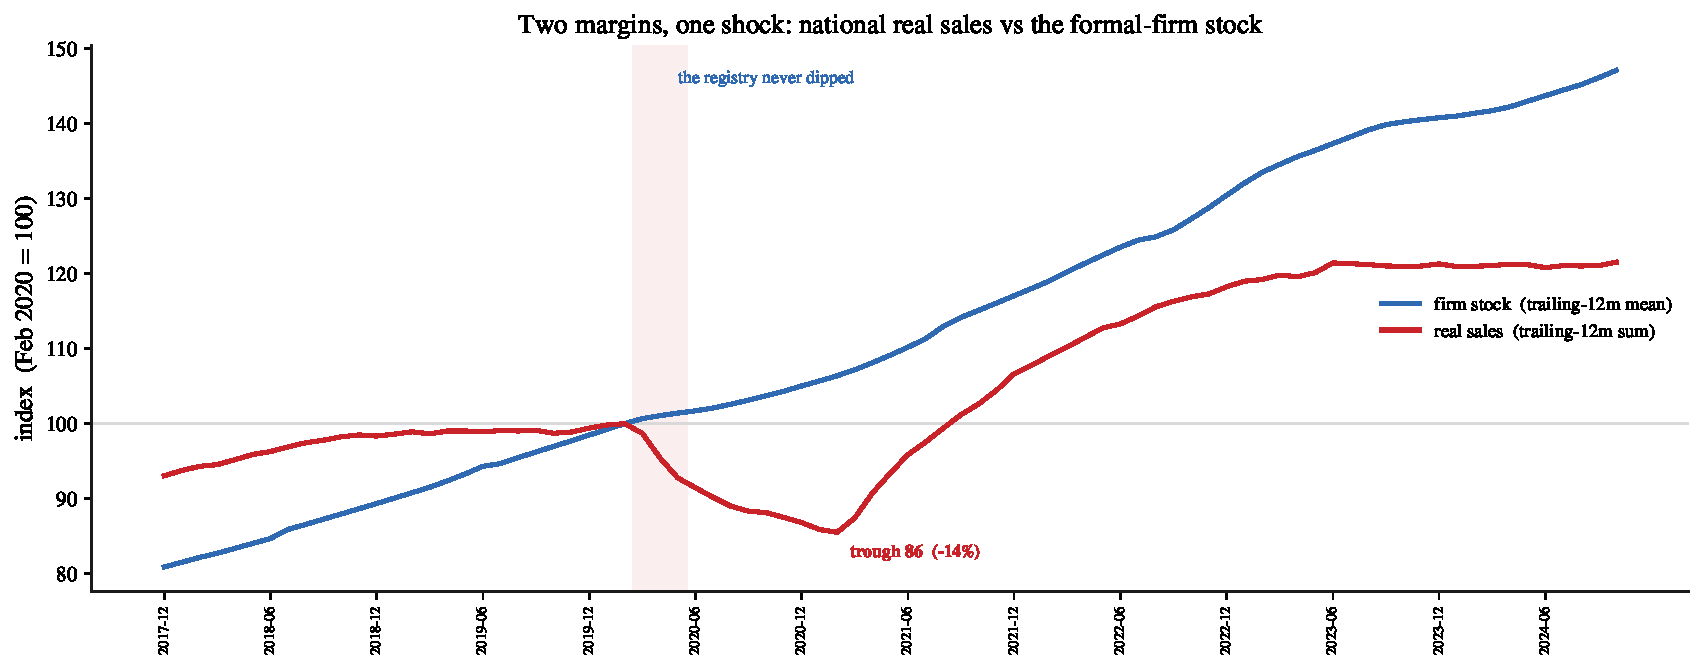
\includegraphics[width=\textwidth]{two_margins.pdf}
  \caption[Los dos márgenes durante la pandemia]{Los dos márgenes durante la pandemia: las ventas reales nacionales de los últimos doce meses (rojo) cayeron al 86~\% del nivel de febrero de 2020, mientras que el stock de empresas formales (azul) nunca descendió por debajo de su nivel previo al choque.}
  \label{fig:twomargins}
\end{figure}

En términos distributivos (Figura~\ref{fig:eras}), las tasas de crecimiento entre parroquias tienen colas marcadamente pesadas (los ajustes $t$ asimétricos superan a los gaussianos por márgenes de AIC de cientos, con índices de cola entre 1 y 2.4), mientras que el \textit{nivel} del logaritmo de las ventas es cercano a una distribución gaussiana: el sello clásico de Gibrat de tamaños lognormales y crecimiento desbocado. La pandemia desplazó la ubicación de las distribuciones de crecimiento e invirtió su asimetría (de $+1.1$, una cola derecha de parroquias en auge, a $-0.55$, una cola izquierda de parroquias en colapso, y de vuelta), pero dejó su dispersión esencialmente sin cambios: la desviación estándar entre parroquias se sitúa entre 0.74 y 0.83 en todos los años, incluido 2020. Un choque macroeconómico no dispersó los resultados; desplazó hacia abajo a todas las parroquias a la vez y generó una cola izquierda. El crecimiento de las ventas agrupado por era es de $+0.11$, $-0.23$ y $+0.22$ puntos logarítmicos por año; el crecimiento de las empresas es de $+0.14$, $+0.01$ y $+0.08$: se aplana, pero nunca se invierte.
\par

\begin{figure}[H]
  \setstretch{0.952}
  \centering
  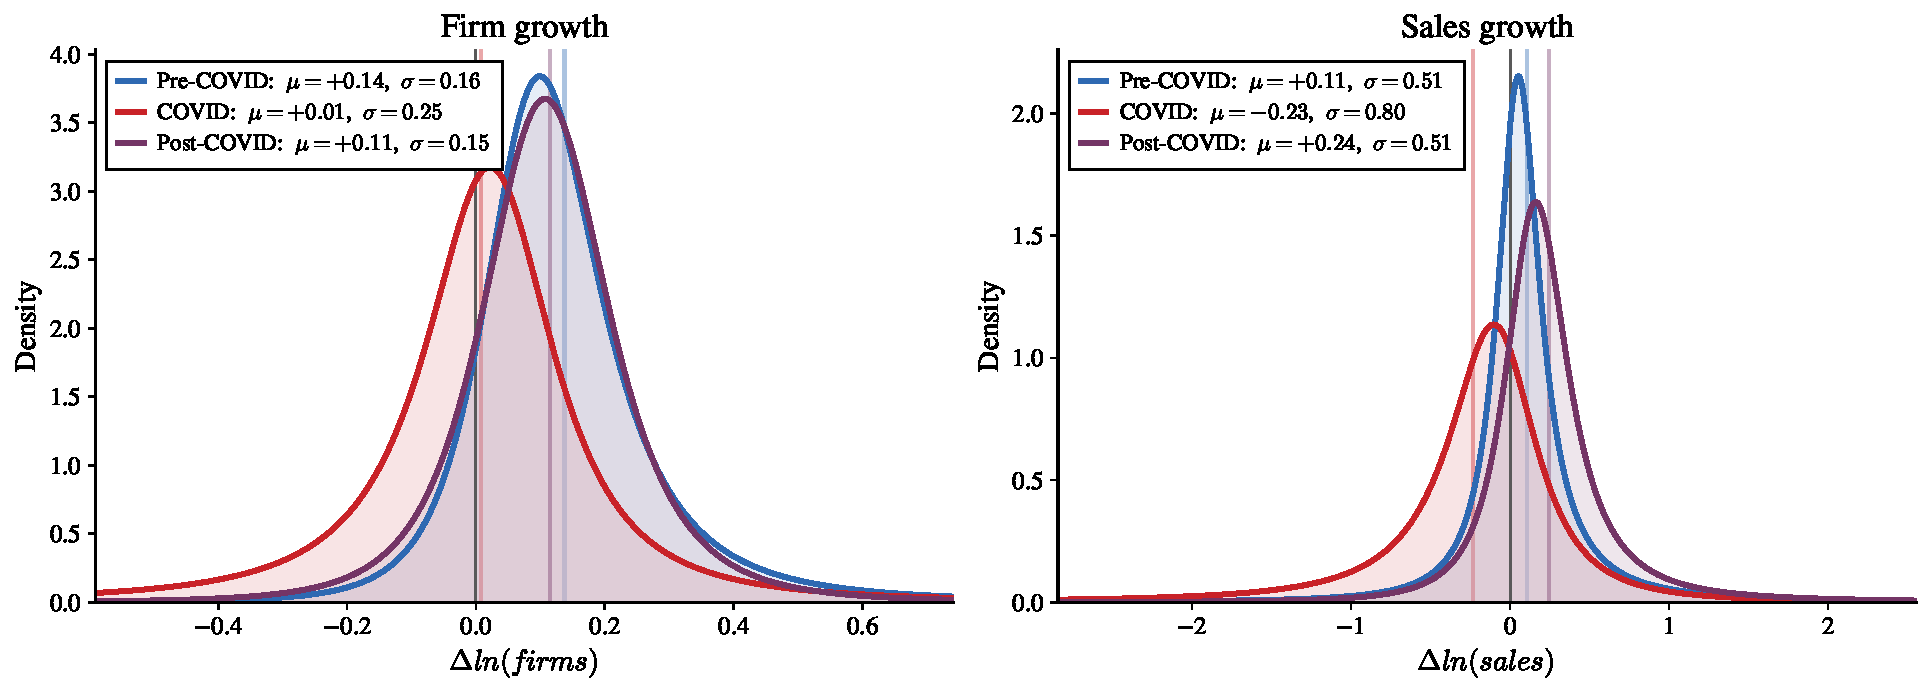
\includegraphics[width=\textwidth]{dist_overlay_eras.pdf}
  \caption[Distribuciones del crecimiento entre parroquias por era]{Distribuciones del crecimiento entre parroquias agrupadas en tres eras (antes, durante y después de la COVID): crecimiento del número de empresas (izquierda) y de las ventas reales (derecha). El choque desplazó la ubicación e invirtió la asimetría; no amplió la dispersión.}
  \label{fig:eras}
\end{figure}
\endgroup

% ----------- LA DESCOMPOSICIÓN PRINCIPAL Y SU ANATOMÍA DE ESCALA -----------
\clearpage
\blank
\tituloapa[La descomposición principal y su anatomía de escala]{LA DESCOMPOSICIÓN PRINCIPAL Y SU ANATOMÍA DE ESCALA}
\begingroup\dobleesp
\subtituloapa{Una reversión en seis años}
Durante toda la ventana, la vía de población se expresa, en puntos logarítmicos por año, como
\begin{equation*}
\underbrace{+0.0226}_{\text{cambio nacional}} =
\underbrace{-0.0270}_{\text{selección}} +
\underbrace{+0.0496}_{\text{transmisión}} .
\end{equation*}
El crecimiento real local por sí solo habría producido alrededor de un 5.1~\% anual; la reasignación del stock de empresas hacia lugares de bajas ventas devolvió más de la mitad. La Tabla~\ref{tab:annual} y la Figura~\ref{fig:byyear} muestran que la estructura es persistente y no un artefacto de los extremos de la ventana: la selección es negativa en cinco de seis pasos anuales y la transmisión es positiva en cinco de seis, con una única reversión simultánea en 2019$\to$2020, que se analiza en la sección sobre la inversión de 2019 a 2020 y cuyo signo depende de la definición del número de empresas (Tabla~\ref{tab:registro}). En la ventana previa al choque, 2017--2019, la dispersión fue lo suficientemente fuerte ($-0.0522$ por año) como para superar por completo a la transmisión, y el rasgo medio nacional de hecho \textit{cayó}.
\par

\begin{table}[H]
  \setstretch{0.952}
  \caption[Descomposición año por año, vía de población]{Descomposición año por año, vía de población (puntos logarítmicos por año). El año de la COVID invierte ambos términos a la vez.}
  \label{tab:annual}
  \begin{tabular}{|l|r|r|r|r|}
    \hline
    \textbf{Paso} & \textbf{Total} $\gamma^{p}$ & \textbf{Selección} $S^{p}$ & \textbf{Entre prov.} & \textbf{Transmisión} $T^{p}$ \\ \hline
    2017$\to$18 & $+0.0190$ & $-0.0451$ & $-0.0296$ & $+0.0641$ \\ \hline
    2018$\to$19 & $-0.0458$ & $-0.0597$ & $-0.0508$ & $+0.0139$ \\ \hline
    2019$\to$20 & $-0.1210$ & $\mathbf{+0.0342}$ & $+0.0149$ & $\mathbf{-0.1552}$ \\ \hline
    2020$\to$21 & $+0.1778$ & $-0.0346$ & $-0.0223$ & $+0.2124$ \\ \hline
    2021$\to$22 & $+0.0791$ & $-0.0338$ & $-0.0286$ & $+0.1129$ \\ \hline
    2022$\to$23 & $+0.0259$ & $-0.0183$ & $-0.0179$ & $+0.0442$ \\ \hline
  \end{tabular}
\end{table}

\begin{figure}[H]
  \setstretch{0.952}
  \centering
  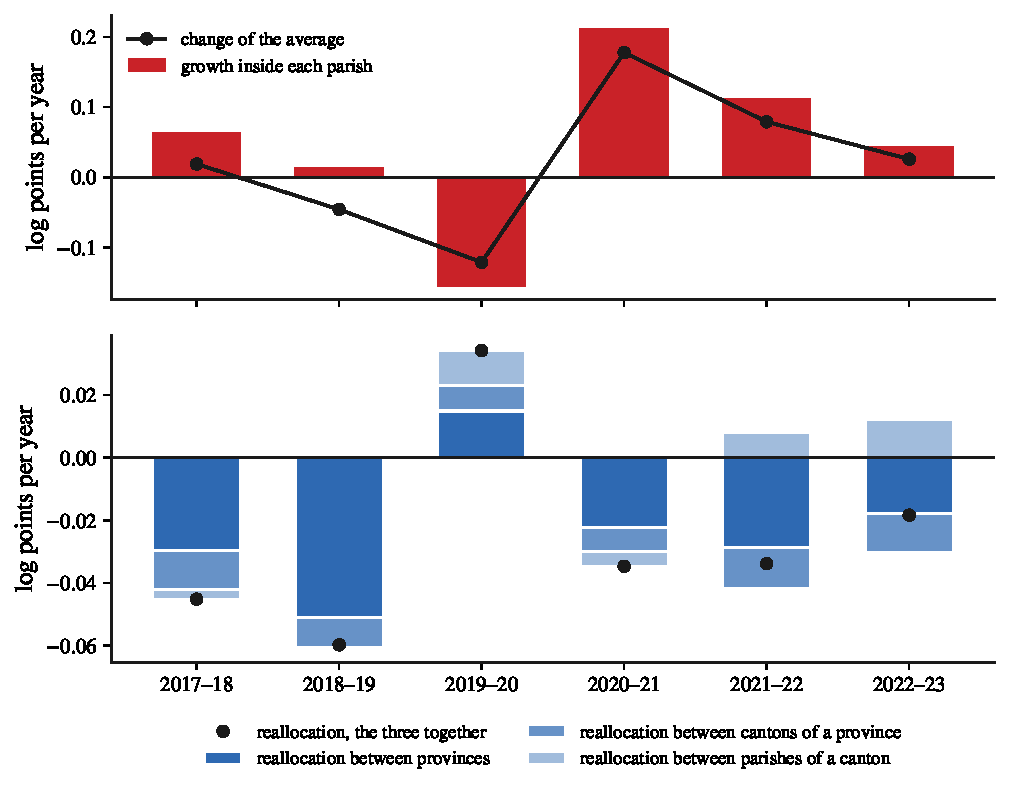
\includegraphics[width=0.85\textwidth]{change_by_year.pdf}
  \caption[La descomposición año por año, en sus partes]{La descomposición año por año, vía de población (puntos logarítmicos por año). Arriba: crecimiento dentro de cada parroquia (transmisión, barras) y cambio del promedio nacional (línea). Abajo: la selección dividida por escala (barras apiladas) y su total (punto). Los ejes verticales de los dos paneles son distintos, porque la transmisión es varias veces mayor que la selección. Solo en 2019$\to$2020 los tres componentes de la selección son positivos.}
  \label{fig:byyear}
\end{figure}

\subtituloapa{De qué está hecho el término de selección}
La partición del rasgo introducida en el Método responde a una pregunta que la cifra de $-0.0270$ deja abierta: si las empresas se forman en lugares \textit{pequeños} o en lugares donde las empresas \textit{venden poco}. Las dos cosas se confunden con facilidad, porque entre las 804 parroquias el logaritmo de las ventas totales y el del número de empresas tienen una correlación ponderada de $0.97$. La Tabla~\ref{tab:split} separa ambas partes (programa \texttt{trait\_split\_table.py} del repositorio); cada celda de la primera fila es la suma exacta de las dos siguientes. El 88~\% de la selección ($-0.0238$ de $-0.0270$) corresponde al tamaño: el número de empresas crece más rápido donde hay menos empresas, que es una desviación de la ley de Gibrat. Solo $-0.0032$ corresponde a las ventas por empresa, y ese componente no es estable: es negativo en cuatro de los seis pasos anuales y positivo en 2019$\to$2020 y en 2022$\to$2023. La lectura del resultado principal es, por tanto, que las empresas se dispersan hacia los lugares más pequeños, y no que lo hagan hacia lugares donde las empresas venden menos. La parte de tamaño se reparte entre provincias ($-0.0174$) y entre cantones ($-0.0096$); la de ventas por empresa solo existe entre provincias ($-0.0054$) y es prácticamente nula dentro de ellas.
\par

\begin{table}[H]
  \setstretch{0.952}
  \caption[Partición del rasgo de la vía de población, 2017--2023]{Partición del rasgo de la vía de población, 2017--2023 (por año). La primera fila es la descomposición principal; las otras dos la dividen de forma exacta según $\ln y_k = \ln n_k + \ln (y_k/n_k)$.}
  \label{tab:split}
  \small
  \begin{tabular}{|l|r|r|r|r|r|r|}
    \hline
    \textbf{Rasgo} & \textbf{Total} & \textbf{Selección} & \multicolumn{3}{c|}{\textbf{De la cual}} & \textbf{Transm.} \\ \cline{4-6}
     & $\gamma$ & $S$ & prov. & cantón & parroquia & $T$ \\ \hline
    Ventas totales, $\ln y_k$              & $+0.0226$ & $-0.0270$ & $-0.0227$ & $-0.0086$ & $+0.0043$ & $+0.0496$ \\ \hline
    Tamaño, $\ln n_k$                      & $+0.0707$ & $-0.0238$ & $-0.0174$ & $-0.0096$ & $+0.0031$ & $+0.0946$ \\ \hline
    Por empresa, $\ln (y_k/n_k)$           & $-0.0481$ & $-0.0032$ & $-0.0054$ & $+0.0010$ & $+0.0012$ & $-0.0449$ \\ \hline
  \end{tabular}
\end{table}

La tercera fila contiene además un resultado propio. El promedio, ponderado por empresas, del logaritmo de las ventas por empresa cayó $0.0481$ por año, y esa caída es casi toda transmisión ($-0.0449$) y muy poco selección ($-0.0032$): la reducción de las ventas por empresa descrita en la sección anterior ocurrió dentro de los lugares, incluidas las dos áreas metropolitanas, y no porque las empresas se desplazaran hacia lugares de menores ventas por empresa.
\par

\subtituloapa{Tres reponderaciones, un mismo patrón}
La Tabla~\ref{tab:threepaths} y la Figura~\ref{fig:monthly} someten la misma pregunta a las tres vías. Las afirmaciones cualitativas resisten cada reponderación: selección negativa y dominada por la escala entre provincias, transmisión positiva y mayor, y una única reversión en el paso 2019$\to$2020. Las magnitudes, en cambio, no son comparables entre vías, porque cada una pondera las parroquias de forma distinta: la vía de población las pondera por su participación de empresas, mientras que las de ingreso y de densidad lo hacen por esa participación multiplicada por el nivel, de modo que casi todo su peso recae en Quito y Guayaquil (véase el Método). Por eso la selección de las vías de ingreso y de densidad debe leerse como un contraste entre las dos áreas metropolitanas y el resto: su signo negativo indica que las ventas y el stock de empresas de Quito y Guayaquil crecieron más despacio que los de la parroquia promedio ponderada por empresas. Como la selección de la vía de densidad sería exactamente cero bajo la ley de Gibrat, su valor persistentemente negativo (en cinco de seis años y a través de todas las lentes trimestrales) constituye un rechazo del crecimiento proporcional en favor de un crecimiento inclinado hacia la periferia; la parte de tamaño de la Tabla~\ref{tab:split} es la misma prueba en logaritmos, no está dominada por dos parroquias, es exacta en todas las escalas y llega a la misma conclusión.
\par

\begin{table}[H]
  \setstretch{0.952}
  \caption[Las tres vías, 2017--2023]{Las tres vías, 2017--2023 (por año). La selección se divide por escala según la Ecuación~\eqref{eq:multiscale}.}
  \label{tab:threepaths}
  \small
  \begin{tabular}{|l|r|r|r|r|r|r|}
    \hline
    \textbf{Vía} & \textbf{Total} & \textbf{Selección} & \multicolumn{3}{c|}{\textbf{De la cual}} & \textbf{Transm.} \\ \cline{4-6}
     & $\gamma$ & $S$ & prov. & cantón & parroquia & $T$ \\ \hline
    pob & $+0.0226$ & $-0.0270$ & $-0.0227$ & $-0.0086$ & $+0.0043$ & $+0.0496$ \\ \hline
    ing & $+0.0315$ & $-0.0148$ & $-0.0093$ & $-0.0037$ & $-0.0018$ & $+0.0463$ \\ \hline
    den & $+0.0826$ & $-0.0074$ & $-0.0073$ & $-0.0022$ & $+0.0021$ & $+0.0900$ \\ \hline
  \end{tabular}
\end{table}

\begin{figure}[H]
  \setstretch{0.952}
  \centering
  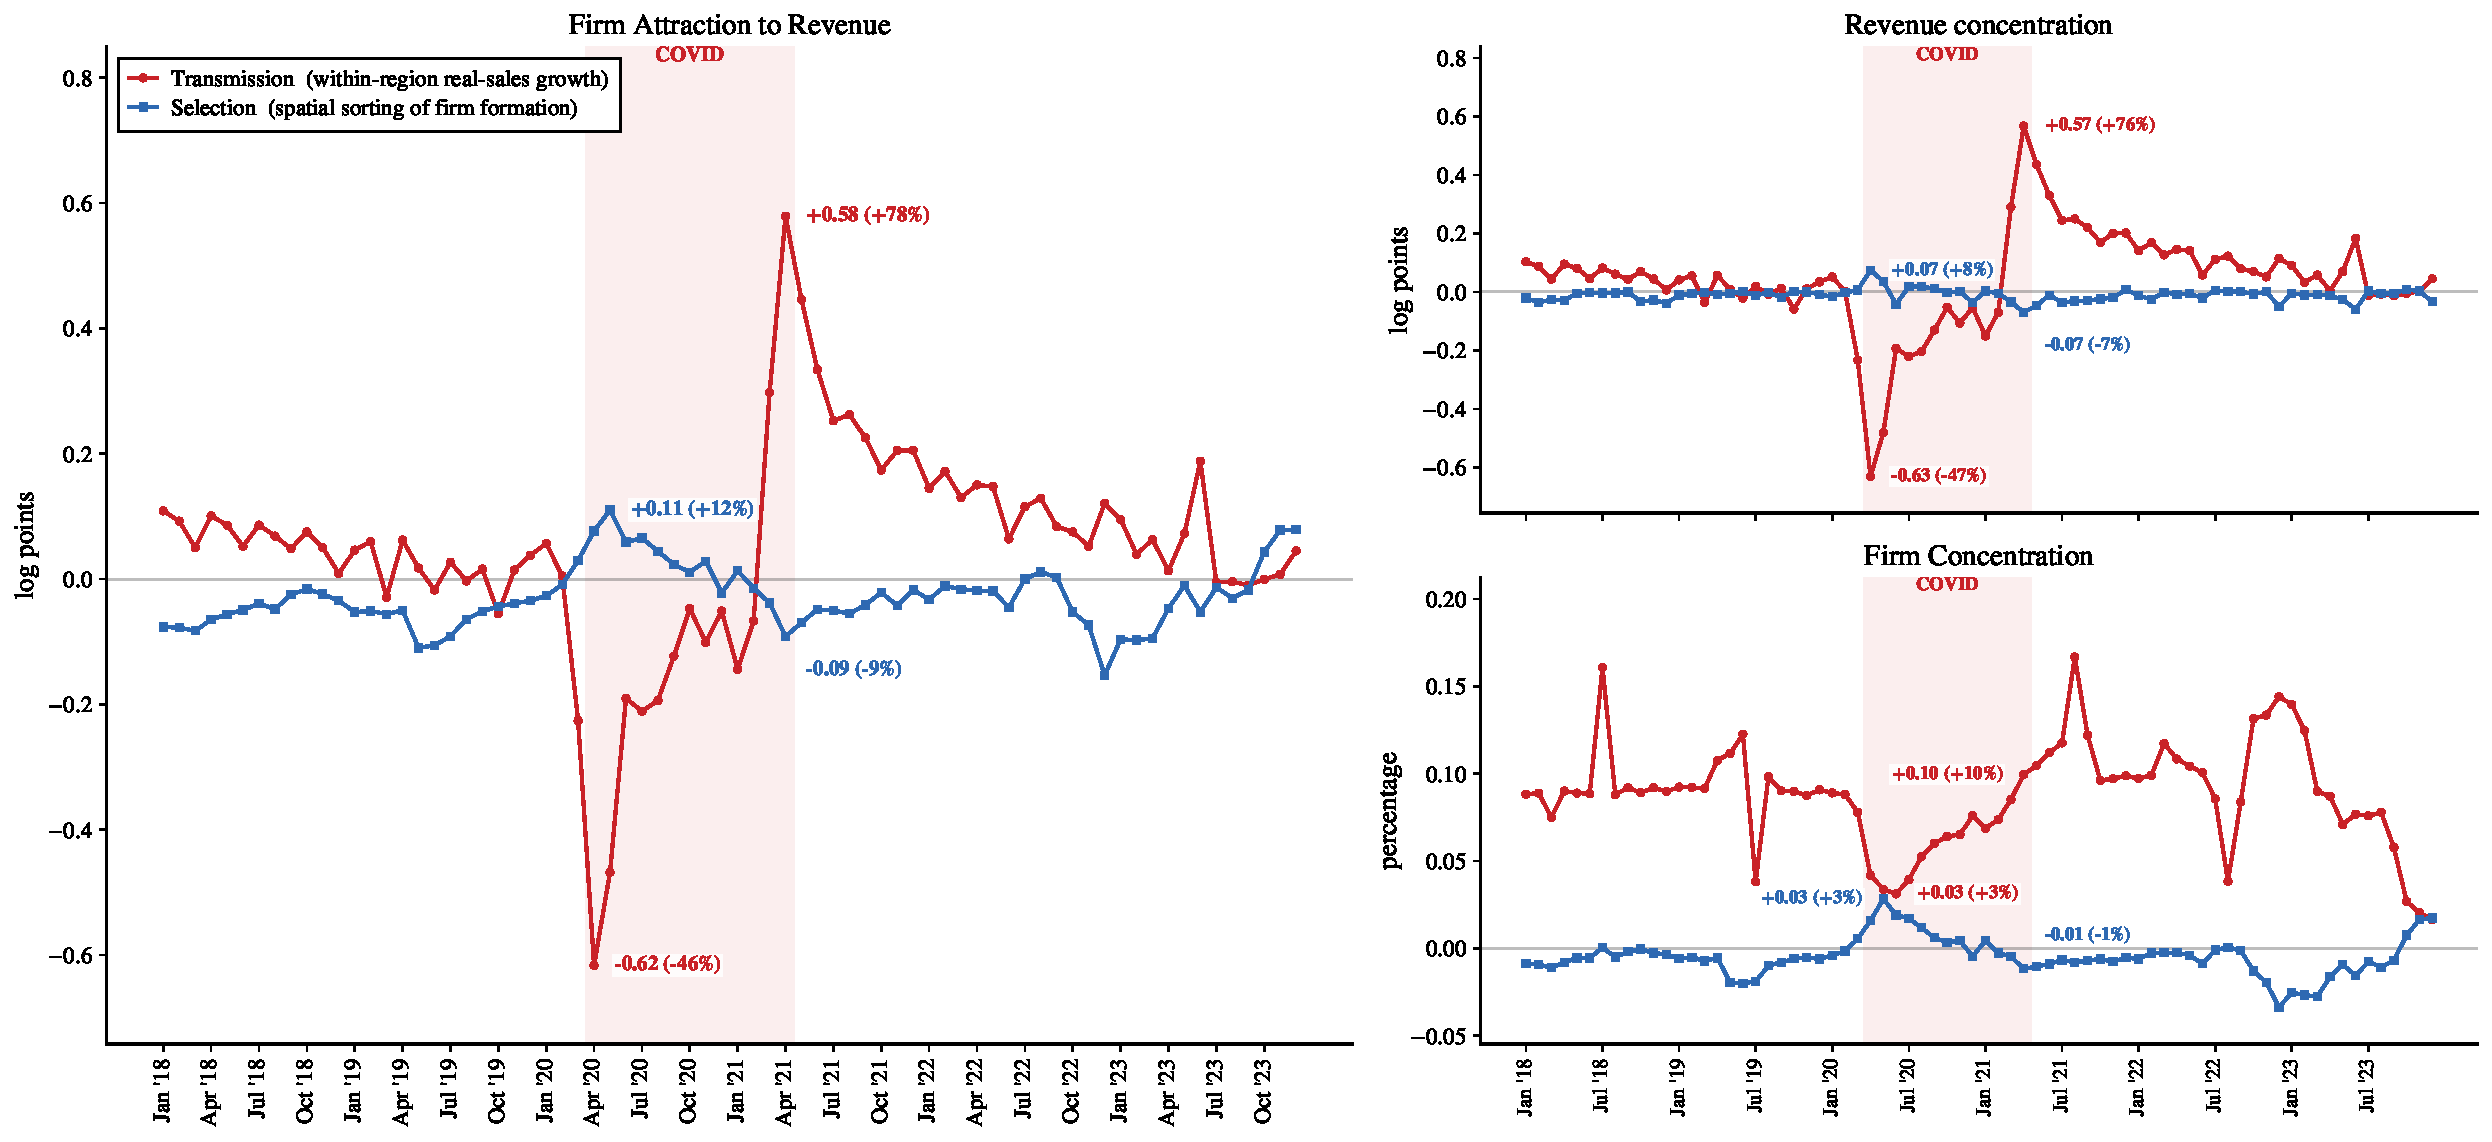
\includegraphics[width=\textwidth]{monthly_timeseries_all_paths.pdf}
  \caption[Selección y transmisión mensuales en las tres vías]{Selección y transmisión en las tres vías a lo largo de 72 ventanas móviles de doce meses. Las tres series de selección son negativas en tiempos normales; la transmisión colapsa a $-0.62$ (anualizada; $-46$~\% interanual) en la ventana que termina en abril de 2020, mientras la selección se vuelve positiva.}
  \label{fig:monthly}
\end{figure}

\subtituloapa{La anatomía de escala}
La división multiescala \eqref{eq:multiscale} localiza la dispersión (Tabla~\ref{tab:threepaths}; Figura~\ref{fig:waterfall} para la vía de población), y los tres componentes merecen describirse por separado, porque ninguno es cero. El mayor es el término \textit{entre provincias}: $-0.0227$ de los $-0.0270$ de la selección de la vía de población, el 84~\%, negativo en cinco de los seis pasos anuales. El segundo, la selección \textit{entre cantones dentro de cada provincia}, vale $-0.0086$ por año, un tercio de la selección total (las participaciones suman más de 100~\% porque el tercer componente tiene signo contrario); es menor que el término entre provincias, pero no es despreciable: tiene el mismo signo en los cinco pasos anuales normales y en la ventana completa, y en 2022$\to$2023 alcanza $-0.0125$, cerca de tres cuartos del término entre provincias de ese año. Dentro de las provincias, los cantones de menores ventas también ganan empresas más rápido que los de mayores ventas. El tercero, la selección \textit{entre parroquias dentro de cada cantón}, es el más pequeño ($+0.0043$ en la ventana completa, un $-16$~\% de la selección) y el único de signo cambiante: $-0.0031$ y $+0.0008$ en los dos primeros pasos, $+0.0112$ en 2019$\to$2020, $-0.0048$ en 2020$\to$2021 y de nuevo positivo en los dos últimos ($+0.0080$ y $+0.0121$). Es decir, dentro de los cantones las parroquias de mayores ventas (en general, las cabeceras) han sumado empresas algo más rápido que sus periferias desde 2021, un cambio de régimen que la sección sobre la inversión retoma. Es también la única escala en la que las tres vías discrepan en el signo (Tabla~\ref{tab:threepaths}), por lo que su lectura es la más provisional de las tres. Expresadas en porcentaje del crecimiento nacional, las celdas de la vía de población son $+18.8$, $-37.9$, $-100.4$ y $+219.5$, que suman exactamente 100: el crecimiento dentro de las parroquias aportó 2.2 veces el cambio nacional efectivo, la selección entre provincias por sí sola restó una cantidad igual a todo el cambio nacional y la selección entre cantones restó algo más de un tercio.
\par

\begin{figure}[H]
  \setstretch{0.952}
  \centering
  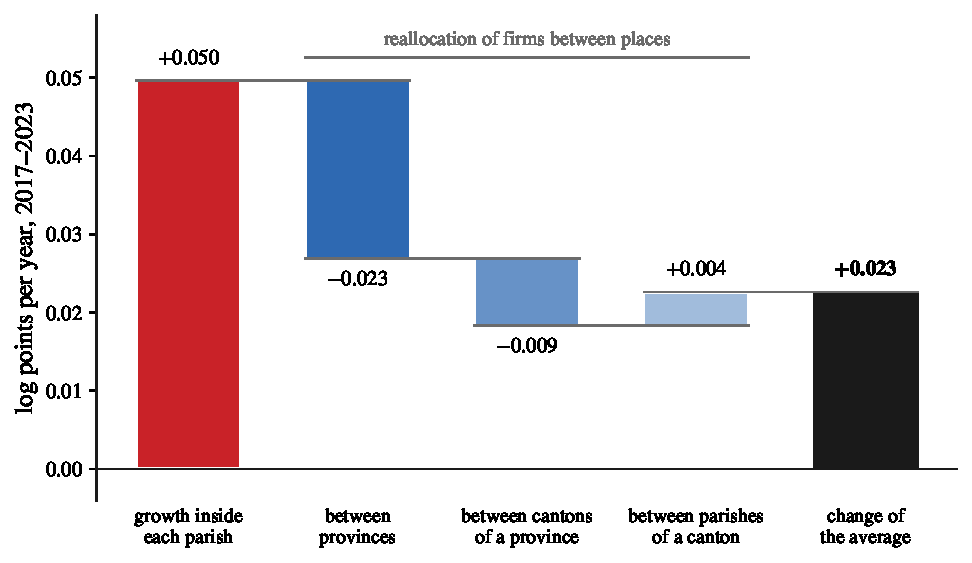
\includegraphics[width=0.8\textwidth]{change_waterfall.pdf}
  \caption[De dónde proviene el cambio del promedio nacional]{De dónde proviene el cambio del promedio nacional, vía de población, 2017--2023 (puntos logarítmicos por año). Cada barra parte de donde terminó la anterior: al crecimiento dentro de cada parroquia (transmisión, $+0.050$) se suman los tres componentes de la selección, entre provincias ($-0.023$), entre cantones de una misma provincia ($-0.009$) y entre parroquias de un mismo cantón ($+0.004$); la última barra es el total ($+0.023$).}
  \label{fig:waterfall}
\end{figure}

La Figura~\ref{fig:scales} muestra el mismo hecho en los datos originales: la nube crecimiento--tamaño se inclina en los tres niveles, pero con pendientes muy distintas. En 2018$\to$2019 la correlación ponderada entre crecimiento y tamaño es de $-0.10$ entre parroquias, $-0.21$ entre cantones y $-0.79$ entre provincias; en la ventana completa 2017$\to$2023 las pendientes ponderadas son $-0.0018$, $-0.0034$ y $-0.0046$. La dinámica empresarial del Ecuador es, por tanto, \textit{casi} libre de escala a nivel local, con una inclinación débil pero del mismo signo entre cantones, y claramente convergente a nivel regional. Una regresión de crecimiento en una sola escala, agrupada entre parroquias, reportaría una desviación pequeña de la ley de Gibrat y subestimaría el efecto; y una reforma evaluada sobre resultados parroquiales o cantonales mediría solo una fracción del efecto espacial, porque la mayor parte de la señal se encuentra uno o dos niveles de agregación más arriba. La velocidad del proceso puede leerse directamente en las participaciones: entre 2017 y 2023, la parte del stock de empresas ubicada en las cabeceras de Quito y Guayaquil pasó de 56.5~\% a 52.9~\%, es decir, 3.5 puntos porcentuales en seis años. La desconcentración espacial es real, y es lenta.
\par

\begin{figure}[H]
  \setstretch{0.952}
  \centering
  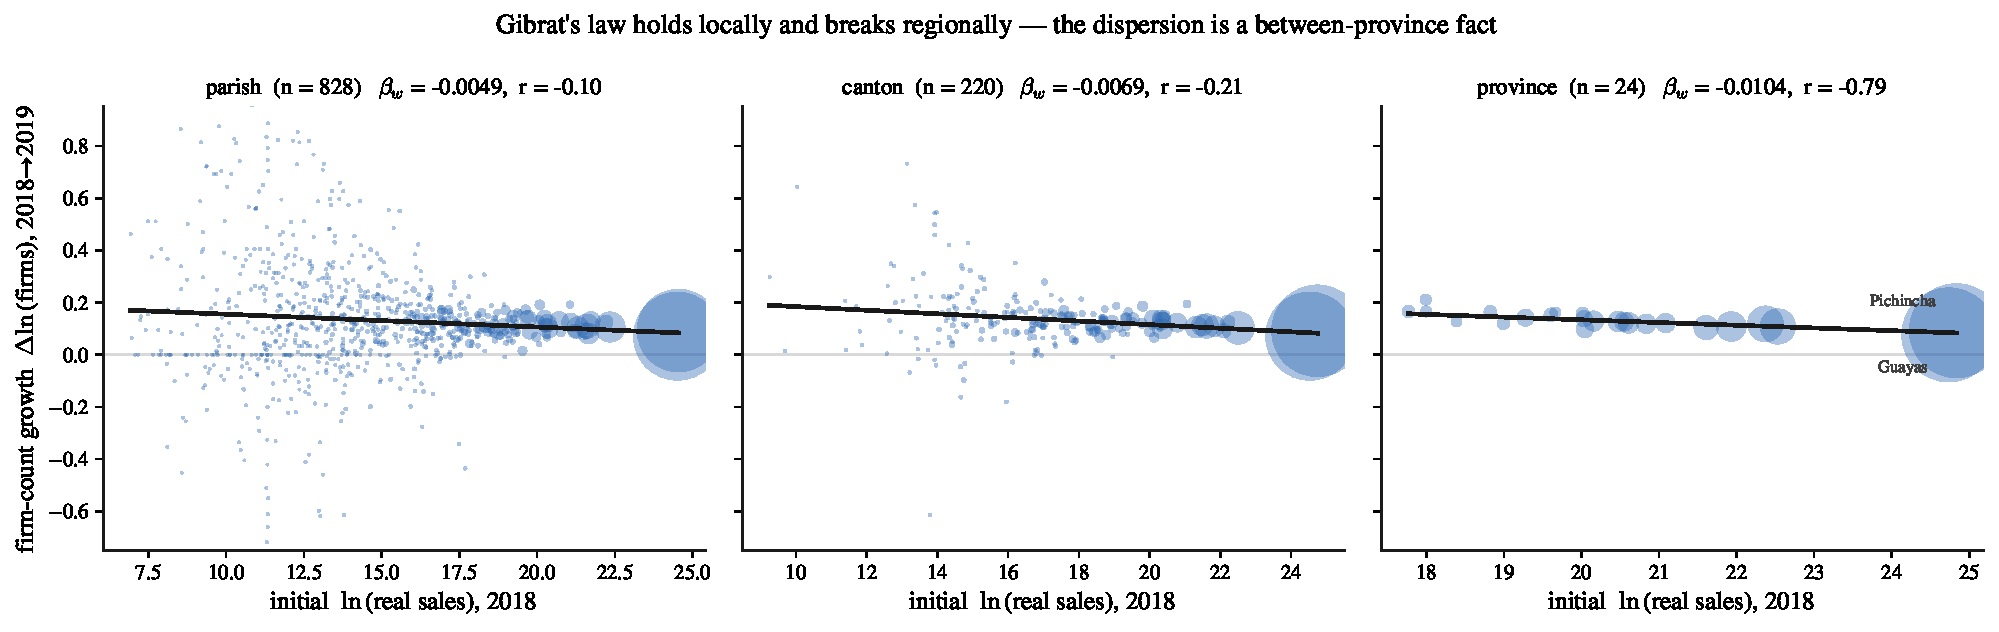
\includegraphics[width=\textwidth]{scale_scatters.pdf}
  \caption[Crecimiento frente a tamaño en los tres niveles anidados]{Crecimiento del número de empresas frente al logaritmo inicial de las ventas reales en los tres niveles anidados (2018$\to$2019). La nube se inclina poco en las escalas parroquial y cantonal y de forma decisiva entre provincias: la ley de Gibrat se cumple aproximadamente a escala local y se rompe a escala regional.}
  \label{fig:scales}
\end{figure}

\subtituloapa{Quién protagoniza el efecto}
Descomponer el término entre provincias mediante \eqref{eq:contribution} revela un movimiento de pinza. Desde arriba: Guayas concentra el 34~\% de las empresas, se ubica $+1.76$ puntos logarítmicos por encima del rasgo medio y su stock de empresas creció un 5.4~\% más lento que el promedio nacional, de modo que una sola provincia aporta una cuarta parte de todo el término entre provincias. Desde abajo: provincias amazónicas como Morona Santiago (0.4~\% de las empresas, 6.9 puntos logarítmicos por debajo de la media, crecimiento empresarial un 34~\% superior al promedio) empujan la misma covarianza hacia valores negativos. La influencia está concentrada (la mayor contribución parroquial individual, la del centro de Guayaquil, equivale al 19~\% de la suma de las contribuciones absolutas), pero se concentra en los propios centros económicos, cuyo peso proviene de su \textit{participación} de empresas y no de tasas de crecimiento extremas; la parroquia más explosiva del país (una parroquia de Morona Santiago que pasó de 8 a 101 empresas) no aporta casi nada, porque su peso es $7 \times 10^{-5}$. La sección de Robustez formaliza esta distinción.
\par
\endgroup

% ------------------------ LA INVERSIÓN PANDÉMICA ------------------------
\clearpage
\blank
\tituloapa[La inversión de 2019 a 2020]{LA INVERSIÓN DE 2019 A 2020}
\begingroup\dobleesp
\vspace{6pt}
El paso 2019$\to$2020 coincide con la pandemia de COVID-19 y con el confinamiento de marzo a junio de 2020. Esta sección describe en qué se distinguió ese paso de los demás y quién protagonizó la diferencia; como se advirtió en el Método, no atribuye la diferencia a la pandemia, porque el diseño no dispone de un contrafactual.
\par
\subtituloapa{La inversión, dibujada y no inferida}
En 2019$\to$2020 la selección se invierte a $+0.0342$, mientras la transmisión colapsa a $-0.1552$ (Tabla~\ref{tab:annual}), y la inversión aparece en las tres escalas a la vez: $+0.015$ entre provincias, $+0.008$ entre cantones dentro de las provincias y $+0.011$ entre parroquias dentro de los cantones. Aparece también en las dos partes del rasgo: $+0.0233$ en la de tamaño y $+0.0109$ en la de ventas por empresa. Como la selección es exactamente la inclinación de la nube aptitud--rasgo, la Figura~\ref{fig:tilt} muestra la reversión en los datos originales y no en un coeficiente: la pendiente pasa por $-0.045$ y $-0.060$, luego $+0.034$ en el panel de la pandemia, y después $-0.035$, $-0.034$ y $-0.018$. El mecanismo es visible en ambos cuadrantes de la covarianza: el crecimiento nacional del stock se desaceleró (6.7~\%, frente a entre 8.0 y 11.5~\% en los demás pasos), el enjambre de parroquias pequeñas y de bajas ventas cayó por debajo de la nueva vara y las áreas metropolitanas se mantuvieron justo por encima, una reconcentración breve que deshizo en un paso el equivalente a un año de la lenta dispersión. Un año después, el sistema se recuperó con la mayor transmisión de la muestra ($+0.2124$).
\par

Este resultado se refiere a la población del estudio, las sociedades en actividades con ventas declaradas, y debe leerse con ella. El mismo cálculo sobre el catastro completo de sociedades activas, incluidas las de celdas sin ninguna declaración, que es otro objeto de estudio, da una selección de $-0.0021$ en 2019$\to$2020 (frente a $+0.0342$) y de $-0.0003$ en 2020$\to$2021 (frente a $-0.0346$; Tabla~\ref{tab:registro}). La diferencia entre los dos objetos puede verse directamente en los conteos. Entre 2019 y 2020 el stock de todas las sociedades activas creció casi lo mismo en todos los tamaños de parroquia: 8.1~\% en las que tenían menos de diez sociedades, 7.4~\% en las de diez a cincuenta, 6.7~\% en las de cincuenta a quinientas y 7.4~\% en las de más de quinientas. El stock en celdas con ventas declaradas, en cambio, creció 0.1, 1.1, 5.1 y 7.4~\%, porque en las parroquias pequeñas aumentó la proporción de sociedades activas situadas en celdas donde ninguna declaró ventas: del 54 al 60~\% en las de menos de diez sociedades y del 26 al 30~\% en las de diez a cincuenta (en el país, del 3.1~\% en 2019 a un máximo de 4.9~\% en abril de 2020). La inversión no describe, por tanto, sociedades que cierran en la periferia o que se trasladan a los centros: el stock de sociedades activas siguió creciendo al mismo ritmo en todas partes, y lo que se concentró fue la actividad con ventas declaradas, porque en los lugares pequeños más actividades dejaron de declarar. En ninguno de los dos objetos continuó la dispersión entre 2019 y 2021: se invirtió en la población con actividad declarada y se detuvo en el catastro. El signo positivo de la selección de ese paso es, en consecuencia, un resultado sobre la actividad con ventas declaradas y no sobre el catastro, y la anatomía que sigue (quién protagoniza la inversión) describe a esa población.
\par

\begin{figure}[H]
  \setstretch{0.952}
  \centering
  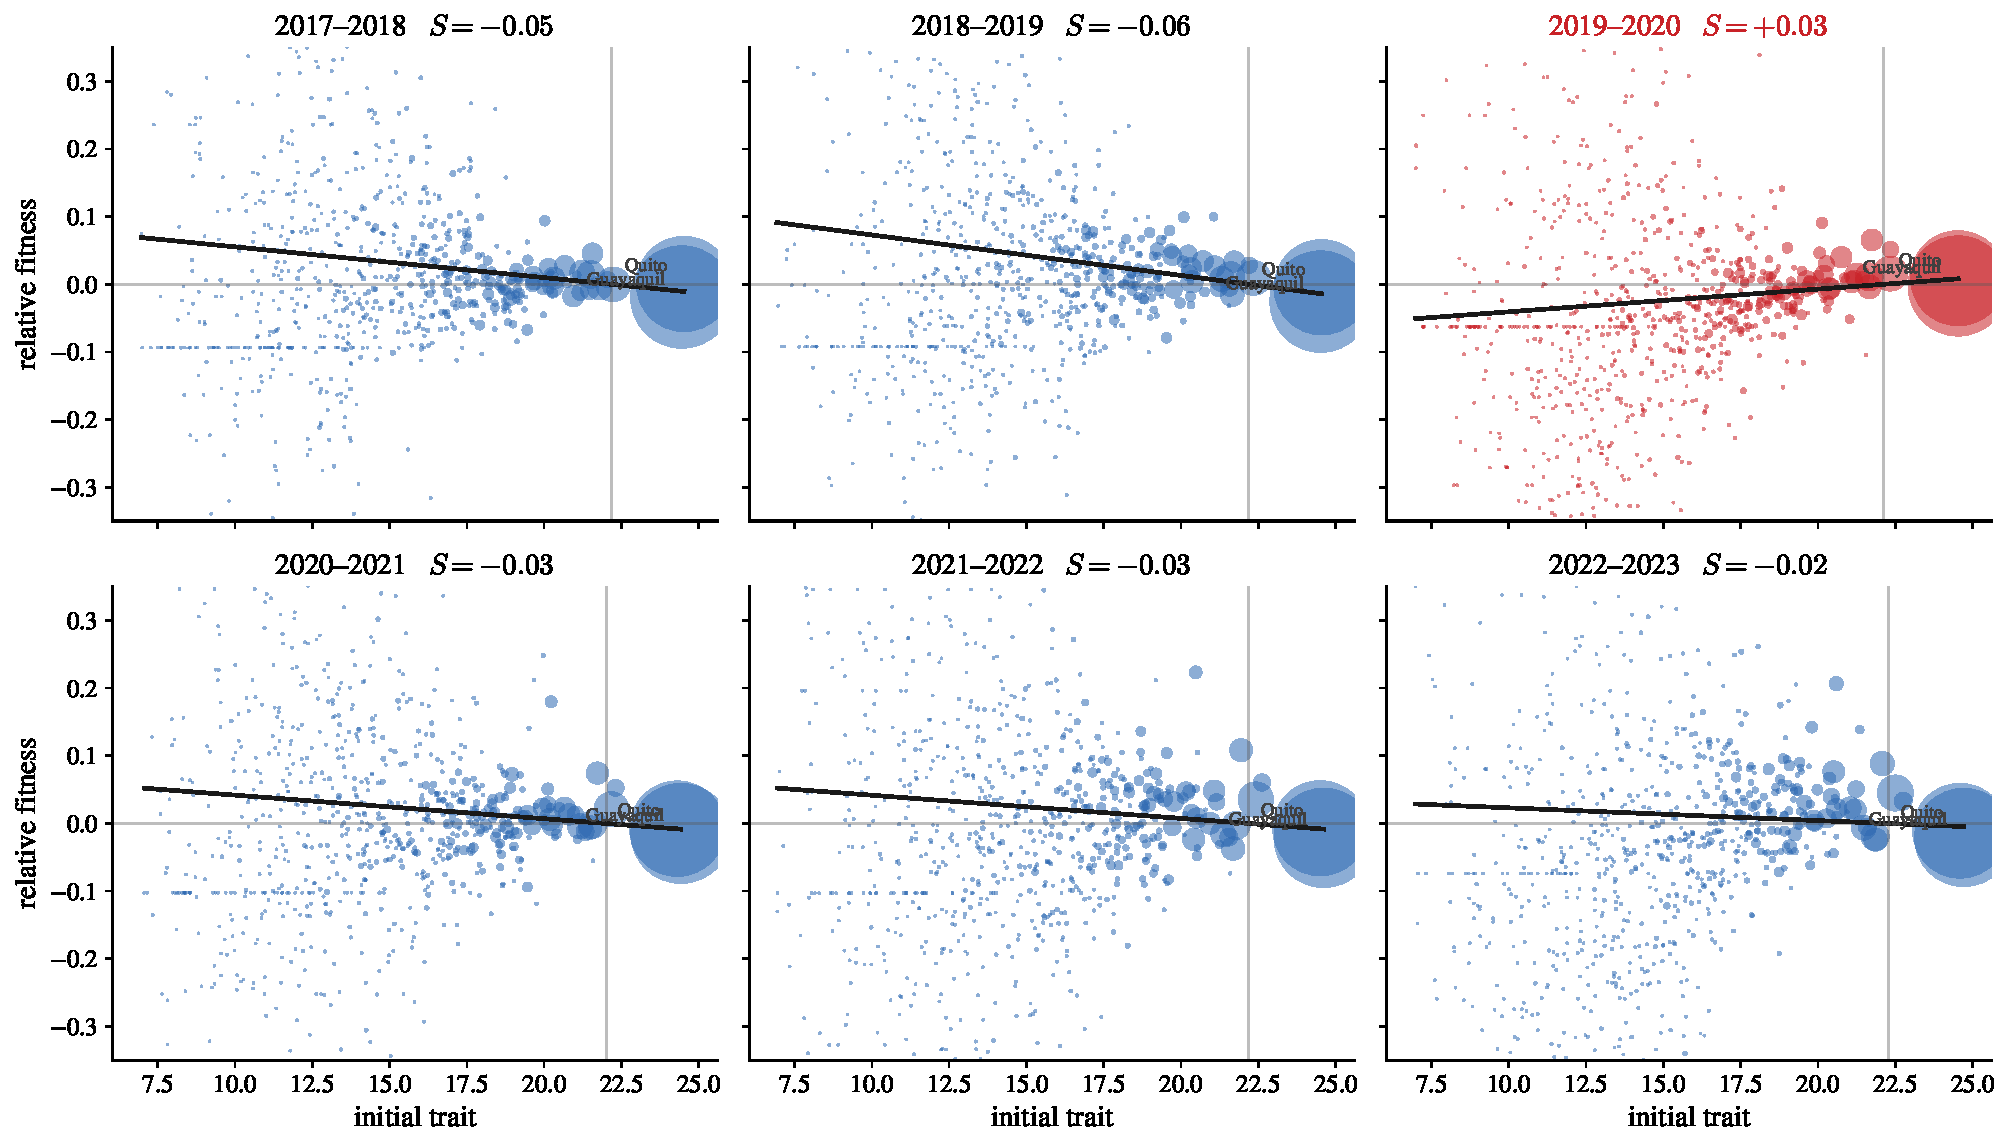
\includegraphics[width=\textwidth]{selection_flip_scatter.pdf}
  \caption[La selección como inclinación, por paso anual]{La selección como inclinación, un panel por paso anual. Cada punto es una parroquia en (logaritmo inicial de las ventas reales, aptitud relativa del número de empresas), con área proporcional a su participación de empresas; la línea es la regresión ponderada por participación de empresas, cuya pendiente multiplicada por la varianza del rasgo \textit{es} el término de selección. Todos los años normales se inclinan hacia abajo; 2019$\to$2020 se inclina hacia arriba.}
  \label{fig:tilt}
\end{figure}

Dos descripciones alternativas no se sostienen en los datos. La proximidad no organiza la inversión: un gradiente de distancia a los centros entre parroquias es estadísticamente nulo en general y sobrevive solo como una leve inclinación dentro de las provincias que explica alrededor del 1~\% de la varianza; la variable asociada al resultado de una parroquia fue su propio tamaño y no su distancia a un área metropolitana. Tampoco la inversión es un artefacto de valores atípicos: la sostienen cientos de parroquias ordinarias, y las distribuciones no ponderadas entre parroquias no cambian cuando se excluyen Quito y Guayaquil.
\par

\subtituloapa{Qué hizo diferente a Quito}
La Figura~\ref{fig:carriers} identifica a los protagonistas, y una ciudad encabeza ambas listas. Quito es el mayor contribuyente positivo individual a la selección ($+0.56$~\% anual, el 16.4~\% de todo el término) \textit{y} el mayor lastre individual de la transmisión ($-5.95$~\% anual, el 38.3~\% de ese término, con Guayaquil en segundo lugar con el 20.9~\%). Durante el paso 2019$\to$2020, Quito siguió sumando empresas más rápido que cualquier otro lugar del país ($+7.65$ puntos logarítmicos, frente a $+6.43$ de Guayaquil y un $+6.7$ nacional ponderado por empresas), mientras sus propias ventas cayeron más que las de cualquier otra área metropolitana ($-0.22$ frente a $-0.11$ de Guayaquil, en logaritmos). Dentro de una misma ciudad, los márgenes extensivo e intensivo se separaron.
\par

\begin{figure}[H]
  \setstretch{0.952}
  \centering
  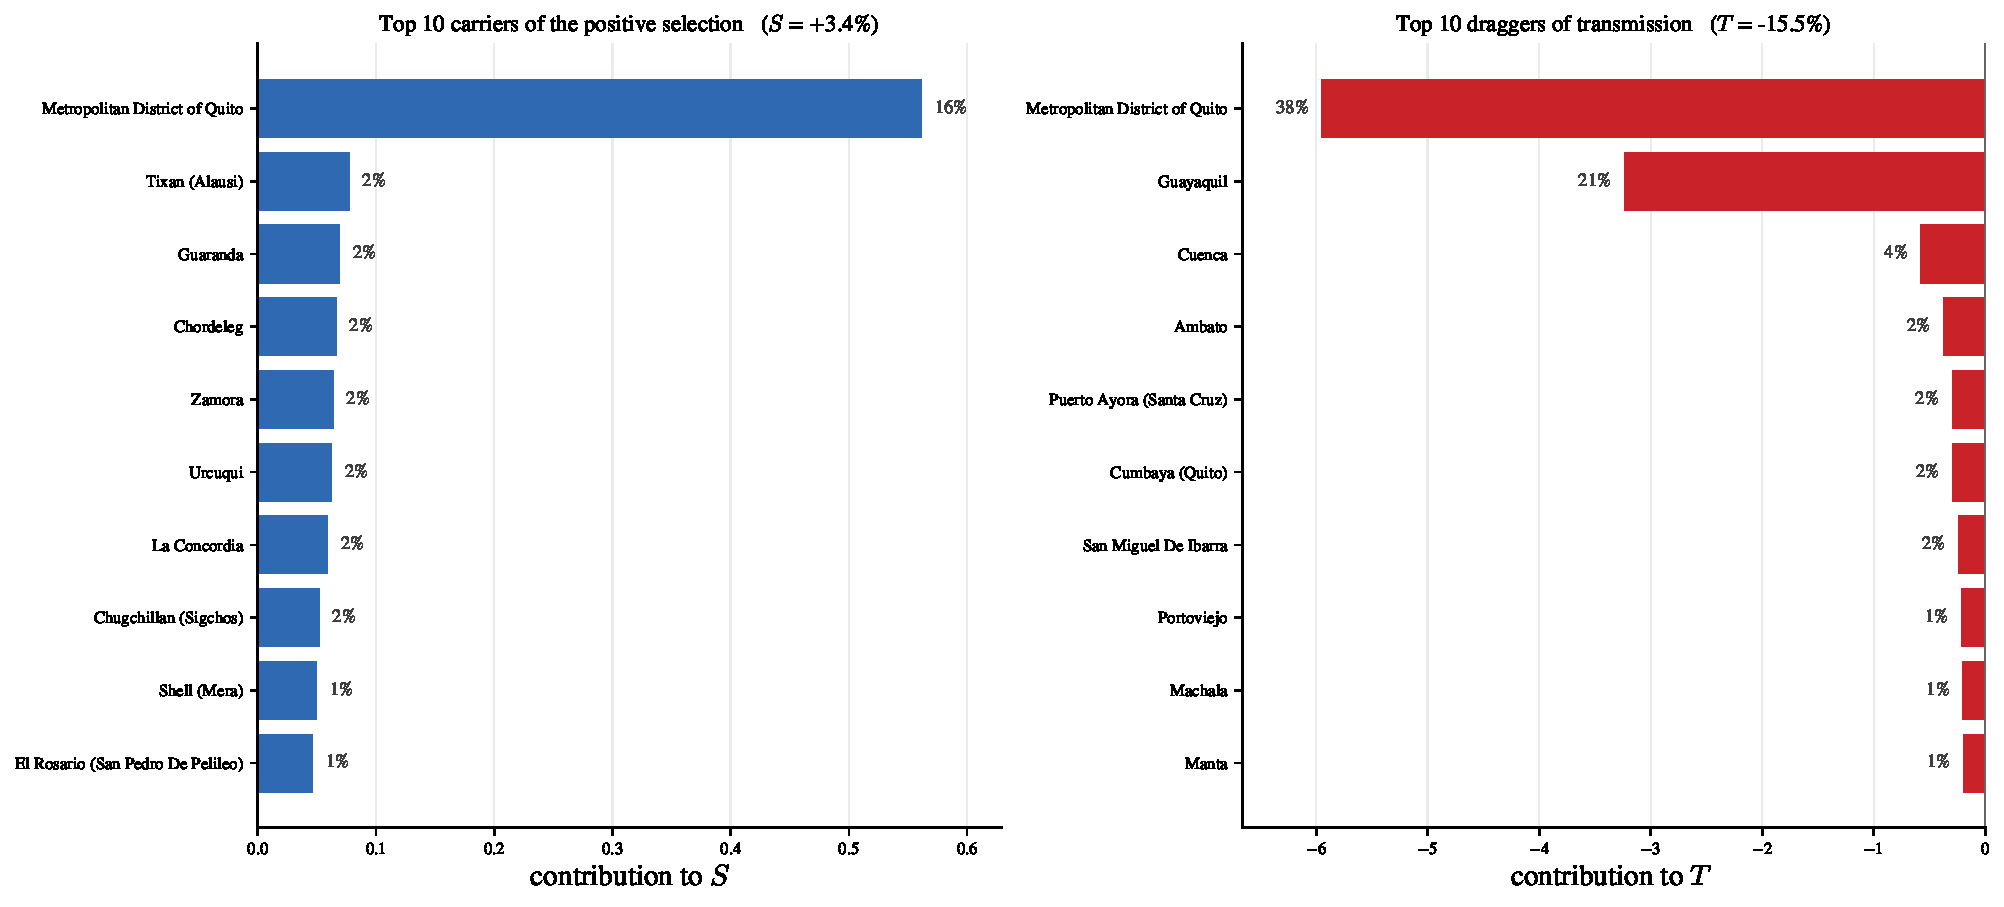
\includegraphics[width=\textwidth]{covid_carriers_bars.pdf}
  \caption[Mayores contribuciones parroquiales en 2019$\to$2020]{Mayores contribuciones parroquiales a los términos de selección (arriba) y transmisión (abajo) de 2019$\to$2020. Quito es a la vez el mayor contribuyente positivo a la selección y el mayor lastre de la transmisión.}
  \label{fig:carriers}
\end{figure}

La brecha de 1.22 puntos tiene una dirección en el espacio de actividades (Figura~\ref{fig:sectors}): solo los servicios profesionales y científicos aportan $+0.45$, seguidos por las finanzas, las actividades inmobiliarias, la información y los servicios administrativos y de apoyo, todos ellos servicios susceptibles de teletrabajo. El control es el comercio, el mayor contribuyente en ambas ciudades, que creció a un ritmo idéntico ($+1.7$ frente a $+1.8$); por lo tanto, la ventaja de la capital se asocia con su composición sectorial y no con su tamaño ni con un rasgo urbano general. Una hipótesis coherente con este patrón es que el ecosistema de servicios profesionales de Quito ofreció un margen de registro que una economía portuaria y de transporte no ofrecía, en parte como emprendimiento por necesidad (actividades que un trabajador desplazado puede registrar y operar desde casa); los datos describen el patrón, pero no permiten probar esa hipótesis ni descartar otras.
\par

\begin{figure}[H]
  \setstretch{0.952}
  \centering
  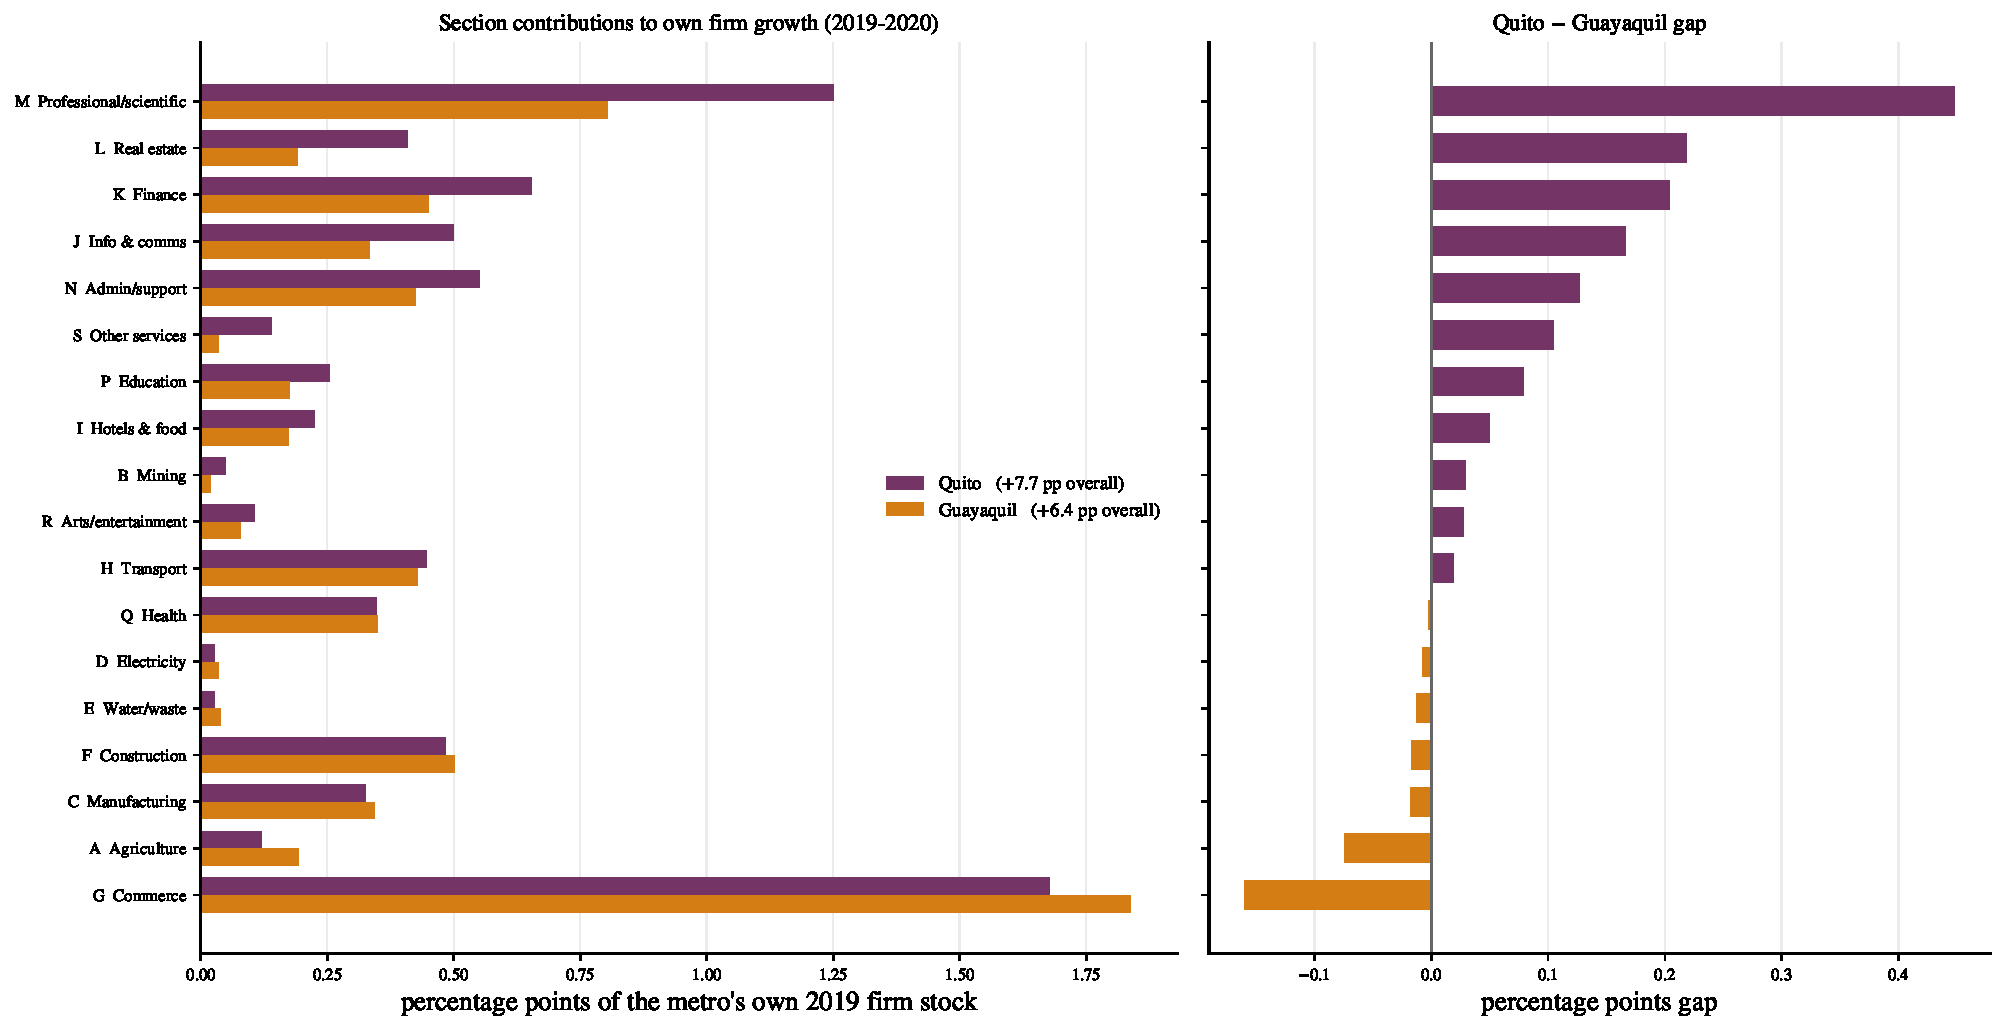
\includegraphics[width=\textwidth]{metro_sector_contributions.pdf}
  \caption[Contribuciones sectoriales, Quito frente a Guayaquil]{Contribuciones sectoriales al crecimiento del stock de empresas durante el paso de la COVID, Quito frente a Guayaquil, con la brecha por sector. La ventaja de la capital se concentra en servicios susceptibles de teletrabajo; el comercio, el mayor contribuyente en ambas ciudades, es idéntico.}
  \label{fig:sectors}
\end{figure}

La misma geografía del número de empresas presenta un segundo cambio de régimen, más discreto: en las ventanas que terminan después de octubre de 2022, el componente de la selección de la vía de población correspondiente a las parroquias dentro de los cantones se desacopla de la escala superior y se vuelve positivo, y en la vía de densidad la correlación entre la selección a nivel cantonal y a nivel parroquial se invierte de $+0.77$ a $-0.40$, mientras que la vía de ingreso no muestra ninguna ruptura ($+0.57$ a $+0.58$). Las dos vías que se rompen están determinadas por el número de empresas, y la que no se rompe, por las ventas: la ruptura se refiere a dónde se ubican las empresas y no a dónde están las ventas (las parroquias centrales de las capitales provinciales medianas empezaron a sumar más empresas que sus propias periferias), y una sola descomposición no habría podido indicar cuál.
\par
\endgroup

% ------------------ CUANDO EL PROMEDIO NO ES UNA DESCRIPCIÓN ------------------
\clearpage
\blank
\tituloapa[Cuando el promedio no es una descripción]{CUANDO EL PROMEDIO NO ES UNA DESCRIPCIÓN}
\begingroup\dobleesp
\subtituloapa{Cuatro regímenes dentro de un agregado plano}
La selección y la transmisión llevan cada una un signo por unidad, de modo que cada parroquia cae en uno de cuatro regímenes: \textit{expansión} (gana empresas y aumenta sus ventas), \textit{consolidación} (empresas estables, ventas crecientes), \textit{dilución} (más empresas que se reparten menos dólares) y \textit{abandono} (pierde ambos). Loja 2023$\to$2024, el agregado plano de la introducción, contiene los cuatro de manera simultánea: su contabilidad ponderada por empresas es $\Delta \bar z = -0.039 = S\,(-0.049) + T\,(+0.010)$; el entorno de la empresa formal típica se deterioró alrededor de un 4~\% en una provincia cuyo agregado en dólares varió $+0.0$~\%. Un promedio ponderado por dólares, o cualquier otro promedio, es estructuralmente incapaz de expresar esa frase.
\par

\subtituloapa{Una auditoría de tres números para cualquier cifra de crecimiento}
El problema del enclave se generaliza. Tres números por (provincia, ventana), todos calculables a partir de la contabilidad por unidad que el flujo de procesamiento ya exporta, forman un detector: el crecimiento agregado $G = \Delta \ln \sum_k y_k$; el crecimiento \textit{dejando uno fuera} $G_{-1}$, que excluye la parroquia con la mayor variación absoluta en dólares; y el crecimiento de la parroquia mediana $\tilde g$. Hay crecimiento enmascarado cuando $G$ es claramente positivo con $G_{-1} \lesssim 0$ (o cuando la brecha representa la mayor parte de $G$); el declive enmascarado es el caso simétrico. El análisis de los 168 pares provincia--año (Figura~\ref{fig:scan}, Tabla~\ref{tab:masked}) señala 19: aproximadamente una de cada nueve cifras provinciales de crecimiento es, en primera aproximación, una sola parroquia.
\par

\begin{figure}[H]
  \setstretch{0.952}
  \centering
  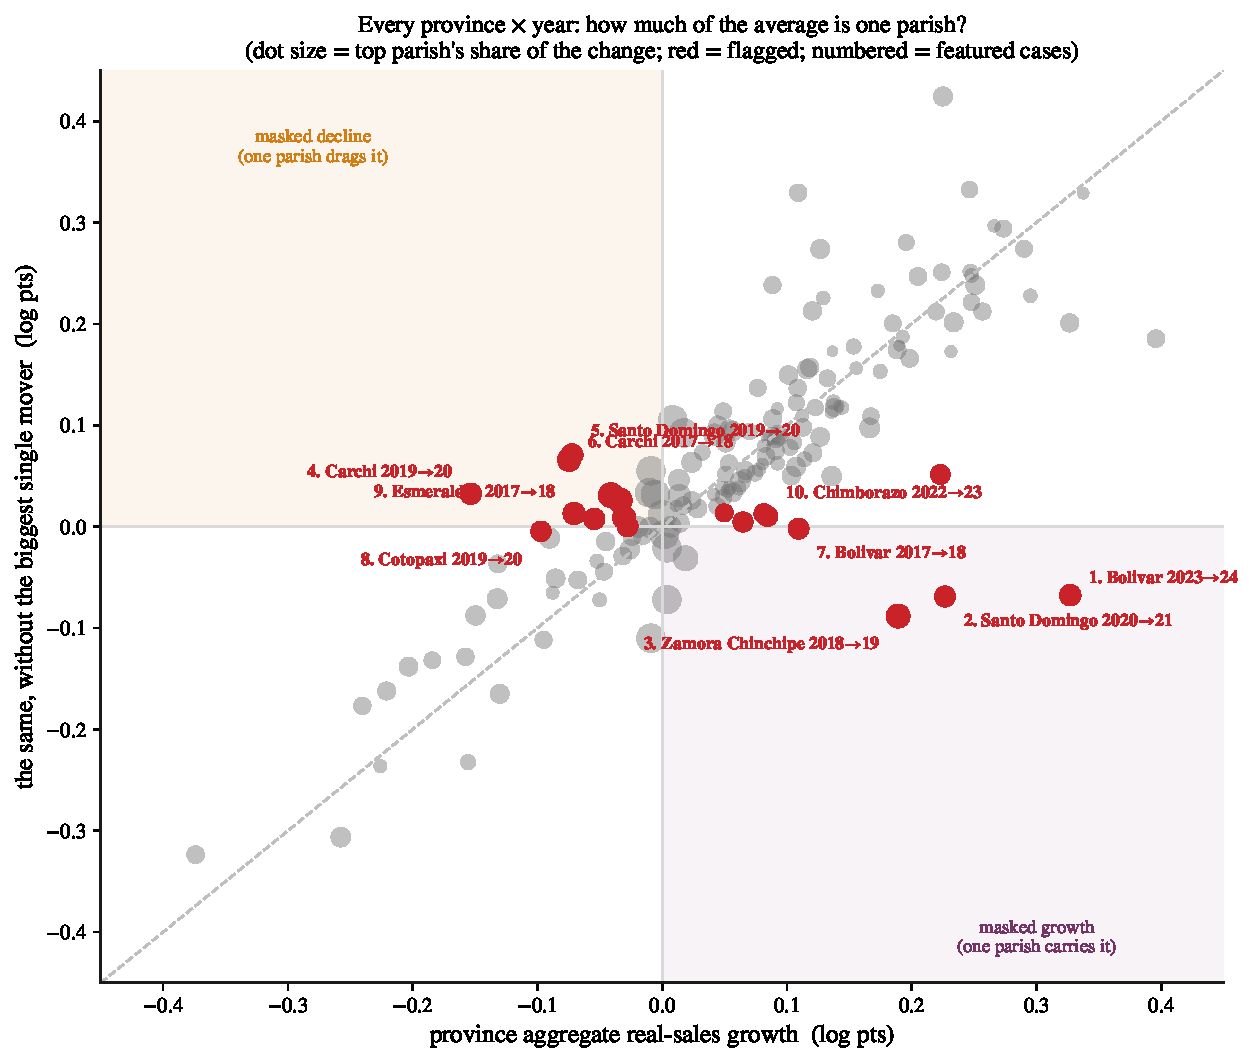
\includegraphics[width=0.7\textwidth]{masked_scan.pdf}
  \caption[Crecimiento agregado frente al crecimiento sin la unidad de mayor variación]{Cada provincia $\times$ paso anual, 2017$\to$2024: crecimiento agregado de las ventas reales $G$ frente al mismo crecimiento sin la unidad de mayor variación, $G_{-1}$. Los puntos rojos fuera de la diagonal son crecimiento enmascarado (sureste) o declive enmascarado (noroeste); los puntos numerados son los casos destacados de la Tabla~\ref{tab:masked}.}
  \label{fig:scan}
\end{figure}

\begin{table}[H]
  \setstretch{0.952}
  \caption[Crecimiento enmascarado y declive enmascarado, casos seleccionados]{Crecimiento enmascarado y declive enmascarado, casos seleccionados (todos los valores en porcentaje).}
  \label{tab:masked}
  \begin{tabular}{|l|l|r|r|r|l|}
    \hline
    \textbf{Provincia} & \textbf{Paso} & $G$ & $G_{-1}$ & $\tilde g$ & \textbf{Explicado por} \\ \hline
    \multicolumn{6}{|l|}{\textit{Crecimiento enmascarado}} \\ \hline
    Bolívar          & 23$\to$24 & $+38.7$ & $-6.5$ & $+6.0$  & Guaranda \\ \hline
    Sto.\ Domingo    & 20$\to$21 & $+25.4$ & $-6.7$ & $+12.3$ & Sto.\ Domingo \\ \hline
    Zamora Ch.       & 18$\to$19 & $+20.8$ & $-8.4$ & $+25.7$ & Los Encuentros \\ \hline
    \multicolumn{6}{|l|}{\textit{Declive enmascarado}} \\ \hline
    Carchi           & 19$\to$20 & $-14.2$ & $+3.3$ & $-13.5$ & Tulcán \\ \hline
    Sto.\ Domingo    & 19$\to$20 & $-7.0$  & $+7.4$ & $-2.7$  & Sto.\ Domingo \\ \hline
    Tungurahua       & 23$\to$24 & $-5.3$  & $+0.8$ & $-1.2$  & Ambato \\ \hline
  \end{tabular}
\end{table}

El caso emblemático es Zamora Chinchipe (Figura~\ref{fig:zamora}), sede de Fruta del Norte, la primera mina de oro a gran escala del Ecuador, en la parroquia de Los Encuentros: alrededor de una docena de empresas formales cuyas ventas reales pasaron de 7.2 millones de dólares y el 7.8~\% de la provincia en 2017 a 1\,150 millones de dólares y el 43~\% de la provincia en 2024. En 2018$\to$2019 la provincia «creció» un 20.8~\%, pero cayó un 8.4~\% sin Los Encuentros, mientras la parroquia \textit{mediana} creció un 25.7~\%; en el año de la COVID, el agregado creció un 377~\% mientras la parroquia mediana se contrajo un 24~\%. La contabilidad en dólares atribuye esencialmente todo el aumento a una parroquia; la contabilidad de Price, que pondera con el criterio de una empresa, un voto, apenas registra cinco empresas. \textit{El desacuerdo entre ambas contabilidades es la huella del enclave}, y el caso simétrico funciona de manera idéntica: el «colapso del 14.2~\%» de Carchi en el año de la COVID es una sola ciudad fronteriza cerrada (Tulcán), sin la cual la provincia agrícola \textit{creció} un 3.3~\%; y dentro de la provincia los dos términos de Price discrepan en el signo, que es precisamente la señal de auditoría. Los casos enmascarados no son errores de los datos: las ventas de la mina son reales. El error consiste en tratar una suma como una descripción, y las dos ponderaciones de la descomposición institucionalizan la auditoría.
\par

\begin{figure}[H]
  \setstretch{0.952}
  \centering
  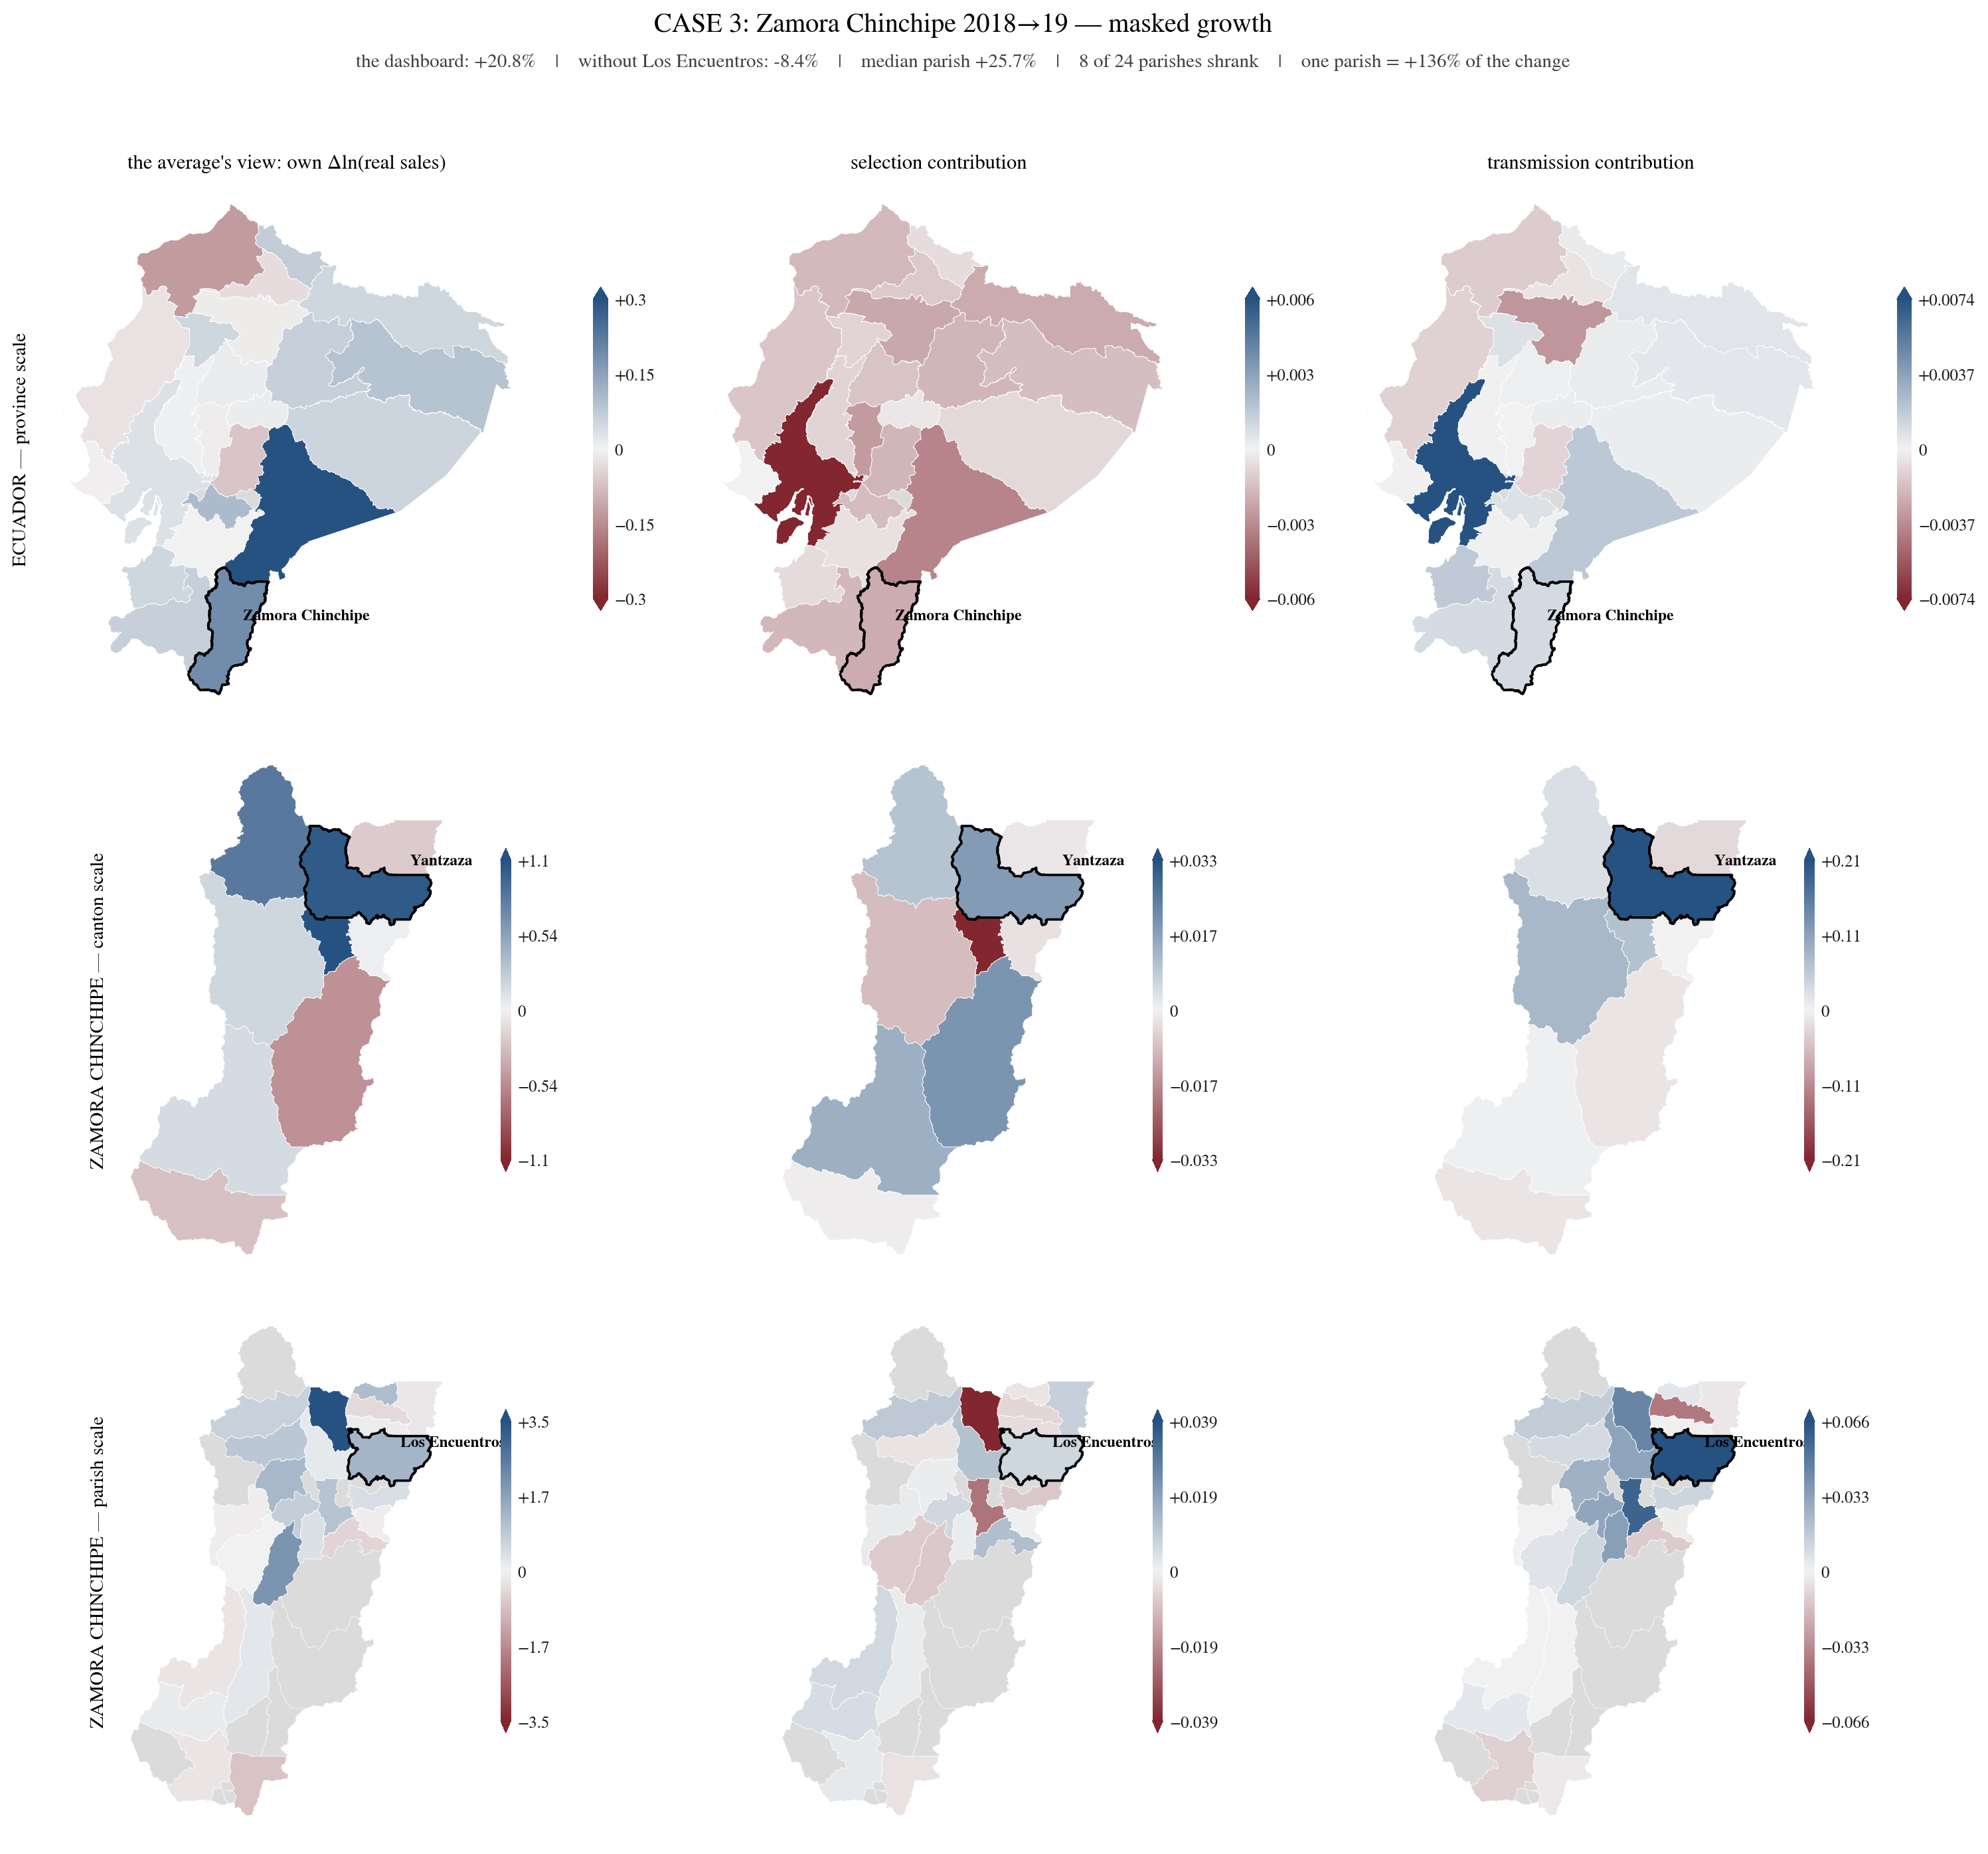
\includegraphics[width=0.75\textwidth]{case_zamora.png}
  \caption[El caso del enclave en tres escalas: Zamora Chinchipe]{El caso del enclave en tres escalas: Zamora Chinchipe, 2018$\to$2019. Las filas van de lo general a lo detallado (el país a escala provincial; la provincia señalada a escala cantonal y parroquial, con la descomposición recalculada dentro de la provincia); las columnas van del promedio a la descomposición (crecimiento de las ventas propias, contribución a la selección, contribución a la transmisión). El mapa nacional muestra un crecimiento sin nada destacable; el acercamiento concentra toda la señal de transmisión en la parroquia de Los Encuentros, mientras la selección a nivel provincial es negativa.}
  \label{fig:zamora}
\end{figure}
\endgroup

% ------------------ ¿LA DIVERSIFICACIÓN COMPRA RESILIENCIA? ------------------
\clearpage
\blank
\tituloapa[¿La diversificación compra resiliencia?]{¿LA DIVERSIFICACIÓN COMPRA RESILIENCIA?}
\begingroup\dobleesp
\subtituloapa{La fragilidad es un fenómeno de ventas; la resiliencia, un fenómeno de entrada}
En el plano sectorial (Figura~\ref{fig:sectormargins}), los dos márgenes de \eqref{eq:margins} dividen el choque de forma asimétrica: las ventas por empresa abarcan 0.58 puntos logarítmicos entre las secciones de la CIIU (alojamiento y comidas $-0.57$, construcción $-0.49$, agua $+0.02$), mientras que el número de empresas abarca solo 0.19, y 17 de 19 secciones siguieron sumando empresas; entre sectores, los dos márgenes presentan una correlación de $-0.27$, débil y, en todo caso, negativa. La fragilidad y la resiliencia son rasgos distintos de un mismo lugar: Quito se ubica a la vez en el percentil 28 de resistencia de las ventas y en el percentil 75 de resistencia de las empresas. Esta asimetría debe leerse con una cautela: el número de empresas proviene del registro, en el que una sociedad sigue activa mientras no suspenda o cancele su RUC, de modo que parte de la estabilidad del margen extensivo refleja esa inercia y no necesariamente actividad.
\par

\begin{figure}[H]
  \setstretch{0.952}
  \centering
  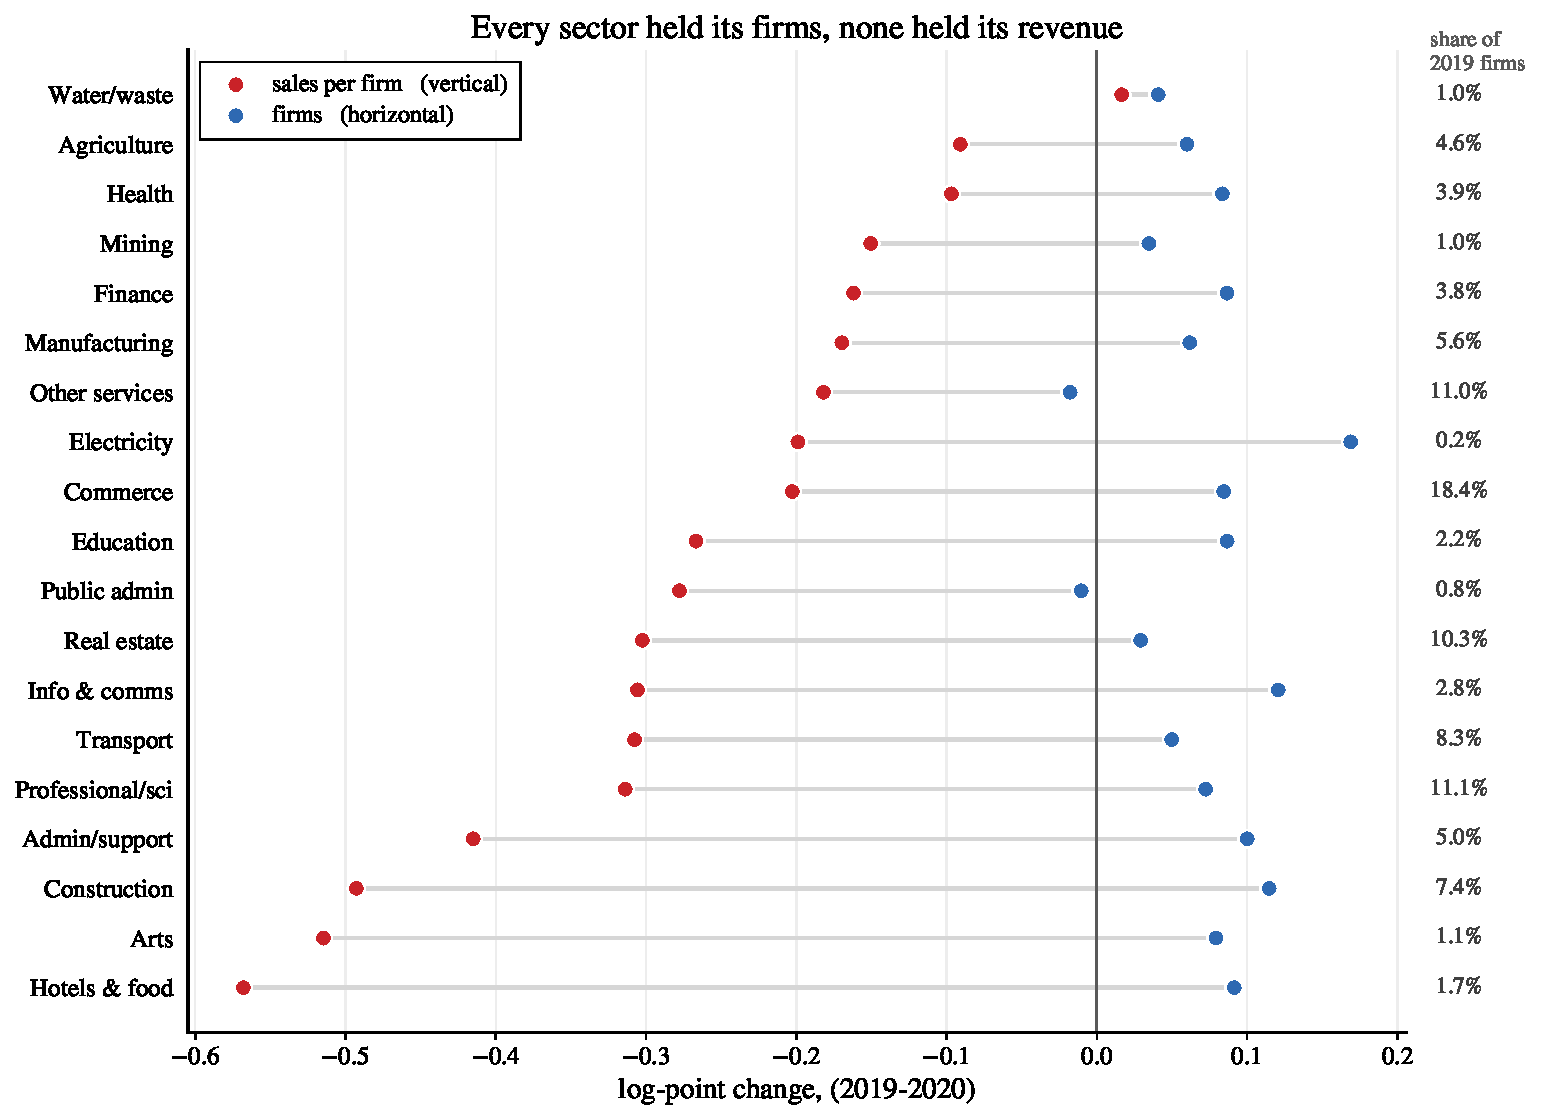
\includegraphics[width=0.85\textwidth]{sector_margins.pdf}
  \caption[Márgenes extensivo e intensivo por sector durante la COVID]{El paso de la COVID por sector: cambio en el número de empresas (margen extensivo) y en las ventas por empresa (margen intensivo), que suman exactamente el crecimiento de las ventas según la Ecuación~\eqref{eq:margins}. Diecisiete de diecinueve sectores siguieron sumando empresas; uno de diecinueve mantuvo sus ventas por empresa.}
  \label{fig:sectormargins}
\end{figure}

La concentración que hace frágiles a los lugares es doble. En el espacio, la provincia mediana registra sus ventas formales en alrededor de cuatro parroquias efectivas (Pastaza y Santo Domingo concentran el 88~\% en una sola parroquia). En lo sectorial, los cráteres más profundos y prolongados de 2020 corresponden todos a lugares de una sola actividad, como los monocultivos turísticos de Puerto Villamil ($-2.1$ puntos logarítmicos, 45 meses por debajo del nivel previo) y Puerto Ayora ($-2.0$, 39 meses), y la exposición a actividades muy afectadas predice el golpe (correlación de rangos de Spearman de alrededor de $-0.5$, controlando por tamaño). Cuando el choque está correlacionado, importa más \textit{qué} actividades tiene un lugar que cuántas.
\par

\subtituloapa{Amplitud y ausencia de caídas extremas}
Si se mide la amplitud de una parroquia como el número efectivo de actividades $D = e^{H}$, donde $H$ es la entropía de Shannon sobre las participaciones de los grupos de actividad de la CIIU rev.~4 en las ventas de una línea base fija de 2019, la Figura~\ref{fig:breadthgroups} ofrece un veredicto en dos partes para las 174 parroquias con al menos 50 empresas. La población y la variable son las del resto del trabajo: sociedades privadas y ventas totales (\texttt{V\_VTX}). Como predictor del \textit{tamaño} de la caída de las ventas, la amplitud casi no aporta: la correlación de rangos es $-0.03$ en la economía completa y $+0.05$ ($p = 0.49$) una vez que se excluyen de ambos lados los cuatro grupos de actividad petrolera (extracción de crudo y de gas, servicios de apoyo y refinación) y las megaceldas, que son las celdas parroquia $\times$ actividad cuyas ventas por contribuyente en 2019 superan el percentil 99 de todas las celdas. Como el extracto solo documenta el rango del número de contribuyentes de cada celda, las ventas se dividen para el límite superior de ese rango, de modo que la cifra es una cota inferior de las ventas por contribuyente y el criterio es conservador. La caída de 2020 fue, en su distribución, un choque de composición sectorial: si a la mezcla de actividades que cada parroquia tenía en 2019 se le aplica el cambio que cada actividad registró en el resto del país, el orden de las caídas previstas reproduce en buena medida el de las observadas (correlación de rangos de $+0.53$), y la amplitud no guarda relación ni con la caída prevista por la mezcla ($-0.08$) ni con la diferencia entre la caída observada y la prevista ($-0.07$; ninguna de las dos es significativa). De las tres ciudades, Quito es la que se aparta: sus ventas cayeron un 20.3~\%, frente al 14.7~\% que su mezcla de actividades anticipaba, mientras que Guayaquil y Cuenca cayeron casi exactamente lo previsto. Lo que sí se observa es que las caídas extremas se concentran en las economías estrechas: la peor caída entre las trece parroquias con al menos 30 actividades efectivas es de $-0.27$ puntos logarítmicos, frente a $-2.15$ entre las otras 161, y el crecimiento de la base empresarial se correlaciona con la amplitud en $+0.29$ ($p = 0.0001$).
\par

\begin{figure}[H]
  \setstretch{0.952}
  \centering
  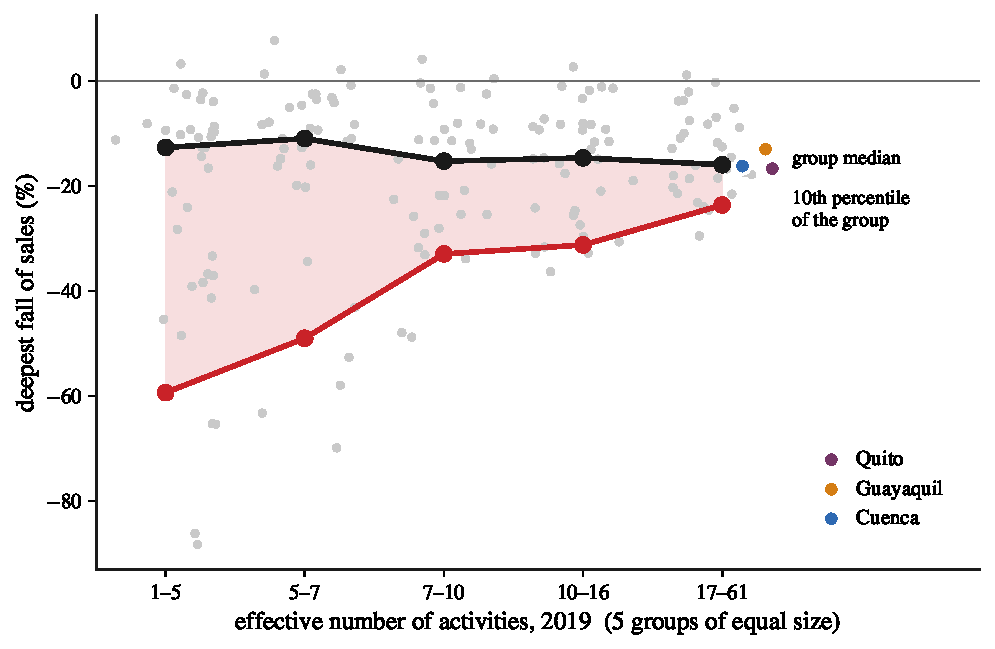
\includegraphics[width=0.85\textwidth]{breadth_groups.pdf}
  \caption[Amplitud y profundidad de la caída, en cinco grupos]{Amplitud y profundidad de la caída de las ventas en las 174 parroquias con al menos 50 empresas (sin petróleo ni megaceldas), ordenadas por amplitud y divididas en cinco grupos del mismo tamaño. Cada punto es una parroquia; las tres ciudades están en el grupo más amplio. La línea negra une la mediana de la caída de cada grupo y la roja, su percentil 10 (la caída que solo una de cada diez parroquias del grupo superó). La mediana es similar en los cinco grupos y el percentil 10 se reduce con la amplitud.}
  \label{fig:breadthgroups}
\end{figure}

La afirmación distributiva (Figuras~\ref{fig:breadthgroups}, \ref{fig:severe} y~\ref{fig:breadthdist}) es la más precisa. Si las 174 parroquias se ordenan por amplitud y se dividen en cinco grupos del mismo tamaño, la mediana de la caída de las ventas es casi la misma en todos: 13, 11, 15, 15 y 16~\%, del grupo más estrecho al más amplio. Lo que cambia es la cola inferior de la distribución. El percentil 10 de cada grupo, es decir, la caída que solo una de cada diez de sus parroquias superó, pasa de 59~\% en el grupo más estrecho a 49, 33, 31 y 24~\% en los siguientes, y la proporción de parroquias que perdió más del 30~\% de sus ventas baja de 34~\% a 20, 18, 14 y 0~\%. El resultado no depende de haber elegido cinco grupos: la prueba de Brown--Forsythe rechaza la igualdad de dispersiones con dos, tres, cuatro y cinco grupos ($p$ entre $0.0006$ y $0.013$), y sin grupo alguno, una regresión cuantílica sobre el logaritmo de la amplitud da una pendiente de $+0.171$ ($p = 0.0003$) en el percentil 10 y de $-0.020$ ($p = 0.29$) en la mediana: la caída ajustada en el percentil 10 pasa de 49~\% con tres actividades efectivas a 24~\% con treinta, mientras que la mediana ajustada va de 12~\% a 16~\%. La Figura~\ref{fig:breadthdist} muestra la forma completa de las distribuciones con tres grupos: las medianas de la caída casi coinciden ($-0.13$, $-0.15$ y $-0.16$ puntos logarítmicos, del grupo más estrecho al más amplio), mientras que su desviación estándar se reduce de $0.42$ a $0.24$ y $0.10$, y la cola hacia las caídas grandes, visible en los dos grupos más estrechos, no aparece en el más amplio. Las parroquias más amplias no sufrieron un daño por empresa menor sino, en todo caso, algo mayor: la correlación de rangos entre la amplitud y el cambio de las ventas por empresa es de $-0.17$ ($p = 0.03$). En el margen extensivo, el 97~\% de las parroquias del grupo más amplio sumó empresas, frente al 74~\% del más estrecho, pero la dispersión del crecimiento de las empresas no se reduce de forma robusta con la amplitud (la misma prueba da $p = 0.09$ con tres grupos y $p = 0.11$ con cinco), de modo que la afirmación se limita a las ventas. La amplitud no se asocia con un choque promedio más pequeño, sino con la ausencia de caídas extremas. Es el patrón que predice el argumento de cartera de la literatura sobre variedad y resiliencia regional \parencite{martin2015,frenken2007}, pero el párrafo siguiente explica por qué estos datos no permiten atribuirlo a la diversificación.
\par

\begin{figure}[H]
  \setstretch{0.952}
  \centering
  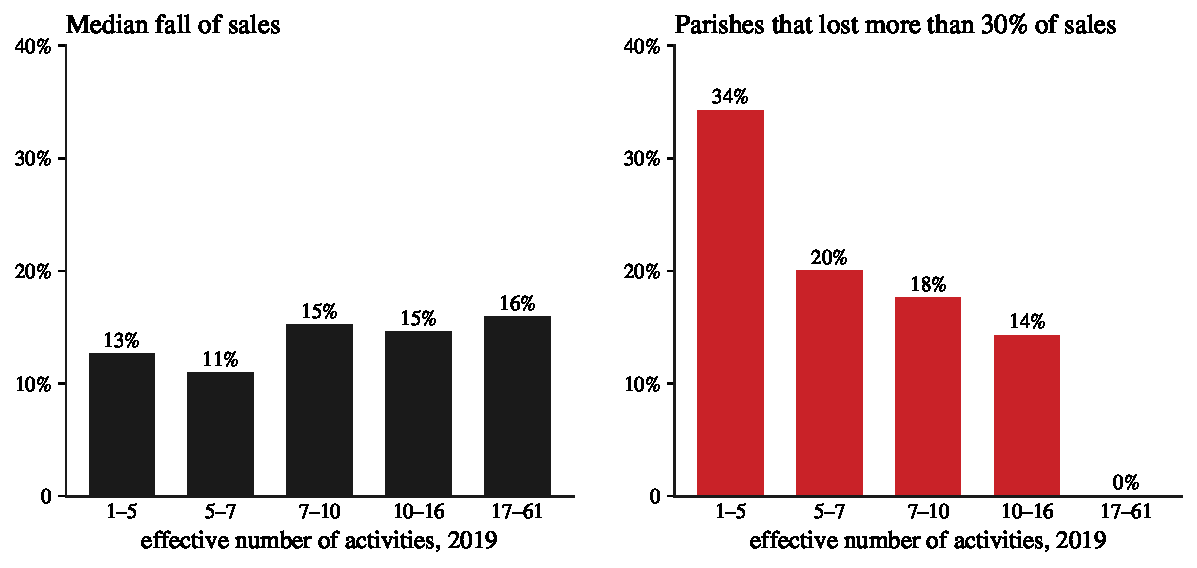
\includegraphics[width=\textwidth]{typical_vs_severe.pdf}
  \caption[Mediana de la caída y caídas severas por grupo de amplitud]{Los mismos cinco grupos en dos indicadores. Izquierda: mediana de la caída de las ventas. Derecha: proporción de las parroquias del grupo que perdió más del 30~\% de sus ventas.}
  \label{fig:severe}
\end{figure}

\begin{figure}[H]
  \setstretch{0.952}
  \centering
  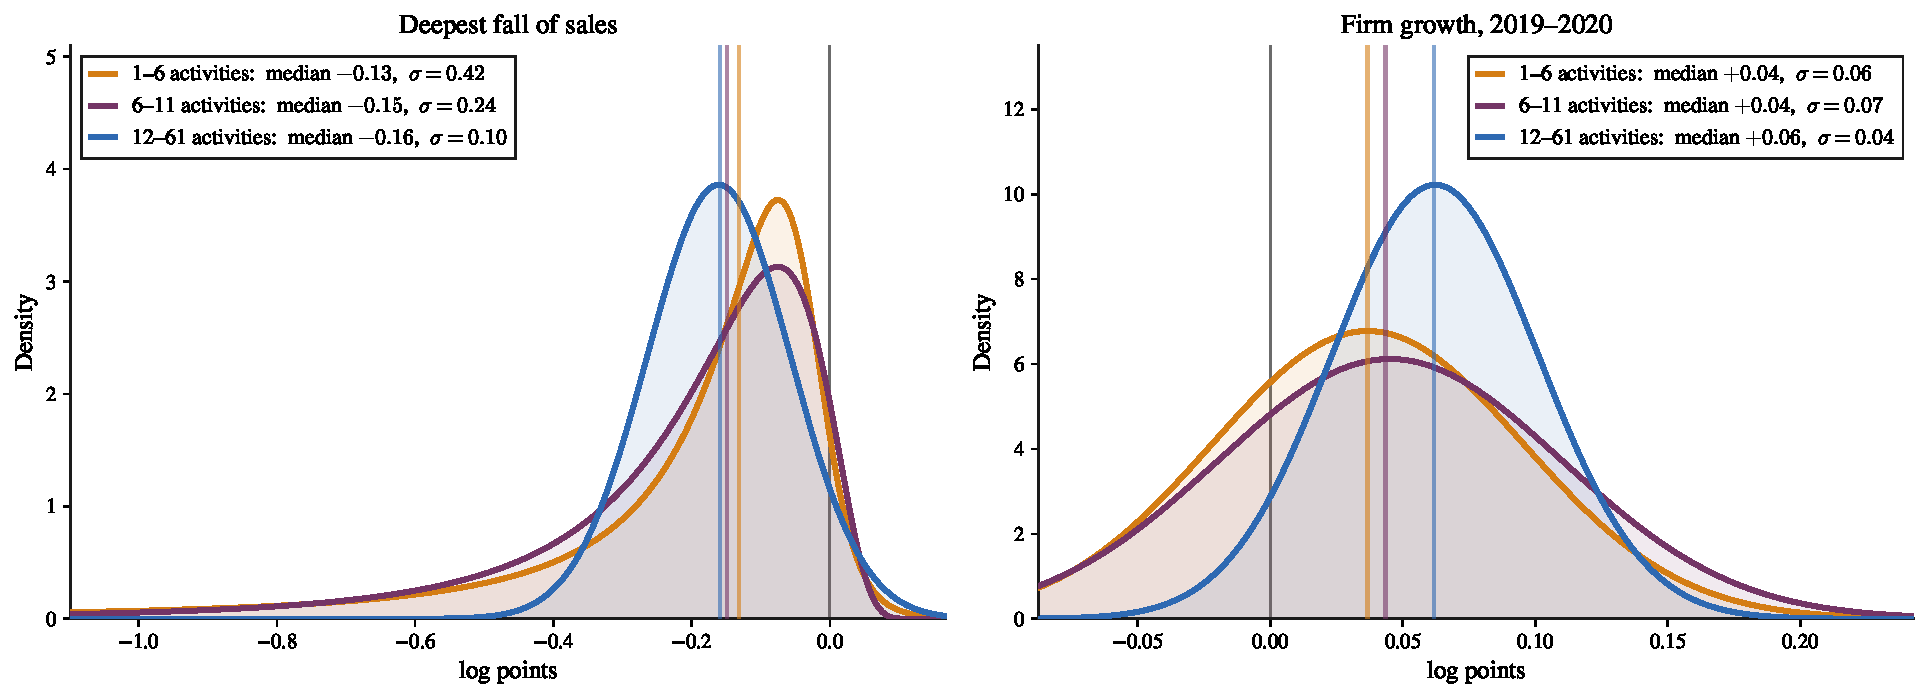
\includegraphics[width=\textwidth]{breadth_distributions.pdf}
  \caption[Distribuciones de la caída de las ventas y del crecimiento de las empresas por amplitud]{Distribuciones ajustadas, en puntos logarítmicos, de la caída de las ventas (izquierda) y del crecimiento del número de empresas en 2019$\to$2020 (derecha), para las 174 parroquias divididas por su amplitud en tres grupos del mismo tamaño (58 parroquias cada uno). Cada curva es un ajuste continuo (una $t$ de Student asimétrica cuando supera a la normal en al menos diez puntos del criterio de Akaike; la normal en caso contrario) y la línea vertical del mismo color marca la mediana del grupo; $\sigma$ es la desviación estándar. Los ejes abarcan del percentil 3 al 99.5 de cada variable, con lo que quedan fuera tres parroquias en el panel izquierdo y cuatro en el derecho. En las ventas, las medianas casi coinciden y la cola hacia las caídas grandes desaparece en el grupo más amplio.}
  \label{fig:breadthdist}
\end{figure}

Un factor de confusión acota la afirmación: en el Ecuador, amplitud y tamaño van juntos (correlación de $+0.65$). Hay además una razón mecánica para esperar el patrón aun sin efecto alguno de la diversificación: el total de una parroquia grande suma miles de empresas cuyas variaciones individuales se compensan, de modo que fluctúa menos que el de una parroquia con pocas empresas; y la comparación entre la peor caída de un grupo de 13 parroquias y la de un grupo de 161 favorece por construcción al grupo pequeño. Tres comprobaciones miden cuánto queda después de esas objeciones. (a)~\textit{Una prueba de permutación.} Si se extraen al azar 20\,000 grupos de 13 parroquias, solo el 1.4~\% tiene una peor caída tan leve como la del grupo amplio, de modo que el resultado no es fruto del azar; si los grupos se extraen únicamente de las 39 parroquias más grandes, la proporción sube al 4.4~\%, y en la economía completa (nueve parroquias amplias) las cifras son 4.3~\% y 6.3~\%. Frente a parroquias de su mismo tamaño, la ventaja de las amplias es, por tanto, marginal. (b)~\textit{Amplitud y tamaño en la misma regresión.} Con el logaritmo del número de empresas y el de la amplitud como regresores, ninguno de los dos se asocia con la profundidad promedio de la caída de las ventas; en el extremo malo de la distribución (regresión cuantílica en el percentil 10) y en la dispersión de los resultados, la variable que conserva una asociación significativa es la amplitud y no el tamaño. En el crecimiento del número de empresas ocurre lo contrario: es el tamaño el que se asocia con una menor dispersión, y al descontarlo no queda relación alguna con la amplitud (correlación de $+0.05$). Como ambas variables están muy correlacionadas, estos signos son indicios y no magnitudes. (c)~\textit{Otra contracción.} Entre 2015 y 2016, con la caída del precio del petróleo y el terremoto de abril de 2016, las ventas reales de las sociedades privadas cayeron 0.09 puntos logarítmicos. Con las mismas parroquias y la amplitud medida en 2015, el patrón tiene la misma dirección (correlación de $-0.11$, no significativa, con el cambio de las ventas; peor caída de $-0.14$ entre las siete parroquias amplias frente a $-0.86$ en el resto), pero un grupo aleatorio de siete parroquias lo iguala el 12.7~\% de las veces: la comprobación no contradice el resultado de 2020 ni lo confirma. Esta sección describe, por tanto, una asociación y no un mecanismo, y no permite concluir que la diversificación proteja por sí sola. La afirmación defendible es que, en la caída de las ventas, las economías amplias evitaron los peores desenlaces, y que esa ventaja se reduce a un margen estrecho cuando se las compara con parroquias de su mismo tamaño; en el número de empresas, lo que cuenta es el tamaño. El resultado se mantiene como preliminar.
\par
\endgroup

% ----------------------------- ROBUSTEZ -----------------------------
\clearpage
\blank
\tituloapa[Robustez]{ROBUSTEZ}
\begingroup\dobleesp
\vspace{6pt}
Las variantes de robustez se fijaron de antemano en tres dimensiones (rasgo, unidad de análisis y ventana temporal), a las que se añadieron los tratamientos de valores atípicos y de validez de los datos. Las variantes ejecutadas son: (1)~el rasgo y la vía: población (logaritmo de las ventas, con su partición en tamaño y ventas por empresa), ingreso (nivel de ventas) y densidad (número de empresas), en las secciones de resultados; (2)~la unidad de análisis: parroquias, con la selección dividida entre cantones y entre provincias, y el análisis por cantón y por provincia en los casos de crecimiento enmascarado; (3)~la ventana temporal: pasos anuales consecutivos, ventanas trimestrales y 72 ventanas móviles de doce meses; (4)~los valores atípicos de la aptitud: sin ajuste, winsorización y recorte en los percentiles 1 y 99; (5)~el umbral de validez de las ventas anuales: 1, 1\,000 y 100\,000 dólares; (6)~la exclusión de Quito y Guayaquil en las distribuciones no ponderadas; (7)~la certificación numérica de la identidad en todas las unidades, escalas y ventanas; y (8)~cuatro decisiones de preparación de datos: la regla de sobrevivencia, la comparación de los mismos meses en ambos extremos, la inclusión de las exportaciones en las ventas y la definición del número de empresas. Esta sección reporta las variantes (4), (5), (7) y (8); las demás aparecen en las secciones correspondientes.
\par\vspace{6pt}
La selección es una covarianza entre una variable moderada y una desbocada: el rasgo tiene una asimetría de $+0.14$ y una curtosis en exceso de $-0.44$, mientras que el cociente bruto de aptitud tiene una asimetría de $+5.0$, una curtosis de $+45$ y un máximo de $17.6\times$. Una variable con colas tan pesadas podría, en principio, permitir que unas pocas parroquias explosivas dictaran el resultado principal. No ocurre así (Tabla~\ref{tab:robust}): winsorizar o recortar la aptitud en sus percentiles 1 y 99 modifica la selección en menos de un 3~\%, y variar el umbral de validez de los datos de 1 a 100\,000 dólares anuales (cuyo último paso excluye un tercio de todas las parroquias) mantiene la selección de la ventana completa en $[-0.026, -0.028]$ en todo momento. La inversión de 2019$\to$2020 tampoco proviene de valores atípicos: con la aptitud winsorizada o recortada vale $+0.0346$ y $+0.0339$, frente a $+0.0342$; como se muestra más abajo, de lo que depende es de la definición del número de empresas.
\par

\begin{table}[H]
  \setstretch{0.952}
  \caption[Prueba de valores atípicos y umbrales de validez]{La prueba de valores atípicos: selección de la vía de población en la ventana completa bajo distintos tratamientos de valores atípicos y umbrales de validez de los datos.}
  \label{tab:robust}
  \begin{tabular}{|l|r|r|r|}
    \hline
    \textbf{Variante} & \textbf{Selección} $S^{p}$ & \textbf{Entre prov.} & \textbf{Transmisión} $T^{p}$ \\ \hline
    Sin ajuste                        & $-0.0270$ & $-0.0227$ & $+0.0496$ \\ \hline
    Winsorizado p1/p99                & $-0.0265$ & $-0.0224$ & $+0.0494$ \\ \hline
    Recortado p1/p99                  & $-0.0262$ & $-0.0221$ & $+0.0492$ \\ \hline
    Umbral US\$1 (859 parr.)          & $-0.0263$ & $-0.0228$ & $+0.0501$ \\ \hline
    Umbral US\$1\,000 (804 parr.)     & $-0.0270$ & $-0.0227$ & $+0.0496$ \\ \hline
    Umbral US\$100\,000 (576 parr.)   & $-0.0276$ & $-0.0223$ & $+0.0485$ \\ \hline
  \end{tabular}
\end{table}

La especificación base adoptada conserva la aptitud sin ajustar (la cola pesada es una señal real, y los pesos de participación de empresas ya limitan su influencia), aplica solo el umbral de 1\,000 dólares como exclusión por validez de los datos y nunca excluye a Quito ni a Guayaquil: su influencia proviene de su participación de empresas y no de un crecimiento extremo, y constituyen el contenido del término entre provincias, no una contaminación. Dos certificaciones adicionales cierran el caso: el residuo de la identidad es del orden de $10^{-17}$ en todas las ventanas exportadas, y los gráficos de reconstrucción en todos los niveles y vías se sitúan sobre la diagonal de identidad con $R^2 = 1.0000$. La selección negativa es estructural.
\par\vspace{6pt}
Tres decisiones de preparación de datos se sometieron a prueba tras las revisiones de los dos primeros avances, reutilizando el mismo controlador y el mismo motor y cambiando únicamente la tabla parroquia $\times$ mes que entra en ellos (Tabla~\ref{tab:datos}; programa \texttt{robustness\_data\_decisions.py} del repositorio). (a)~\textit{Las parroquias sobrevivientes.} Incluir en el promedio nacional a las parroquias válidas en un solo extremo cambia el cambio del rasgo 2017$\to$2023 de $+0.0226$ a $+0.0207$ por año, y el de cada paso anual en menos de $0.009$; la contribución de las entradas y salidas es del orden de una décima del cambio y no altera ningún signo. (b)~\textit{Los mismos meses en ambos extremos.} Como el panel de 2024 carece de noviembre, el paso 2022$\to$2023 se recalculó con los mismos once meses: la selección pasa de $-0.0183$ a $-0.0271$ y el término entre provincias de $-0.0179$ a $-0.0266$, lo que muestra que un paso anual no debe compararse entre bases de meses distintas. Con esa regla, el paso 2023$\to$2024 da un cambio de $-0.0055$, con selección $-0.0075$ (entre provincias $+0.0160$, entre cantones $-0.0182$, entre parroquias $-0.0053$) y transmisión $+0.0020$, y la ventana 2017$\to$2024 reproduce la estructura de 2017$\to$2023: selección $-0.0259$ (entre provincias $-0.0180$, entre cantones $-0.0107$, entre parroquias $+0.0027$) y transmisión $+0.0439$. El paso 2023$\to$2024 se calcula por primera vez en esta versión y se reporta como preliminar. (c)~\textit{Las exportaciones.} Las ventas del trabajo incluyen las exportaciones, que representan entre el 10 y el 13~\% de las ventas de las sociedades privadas en 2017--2023. Al repetir la descomposición con las ventas internas (\texttt{V\_VTX} menos \texttt{V\_X}), la ventana 2017$\to$2023 da una selección de $-0.0267$ (frente a $-0.0270$), un término entre provincias de $-0.0226$ ($-0.0227$) y una transmisión de $+0.0480$ ($+0.0496$); en ningún paso anual la selección cambia en más de $0.0006$, y la inversión de 2019$\to$2020 se mantiene ($+0.0345$ frente a $+0.0342$). La única diferencia apreciable está en la transmisión de ese paso ($-0.170$ frente a $-0.155$): las ventas internas cayeron más que las exportaciones.
\par

\begin{table}[H]
  \setstretch{0.952}
  \caption[La regla de los mismos meses]{La regla de los mismos meses: vía de población con doce meses y con los once meses presentes en 2024 (enero a octubre y diciembre) en ambos extremos (puntos logarítmicos por año).}
  \label{tab:datos}
  \small
  \begin{tabular}{|l|l|r|r|r|r|r|r|}
    \hline
    \textbf{Meses} & \textbf{Ventana} & $\gamma^{p}$ & $S^{p}$ & \textbf{prov.} & \textbf{cantón} & \textbf{parroq.} & $T^{p}$ \\ \hline
    12 & 2022$\to$23 & $+0.0259$ & $-0.0183$ & $-0.0179$ & $-0.0125$ & $+0.0121$ & $+0.0442$ \\ \hline
    11 & 2022$\to$23 & $+0.0207$ & $-0.0271$ & $-0.0266$ & $-0.0142$ & $+0.0136$ & $+0.0478$ \\ \hline
    11 & 2023$\to$24 & $-0.0055$ & $-0.0075$ & $+0.0160$ & $-0.0182$ & $-0.0053$ & $+0.0020$ \\ \hline
    12 & 2017$\to$23 & $+0.0226$ & $-0.0270$ & $-0.0227$ & $-0.0086$ & $+0.0043$ & $+0.0496$ \\ \hline
    11 & 2017$\to$24 & $+0.0180$ & $-0.0259$ & $-0.0180$ & $-0.0107$ & $+0.0027$ & $+0.0439$ \\ \hline
  \end{tabular}
\end{table}

\subtituloapa{Otros objetos de estudio}
Dos ejercicios adicionales no son pruebas de robustez, porque no modifican una decisión de preparación de los datos, sino el sujeto del análisis; sus resultados no son comparables con los de este trabajo y no los vuelven provisionales. El primero es la inclusión de los demás tipos de contribuyente: como se muestra en la sección de Datos, al sumar a las personas naturales estas aportan el 91.6~\% de las unidades con ventas por unidad 37 veces menores, y la descomposición pasa a describirlas a ellas y no a las sociedades. El segundo es el catastro completo de sociedades activas, que cuenta también a las sociedades situadas en celdas sin ventas declaradas, de las que no se observa el rasgo (Tabla~\ref{tab:registro}; mismo programa). En la ventana 2017$\to$2023 el catastro muestra el mismo patrón que la población del estudio: selección $-0.0251$ frente a $-0.0270$, término entre provincias $-0.0220$ frente a $-0.0227$ (88 y 84~\% de la selección), entre cantones $-0.0088$ frente a $-0.0086$, entre parroquias $+0.0056$ frente a $+0.0043$ y transmisión $+0.0515$ frente a $+0.0496$. En los pasos anuales no: en el catastro la selección es negativa en los seis pasos, pero casi nula en 2019$\to$2020 ($-0.0021$) y en 2020$\to$2021 ($-0.0003$), y mayor en 2022$\to$2023 ($-0.0436$ frente a $-0.0183$). La sección sobre la inversión explica de dónde proviene la diferencia: en 2020 se concentró la actividad con ventas declaradas, no el domicilio de las sociedades activas. Ambos ejercicios se documentan para delimitar el alcance de los resultados, que se refieren a las sociedades privadas en actividades con ventas declaradas.
\par

\begin{table}[H]
  \setstretch{0.952}
  \caption[El mismo cálculo sobre el catastro completo de sociedades activas]{El mismo cálculo sobre dos objetos distintos, vía de población (puntos logarítmicos por año). Principal: la población del estudio, sociedades activas en las celdas con ventas declaradas. Todas: el catastro completo de sociedades activas, incluidas las de celdas sin ventas declaradas. Las ventas son las mismas. La columna «todas» no es una prueba de robustez de la columna «principal».}
  \label{tab:registro}
  \small
  \begin{tabular}{|l|r|r|r|r|r|r|}
    \hline
    & \multicolumn{2}{c|}{\textbf{Selección} $S^{p}$} & \multicolumn{2}{c|}{\textbf{Entre prov.}} & \multicolumn{2}{c|}{\textbf{Transmisión} $T^{p}$} \\ \hline
    \textbf{Paso} & \textbf{principal} & \textbf{todas} & \textbf{principal} & \textbf{todas} & \textbf{principal} & \textbf{todas} \\ \hline
    2017$\to$18 & $-0.0451$ & $-0.0205$ & $-0.0296$ & $-0.0178$ & $+0.0641$ & $+0.0672$ \\ \hline
    2018$\to$19 & $-0.0597$ & $-0.0402$ & $-0.0508$ & $-0.0425$ & $+0.0139$ & $+0.0145$ \\ \hline
    2019$\to$20 & $\mathbf{+0.0342}$ & $\mathbf{-0.0021}$ & $+0.0149$ & $-0.0026$ & $-0.1552$ & $-0.1582$ \\ \hline
    2020$\to$21 & $-0.0346$ & $-0.0003$ & $-0.0223$ & $-0.0048$ & $+0.2124$ & $+0.2130$ \\ \hline
    2021$\to$22 & $-0.0338$ & $-0.0330$ & $-0.0286$ & $-0.0298$ & $+0.1129$ & $+0.1169$ \\ \hline
    2022$\to$23 & $-0.0183$ & $-0.0436$ & $-0.0179$ & $-0.0306$ & $+0.0442$ & $+0.0480$ \\ \hline
    2017$\to$23 & $-0.0270$ & $-0.0251$ & $-0.0227$ & $-0.0220$ & $+0.0496$ & $+0.0515$ \\ \hline
  \end{tabular}
\end{table}
\par
\endgroup

% ---------------------------- LIMITACIONES ----------------------------
\clearpage
\blank
\tituloapa[Limitaciones]{LIMITACIONES}
\begingroup\dobleesp
\vspace{6pt}
Nueve límites acompañan a cada cifra. (1)~El número de empresas corresponde a stocks de contribuyentes activos del registro en las celdas con declaración, no a identidades de empresas ni al número de sociedades que declararon (en una celda con declaración puede haber sociedades activas que no declararon ese mes); una sociedad permanece activa en el registro mientras no suspenda o cancele su RUC, por lo que el stock puede sobrestimar el número de empresas en operación y suavizar sus caídas. Solo se identifica la entrada neta, y el ingreso de las empresas entrantes se acota en lugar de medirse; al regresar el cambio de las ventas por empresa sobre la tasa de entrada, el ingreso del entrante neto marginal queda acotado en un 30~\% o menos del ingreso de una empresa promedio. (2)~La descomposición cubre solo a las unidades sobrevivientes, sin términos de nacimiento ni de muerte, en concordancia con el marco de referencia. (3)~Las ventas se registran en el domicilio fiscal, de modo que la lente del enclave y la advertencia sobre el sesgo de las sedes metropolitanas son dos caras de la misma moneda; eliminar las celdas de actividad gigantes elimina sus ventas directas pero no su demanda indirecta, por lo que esos ejercicios acotan los contrafactuales en lugar de identificarlos. (4)~La economía informal, que representa la mayor parte del empleo ecuatoriano, es invisible por construcción; toda afirmación concierne al margen formal. (5)~El deflactor es constante dentro de cada año, lo que se cancela por completo en la selección pero escala la transmisión. (6)~La ubicación es el domicilio tributario según el RUC vigente a la fecha del corte y no el lugar físico de la actividad, y la geografía de cada contribuyente es constante en toda la serie: los cambios de domicilio o de actividad ocurridos dentro del período no se observan, de modo que la reasignación medida es la que resulta de la entrada neta de empresas y del crecimiento de sus ventas, no de la migración de contribuyentes. (7)~Las dos fuentes delimitan el sector privado con categorías distintas (\texttt{SDD\_NO\_PUB} en las ventas; subtipo «Sector privado» en los conteos), por lo que las ventas podrían incluir organizaciones de la economía popular y solidaria y organismos internacionales que los conteos excluyen; la asimetría es pequeña en número de entidades, pero no se ha cuantificado. (8)~La medida es la venta bruta declarada, no el valor agregado: dos parroquias con el mismo valor agregado pueden declarar ventas muy distintas según la longitud de sus cadenas de intermediación, y ningún resultado debe leerse como una afirmación sobre producto o ingreso. (9)~El rasgo de la vía de población es el total de ventas de la parroquia, que está dominado por su tamaño en número de empresas (correlación ponderada de $0.97$), y los totales de las vías de ingreso y de densidad están dominados por dos parroquias; por eso la selección se lee como dispersión hacia lugares más pequeños, y la partición del rasgo y la advertencia sobre los pesos forman parte de la lectura de cada cifra. Ninguno de estos límites afecta a la contabilidad en sí, que es exacta; delimitan aquello de lo que trata la contabilidad.
\par
\endgroup

% --------------------------- CONCLUSIONES ---------------------------
\clearpage
\blankdoble
\tituloapa[Conclusiones e hipótesis de política]{CONCLUSIONES E HIPÓTESIS DE POLÍTICA}
\begingroup\dobleesp
\vspace{6pt}
La expansión del sector privado formal del Ecuador entre 2017 y 2023, medida en las ventas declaradas por las sociedades privadas, es un fenómeno horizontal con un costo vertical: las empresas se multiplicaron por 1.74 mientras las ventas reales crecieron por 1.30, y los dos márgenes cuentan habitualmente historias opuestas sobre un mismo lugar. La adaptación de la descomposición de Price de \textcite{kemp2025} al sector empresarial convierte esa observación en una contabilidad exacta y multiescala, verificada a mano en un cantón y a precisión de máquina en todos. Sus hallazgos descriptivos centrales son tres, y son el mismo hallazgo visto en tres escalas. El stock de sociedades privadas \textit{sí} se está dispersando espacialmente hacia los lugares más pequeños: sobre todo entre provincias (84~\% de la selección) y en menor medida entre cantones dentro de las provincias (un tercio, con el mismo signo), mientras que entre parroquias dentro de los cantones el componente es pequeño y ha cambiado de signo desde 2021. El proceso es lento (la participación de Quito y Guayaquil en el stock de empresas pasó de 56.5~\% a 52.9~\% en seis años), corresponde en un 88~\% al tamaño de los lugares y no a sus ventas por empresa, y en el único año de contracción de la muestra se invirtió hacia los centros: se concentró la actividad con ventas declaradas, mientras el catastro de sociedades activas siguió creciendo a tasas similares en todas partes. La caída de las ventas por empresa, en cambio, ocurrió dentro de los lugares y no por reasignación entre ellos. Los promedios certifican crecimiento que una sola mina, una sola ciudad fronteriza o una sola ciudad produjeron por sí solas, y certifican calma en provincias donde la mitad del mapa está colapsando: aproximadamente una de cada nueve cifras provinciales de crecimiento. Y la ausencia de caídas catastróficas en 2020 se asocia con la amplitud sectorial, una asociación que no se traduce en una caída promedio distinta, que se reduce a un margen estrecho cuando las parroquias amplias se comparan con otras de su mismo tamaño y que no puede leerse como un efecto protector de la diversificación por sí sola.
\par\vspace{6pt}
Estos patrones permiten formular cinco hipótesis de política. Son hipótesis y no recomendaciones probadas: el diseño de este trabajo es descriptivo, no identifica causas y no evalúa la eficacia de ningún instrumento; ponerlas a prueba requiere diseños de identificación que quedan fuera de su alcance. \textit{Primera: la escala importa para el diseño.} La reasignación es mucho mayor entre provincias que entre cantones, y casi nula entre parroquias dentro de un cantón (la ley de Gibrat se cumple aproximadamente a escala local); un instrumento que busque redistribuir la actividad formal tendría que evaluarse en la escala en la que la reasignación efectivamente ocurre. \textit{Segunda: la convergencia observada es lenta.} La participación de las dos áreas metropolitanas en el stock de empresas se redujo 3.5 puntos porcentuales en seis años, y la descomposición ofrece una velocidad de referencia frente a la cual un cambio de tendencia sería detectable en pocos años de ventanas mensuales. \textit{Tercera: la dispersión podría ser procíclica.} En el único paso de contracción de la muestra la dispersión se interrumpió: el stock de sociedades en actividades con ventas declaradas creció menos en la periferia que en los centros, aunque el stock de todas las sociedades activas creció al mismo ritmo en todas partes; si el patrón se repitiera en otras contracciones, la serie mensual de selección serviría como indicador de reconcentración, algo que solo podría establecerse con más episodios. \textit{Cuarta: la escala de evaluación condiciona lo que se observa.} Como la mayor parte de la selección vive entre provincias, una evaluación basada en promedios parroquiales o cantonales detectaría solo una fracción de ella. \textit{Quinta: los agregados provinciales de ventas requieren auditoría de composición.} El detector de tres números muestra que una de cada nueve cifras provinciales de crecimiento corresponde, en primera aproximación, a una sola parroquia, lo que es relevante allí donde esas cifras alimentan decisiones (regalías, transferencias, evaluaciones de desempeño). Todo ello puede calcularse cada mes a partir de dos columnas que el Estado ya posee, un número de empresas y un total de ventas por lugar; la descomposición es lo que convierte esas dos columnas en una contabilidad de lugares con nombre propio.
\par\vspace{6pt}
Conviene, por último, separar lo que está establecido de lo que sigue siendo preliminar. Está establecido lo que la contabilidad garantiza y lo que las pruebas de robustez confirman: la identidad exacta en todas las escalas y su partición exacta por rasgo; el signo negativo de la selección, su concentración entre provincias y su composición (tamaño, no ventas por empresa); el signo positivo y la mayor magnitud de la transmisión; y la estabilidad de estas tres propiedades frente a los valores atípicos, los umbrales de validez, la regla de sobrevivencia, la base de meses y la inclusión de las exportaciones en las ventas. La inversión de 2019$\to$2020 es un resultado de la población del estudio, se mantiene ante el tratamiento de los valores atípicos y la exclusión de las exportaciones, y su alcance es el de esa población y el de un solo episodio de contracción: describe la actividad con ventas declaradas y no el catastro de sociedades activas. Siguen siendo preliminares la magnitud de los pasos anuales individuales; el cambio de régimen de la escala parroquial posterior a 2021; el paso 2023$\to$2024, calculado por primera vez en esta versión con once meses; la asociación entre diversificación y ausencia de desastres, que solo se separa del tamaño de forma marginal; y las cinco hipótesis de política, que son hipótesis. Quedan abiertas tres preguntas que estos datos no pueden responder: cuántas sociedades de cada celda declaran efectivamente, porque los conteos son agrupados; si el aumento del stock corresponde a sociedades nuevas, a reactivaciones o a cambios de domicilio; y si la interrupción de la dispersión observada en 2020 se repite en otras contracciones.
\par
\endgroup

% --------------------------- AGRADECIMIENTOS ---------------------------
\clearpage
\blank
\tituloapa[Agradecimientos]{AGRADECIMIENTOS}
\begingroup\dobleesp
\vspace{6pt}
El autor agradece a Pablo Astudillo Estévez, tutor de esta tesis, por su supervisión y por sus observaciones a lo largo del trabajo; a Jordan Kemp, por su mentoría y por el motor de descomposición que este trabajo utiliza; y a su familia, en especial a su madre, por su apoyo constante. Esta investigación se llevó a cabo en el marco del programa Emergent Political Economies.
\par
\endgroup

% ---------------------- REFERENCIAS BIBLIOGRÁFICAS ----------------------
% La lista se genera automáticamente a partir de bib/tesis.bib.
% \nocite conserva las dos obras que la lista IEEE original incluía sin citarlas.
\nocite{foster2001,bettencourt2007}
\clearpage
\blank
\tituloapa[Referencias bibliográficas]{REFERENCIAS BIBLIOGRÁFICAS}
\printbibliography[heading=sinTitulo]

% ------------------------------ ANEXOS ------------------------------
\clearpage
\blank
\tituloapa[Anexo A: Diccionario y muestra de las fuentes del SRI]{ANEXO A: DICCIONARIO Y MUESTRA DE LAS FUENTES DEL SRI}
\begingroup\dobleesp
\vspace{6pt}
Este anexo acredita las dos fuentes descritas en la sección de Datos. El extracto de ventas se obtuvo mediante una solicitud especial al SRI gestionada a través del USFQ Datahub; por tratarse de una entrega a pedido, el archivo no se redistribuye con el repositorio del trabajo, pero su estructura completa se reproduce aquí para que la solicitud pueda replicarse. La Tabla~\ref{tab:diccionario} transcribe el diccionario de variables entregado con el extracto (archivo \texttt{NOTAS.txt}), la Tabla~\ref{tab:muestra} muestra tres filas reales de una misma parroquia y mes, y la Tabla~\ref{tab:activos} describe la estadística de contribuyentes activos.
\par\vspace{6pt}
La nota metodológica que acompaña al extracto dice textualmente: «Conforme a las declaraciones registradas con corte al 24/04/2026, se presenta la información de ubicación, actividad y tipo, de acuerdo con el RUC vigente al momento de la consulta, sin aplicar procesos de depuración o ajustes posteriores».
\par
\endgroup

\begin{table}[H]
  \setstretch{0.952}
  \caption[Diccionario del extracto de ventas del SRI]{Diccionario de variables del extracto de ventas del SRI (\texttt{BDD\_AGR\_VENTAS\_PASTUDILLO\_TR1170120260413045}, formato de texto separado por tabuladores, 11.8 millones de filas, 2015--2025).}
  \label{tab:diccionario}
  \small
  \begin{tabular}{|>{\raggedright\arraybackslash}p{1.5in}|>{\raggedright\arraybackslash}p{4.3in}|}
    \hline
    \textbf{Variable} & \textbf{Descripción (según el diccionario entregado)} \\ \hline
    \texttt{parroquia}        & Código de parroquia del SRI (siete dígitos). \\ \hline
    \texttt{anio\_fiscal}     & Año fiscal de la declaración. \\ \hline
    \texttt{mes\_fiscal}      & Mes fiscal de la declaración (01 a 12). \\ \hline
    \texttt{tipo}             & Tipo de contribuyente: \texttt{PN}, persona natural; \texttt{SDD\_NO\_PUB}, sociedad no perteneciente al sector público; \texttt{SDD\_PUB}, sociedad pública. \\ \hline
    \texttt{ciiun4}           & Código de actividad económica CIIU nivel 4 (una letra y tres dígitos). \\ \hline
    \texttt{num\_rango\_desde} & Número mínimo de contribuyentes del segmento de desagregación. \\ \hline
    \texttt{num\_rango\_hasta} & Número máximo de contribuyentes del segmento de desagregación. \\ \hline
    \texttt{count\_id}        & Número de contribuyentes en la celda. \\ \hline
    \texttt{V\_VTX}           & Ventas totales y exportaciones netas (dólares corrientes). \\ \hline
    \texttt{V\_X}             & Exportaciones netas. \\ \hline
    \texttt{C\_CTM}           & Compras totales e importaciones netas. \\ \hline
    \texttt{C\_M}             & Importaciones netas. \\ \hline
  \end{tabular}
\end{table}

\begin{table}[H]
  \setstretch{0.952}
  \caption[Muestra del extracto de ventas del SRI]{Tres filas del extracto de ventas del SRI: sociedades privadas de la parroquia 1070101, junio de 2019, tres actividades agrícolas. Las celdas vacías (solo en exportaciones, compras e importaciones) son valores ausentes en el archivo original, que el flujo de procesamiento lee como cero; en las filas que el panel conserva, la columna de ventas \texttt{V\_VTX} nunca está vacía (las filas con \texttt{V\_VTX} en blanco, el 38~\% de las de sociedades privadas, se excluyen).}
  \label{tab:muestra}
  \scriptsize
  \setlength{\tabcolsep}{2.5pt}
  \begin{tabular}{|l|l|l|l|l|r|r|r|r|r|r|r|}
    \hline
    \texttt{parroquia} & \texttt{anio} & \texttt{mes} & \texttt{tipo} & \texttt{ciiun4} & \texttt{desde} & \texttt{hasta} & \texttt{count\_id} & \texttt{V\_VTX} & \texttt{V\_X} & \texttt{C\_CTM} & \texttt{C\_M} \\ \hline
    1070101 & 2019 & 06 & SDD\_NO\_PUB & A011 & 1  & 5  & 1  &            &           &            & \\ \hline
    1070101 & 2019 & 06 & SDD\_NO\_PUB & A012 & 21 & 25 & 21 & 2131823.98 & 772957.32 & 1443576.88 & \\ \hline
    1070101 & 2019 & 06 & SDD\_NO\_PUB & A014 & 1  & 5  & 4  & 12898.96   &           & 31541.01   & \\ \hline
  \end{tabular}
\end{table}

\begin{table}[H]
  \setstretch{0.952}
  \caption[Estadística de contribuyentes activos del SRI]{Estadística mensual de contribuyentes activos del SRI (archivos anuales \texttt{sri\_activos\_2017} a \texttt{sri\_activos\_2025}, texto delimitado): columnas y una fila de muestra.}
  \label{tab:activos}
  \small
  \begin{tabular}{|>{\raggedright\arraybackslash}p{2.2in}|>{\raggedright\arraybackslash}p{3.6in}|}
    \hline
    \textbf{Columna} & \textbf{Fila de muestra (2018)} \\ \hline
    \texttt{DFC\_ANIO\_PK}            & 2018 \\ \hline
    \texttt{DFC\_DESCRIPCION\_MES}    & 01 Enero \\ \hline
    \texttt{CODIGO\_OPERA\_FAMILIA}   & G \\ \hline
    \texttt{DESCRIPCION\_FAMILIA}     & Comercio al por mayor y al por menor; reparación de vehículos automotores y motocicletas \\ \hline
    \texttt{CODIGO\_OPERA\_TIPO}      & 2 \\ \hline
    \texttt{DESCRIPCION\_TIPO}        & Sociedades \\ \hline
    \texttt{CODIGO\_OPERA\_SUBTIPO}   & 21 \\ \hline
    \texttt{DESCRIPCION\_SUBTIPO}     & Sector privado \\ \hline
    \texttt{DESCRIPCION\_PROVINCIA}   & Manabí \\ \hline
    \texttt{DESCRIPCION\_CANTON}      & Puerto López \\ \hline
    \texttt{DESCRIPCION\_PARROQUIA}   & Salango \\ \hline
    \texttt{TOTAL}                    & 1 \\ \hline
  \end{tabular}
\end{table}

\end{document}
